%; whizzy paragraph
%; whizzy-paragraph "^\\\\dancersection"
% -initex iniptex -latex platex -format platex -bibtex jbibtex -fmt fmt
% 以上 whizzytex を使用する場合の設定。

%     Tokyo Debian Meeting resources
%     Kansai Debian Meeting resources
%     Copyright (C) 2008 Junichi Uekawa
%     Copyright (C) 2008 Nobuhiro Iwamatsu

%     This program is free software; you can redistribute it and/or modify
%     it under the terms of the GNU General Public License as published by
%     the Free Software Foundation; either version 2 of the License, or
%     (at your option) any later version.

%     This program is distributed in the hope that it will be useful,
%     but WITHOUT ANY WARRANTY; without even the implied warranty of
%     MERCHANTABILITY or FITNESS FOR A PARTICULAR PURPOSE.  See the
%     GNU General Public License for more details.

%     You should have received a copy of the GNU General Public License
%     along with this program; if not, write to the Free Software
%     Foundation, Inc., 51 Franklin St, Fifth Floor, Boston, MA  02110-1301 USA

%   Pdf作成手順
% dvipdfmx debianmeetingresume2011-fuyu.dvi
%  preview (shell-command (concat "evince " (replace-regexp-in-string "tex$" "pdf"(buffer-file-name)) "&"))
% 画像ファイルを処理するためにはebbを利用してboundingboxを作成。
%(shell-command "cd image2012-fuyu; ebb *.png")


% progress memo:
% 2016/6-2016/11がマージ対象
% イベント等でない場合は理由を書くこと。
% 必要な変更点は FIXME で記録しています。

%%ここからヘッダ開始。

\documentclass[mingoth,a4paper]{jsarticle}
\usepackage{monthlyreport}
\usepackage[dvips]{xy} % for advi workaround. Bug #452044
\usepackage{iwamatsu}
\usepackage{ulem}

% コードハイライトの為の設定 for 201606 tokyo
\makeatletter\chardef\pdf@shellescape=\@ne\makeatother
\usepackage{minted}

% ページ調整のため部分的に2段組に
\usepackage{multicol}

\begin{document}

\begin{titlepage}
\thispagestyle{empty}

\hspace*{-2.5cm}
\includegraphics{image2012-natsu/gudeb.eps}\\
\\
\\
\rotatebox{10}{\fontsize{32}{32} {\gt 東京エリア/関西Debian勉強会}}

%\vspace*{-1.5cm}
\hspace*{11cm}
\includegraphics[height=6cm]{image200502/openlogo-nd.eps}\\
\vspace*{0.1cm}
\hfill あんどきゅめんてっど でびあん 2016年冬号 2016年12月29日 初版発行
\end{titlepage}

\newpage
\thispagestyle{empty}\mbox{}
\newpage

% section の代わりの環境 -- 改訂する。
\renewcommand{\dancersection}[2]{%
\newpage
あんどきゅめんてっど でびあん 2016年冬号
%
% top line
\vspace{0.1mm}\\
{\color{dancerlightblue}\rule{\hsize}{2mm}}

%
% middle text
%
\begin{minipage}[t]{0.6\hsize}
\color{dancerdarkblue}
\vspace{1cm}
\section{#1}
\hfill{}#2\\
\end{minipage}
\begin{minipage}[t]{0.4\hsize}
\vspace{-2cm}
\hfill{}
\includegraphics[height=8cm]{image200502/openlogo-nd.eps}\\
\vspace{-5cm}
\end{minipage}
%
%
{\color{dancerdarkblue}\rule{0.74\hsize}{2mm}}
%
\vspace{2cm}
}

\setcounter{page}{1}
\begin{minipage}[]{0.2\hsize}
 \definecolor{titleback}{gray}{0.9}
 \colorbox{dancerlightblue}{\rotatebox{90}{\fontsize{80}{80}
{\gt \color{dancerdarkblue}デビアン勉強会} }}
\end{minipage}
\begin{minipage}[]{0.8\hsize}
\hrule
\vspace{1mm}
\hrule
\setcounter{tocdepth}{1}
{\small
 \tableofcontents}
\vspace{1mm}
\hrule
\vspace{3cm}

\end{minipage}

% FIXME: 本文を追加すること。
%-------------------------------------------------------------------------------
\dancersection{Introduction}{DebianJP}
%-------------------------------------------------------------------------------

\subsection{東京エリアDebian勉強会}

 Debian勉強会へようこそ。これからDebianの世界にあしを踏み入れると
 いう方も、すでにどっぷりとつかっているという方も、月に一回Debianについ
 て語りませんか?

 Debian勉強会の目的は下記です。

\begin{itemize}
 \item \underline{Debian Developer} (開発者)の育成。
 \item 日本語での ``\underline{開発に関する情報}'' を整理してまとめ、アップデートする。
 \item \underline{場}の提供。
 \begin{itemize}
  \item 普段ばらばらな場所にいる人々が face-to-face で出会える場を提供
    する。
  \item Debian のためになることを語る場を提供する。
  \item Debianについて語る場を提供する。
 \end{itemize}
\end{itemize}

 Debianの勉強会ということで究極的には参加者全員がDebian Packageをがりがり
 と作るスーパーハッカーになった姿を妄想しています。情報の共有・活用を通し
 て Debianの今後の能動的な展開への土台として、 ``場'' としての空間を提供す
 るのが目的です。

\subsection{関西 Debian 勉強会}

 関西 Debian 勉強会はDebian GNU/Linux のさまざ
 まなトピック(新しいパッケージ、Debian 特有の機能の仕組、Debian 界隈で起
 こった出来事、などなど)について話し合う会です。

 目的として次の三つを考えています。
 \begin{itemize}
  \item MLや掲示板ではなく、直接顔を合わせる事での情報交換の促進
  \item 定期的に集まれる場所
  \item 資料の作成
 \end{itemize}

 それでは、楽しい一時をお楽しみ下さい。

%201608 tokyo
%-------------------------------------------------------------------------------
\dancersection{Debianでlxcをセットアップしてみよう}{杉本 典充}
%-------------------------------------------------------------------------------

\subsection{はじめに}

コンピュータの仮想化技術にコンテナ型仮想化という仕組みがあります。本発表では、コンテナ型仮想化技術の1つであるlxcについて説明します。

\subsection{仮想化技術について}

\subsubsection{仮想化技術の分類}

コンピュータにおける仮想化技術にはいくつかの種類があります。

\begin{itemize}
  \item コンテナ型仮想化
  \begin{itemize}
  \item ゲスト環境はホスト環境のあるディレクトリに配置した実行ファイルおよびライブラリの集合であり、実行中のゲスト環境はホスト環境から見ると単なるプロセス群である。実装例はOpenVZ、LXC。
  \end{itemize}
  \item 準仮想化型
  \begin{itemize}
  \item ホスト環境とやりとりするAPIを利用できるように修正が入ったOSをゲスト環境として動作させる方式(=既存のOSそのままでは動かない)。実装例はXen。
  \end{itemize}
  \item 完全仮想化型(エミュレーション型)
  \begin{itemize}
  \item 既存のOSを無修正のままゲスト環境として動作させる。ホスト環境上で動作する仮想化アプリケーションがゲスト環境をエミューションする。実装例はQEMU、VirtualBox。
  \end{itemize}
\item 完全仮想化型(ハイパーバイザ型)
  \begin{itemize}
  \item 既存のOSを無修正のままゲスト環境として動作させる。CPUの仮想化機能を使うことでホスト環境におけるオーバーヘッドを極力減らし、エミュレーション型より高いパフォーマンスを出せる。実装例はKVM。
  \end{itemize}
\end{itemize}

\subsubsection{仮想化技術のメリットとデメリット}

準仮想化型および完全仮想化型におけるゲスト環境は特定のハードウェアをもつ物理マシンをエミュレートするいわゆる「仮想マシン」を実行の単位とします。そのため仮想マシン上でもカーネルを実行させる必要がありCPU、メモリ、ディスクを多く使用します。その代わり、物理マシンへ普通にOSをインストールして実行していたプログラムをそのまま実行できる場合が非常に多いことが優位です。

コンテナ型仮想化におけるゲスト環境は、ホスト環境のカーネルで動作するプロセス群であるため、余分なカーネルや管理デーモンを動作させる必要がなく省リソースで動作できる点が優位です。その代わり、ホスト環境のOSや設定によってゲスト環境に動作制約がつくことがあります\footnote{rawソケットが利用できない、共有メモリが利用できない、loopbackが利用できない、同一ホスト環境で動作している他のコンテナと通信できてしまう、などの制約がある場合があります。}。

\subsubsection{コンテナ型仮想化技術の基本chroot}

コンテナ型仮想化の基礎技術にchrootがあります\footnote{chrootシステムコールは1982年にウィリアム・ネルソン・ジョイ(ビル・ジョイの名で知られている)が開発したことを起源とされています。ビル・ジョイはプログラムをクリーンビルドできる環境がほしかったため通常利用の環境と分離する手段として開発したと言われています。}。あるディレクトリ配下に実行ファイル、ライブラリ、設定ファイルを適切に配置したrootfs(=コンテナ環境)に対してchroot(2)またはchroot(3)を実行することで、コンテナ環境内のライブラリを使ってコマンドを実行できます。

\subsection{lxc解説}
\subsubsection{lxcとは}

lxcとは\footnote{LinuX Containersを省略してlxcと読んでいます。}、コンテナ型仮想化として動作する単位であるゲスト環境(=rootfs)の配置、起動、終了、コンソール入出力、ネットワーク等を管理する仕組みです。
lxcを使うことによって、コンテナ環境を起動し、IPアドレスを割り当て、あたかもそこに1台の仮想マシンが起動したかのように振る舞うことができます。

\subsubsection{lxcのインストール}

今回はDebian GNU/Linux 8 Jessieのamd64上でlxcをインストールして動作させてみます。
Debian Projectでは以下にドキュメントがまとまっています。

\begin{itemize}
\item https://wiki.debian.org/LXC
\item https://wiki.debian.org/LXC/SimpleBridge
\end{itemize}

まず、lxcパッケージと仮想ネットワークを構築するパッケージをインストールします

\begin{commandline}
# apt-get install lxc bridge-utils libvirt-bin
\end{commandline}


lxcをインストールすると、lxc-*コマンドが使えるようになります。

\begin{commandline}
  $ ls /usr/bin/lxc*
  /usr/bin/lxc-attach       /usr/bin/lxc-start                   /usr/bin/lxc-test-list
  /usr/bin/lxc-autostart    /usr/bin/lxc-start-ephemeral         /usr/bin/lxc-test-locktests
  /usr/bin/lxc-cgroup       /usr/bin/lxc-stop                    /usr/bin/lxc-test-lxcpath
  /usr/bin/lxc-checkconfig  /usr/bin/lxc-test-apparmor           /usr/bin/lxc-test-may-control
  /usr/bin/lxc-clone        /usr/bin/lxc-test-attach             /usr/bin/lxc-test-reboot
  /usr/bin/lxc-config       /usr/bin/lxc-test-autostart          /usr/bin/lxc-test-saveconfig
  /usr/bin/lxc-console      /usr/bin/lxc-test-cgpath             /usr/bin/lxc-test-shutdowntest
  /usr/bin/lxc-create       /usr/bin/lxc-test-clonetest          /usr/bin/lxc-test-snapshot
  /usr/bin/lxc-destroy      /usr/bin/lxc-test-concurrent         /usr/bin/lxc-test-startone
  /usr/bin/lxc-device       /usr/bin/lxc-test-console            /usr/bin/lxc-test-symlink
  /usr/bin/lxc-execute      /usr/bin/lxc-test-containertests     /usr/bin/lxc-unfreeze
  /usr/bin/lxc-freeze       /usr/bin/lxc-test-createtest         /usr/bin/lxc-unshare
  /usr/bin/lxc-info         /usr/bin/lxc-test-destroytest        /usr/bin/lxc-usernsexec
  /usr/bin/lxc-ls           /usr/bin/lxc-test-device-add-remove  /usr/bin/lxc-wait
  /usr/bin/lxc-monitor      /usr/bin/lxc-test-get_item
  /usr/bin/lxc-snapshot     /usr/bin/lxc-test-getkeys
\end{commandline}

libvirt-binをインストールしてlibvirtdを起動すると、デフォルトで192.168.122.0/24のNATネットワークが構成されます。今回は作成したコンテナ環境をこのNATネットワークに接続し、ホスト環境とつながる192.168.122.1(=virbr0)をデフォルトゲートウェイとして通信できるようにします。\footnote{仮想ネットワークはノートパソコンやVPSで構築する場合はNATの方がよいと思いますが、自宅や社内のネットワークで構築する場合はブリッジ接続(=ホスト環境とコンテナ環境が同一ネットワークに属する形態)を利用するほうがよい場合もあります。}


次に、lxcで動作するコンテナ環境にリソース制約を行う仕組みであるcgroupsを設定します。

\begin{commandline}
  # vi /etc/fstab
  cgroup  /sys/fs/cgroup  cgroup  defaults  0   0

  # mount /sys/fs/cgroup
  # mount | grep cgroups
  cgroup on /sys/fs/cgroup/systemd type cgroup (rw,nosuid,nodev,noexec,relatime,xattr,
  release_agent=/lib/systemd/systemd-cgroups-agent,name=systemd)
\end{commandline}

この状態で、lxcを使える環境であるか確認するコマンド"lxc-checkconfig"を実行してみます。「enabled」と書かれているところは、実際のターミナル上では緑色で表示されます。disableの機能はありませんので、動作できる環境であることが確認できました。

\begin{commandline}
  # lxc-checkconfig
  Kernel configuration not found at /proc/config.gz; searching...
  Kernel configuration found at /boot/config-3.16.0-4-amd64
  --- Namespaces ---
  Namespaces: enabled
  Utsname namespace: enabled
  Ipc namespace: enabled
  Pid namespace: enabled
  User namespace: enabled
  Network namespace: enabled
  Multiple /dev/pts instances: enabled

  --- Control groups ---
  Cgroup: enabled
  Cgroup clone_children flag: enabled
  Cgroup device: enabled
  Cgroup sched: enabled
  Cgroup cpu account: enabled
  Cgroup memory controller: enabled
  Cgroup cpuset: enabled

  --- Misc ---
  Veth pair device: enabled
  Macvlan: enabled
  Vlan: enabled
  File capabilities: enabled

  Note : Before booting a new kernel, you can check its configuration
  usage : CONFIG=/path/to/config /usr/bin/lxc-checkconfig
\end{commandline}

\subsubsection{コンテナの作成:lxc-create}

ゲスト環境となるコンテナ環境(=rootfs)はlxc-createコマンドで作成することができます。
今回のlxcのコンテナ環境は、ホスト環境と同じDebian GNU/Linux 8 Jessie amd64を作成します\footnote{ゲスト環境は、ホスト環境のlinuxカーネルで動作するバイナリであればホスト環境と異なるディストリビューションでも動作可能です。}。今回は、''debstudy1''という名前でコンテナを作成します。

\begin{commandline}
  # LANG=C SUITE=jessie MIRROR=http://ftp.jp.debian.org/debian lxc-create -n debstudy1 -t debian

  debootstrap is /usr/sbin/debootstrap
  Checking cache download in /var/cache/lxc/debian/rootfs-jessie-amd64 ...
  Copying rootfs to /var/lib/lxc/debstudy1/rootfs...Generating locales (this might take a while)...
  Generation complete.
  insserv: warning: current start runlevel(s) (empty) of script `checkroot.sh' overrides LSB defaults (S).
  insserv: warning: current stop runlevel(s) (S) of script `checkroot.sh' overrides LSB defaults (empty).
  insserv: warning: current start runlevel(s) (empty) of script `checkroot.sh' overrides LSB defaults (S).
  update-rc.d: error: umountfs Default-Start contains no runlevels, aborting.
  insserv: warning: current start runlevel(s) (empty) of script `hwclock.sh' overrides LSB defaults (S).
  insserv: warning: current stop runlevel(s) (0 6 S) of script `hwclock.sh' overrides LSB defaults (0 6).
  update-rc.d: error: cannot find a LSB script for hwclockfirst.sh
  Creating SSH2 RSA key; this may take some time ...
  2048 df:99:56:34:c7:6d:d1:0a:2d:e2:b4:6a:fd:a0:62:f5 /etc/ssh/ssh_host_rsa_key.pub (RSA)
  Creating SSH2 DSA key; this may take some time ...
  1024 9d:42:45:1d:fd:03:92:04:6c:e0:fb:e6:06:cc:07:06 /etc/ssh/ssh_host_dsa_key.pub (DSA)
  Creating SSH2 ECDSA key; this may take some time ...
  256 6a:4a:1a:6f:27:59:33:6c:58:5c:58:27:03:08:3b:ea /etc/ssh/ssh_host_ecdsa_key.pub (ECDSA)
  Creating SSH2 ED25519 key; this may take some time ...
  256 36:d6:9b:d3:9d:96:a4:af:af:8c:75:11:90:76:56:75 /etc/ssh/ssh_host_ed25519_key.pub (ED25519)
  Failed to read /proc/cmdline. Ignoring: No such file or directory
  invoke-rc.d: policy-rc.d denied execution of start.

  Current default time zone: 'Asia/Tokyo'
  Local time is now:      Sun Jul 10 13:26:07 JST 2016.
  Universal Time is now:  Sun Jul 10 04:26:07 UTC 2016.

  Root password is 'Won4EiUa', please change !
\end{commandline}

lxc-createを実行すると、''/var/lib/lxc/debstudy1''というディレクトリが作成され、その配下にrootfsとlxcのゲスト環境用設定ファイルが生成されます。
なお、一度コンテナを作成するとダウンロードしたrootfsファイルはキャッシュされます。(2回目以降の作成でDebianパッケージのダウンロードが不要になり早く処理が終わります)

\begin{commandline}
  # ls -l /var/lib/lxc/debstudy1
  合計 8
  -rw-r--r--  1 root root  479  7月 10 13:26 config
  -rw-r--r--  1 root root    0  7月 10 13:26 fstab
  drwxr-xr-x 22 root root 4096  7月 10 13:26 rootfs

  # ls /var/lib/lxc/debstudy1/rootfs
  bin  boot  dev  etc  home  lib  lib64  media  mnt  opt  proc  root  run  sbin  selinux  srv  sys  tmp  usr  var
\end{commandline}

lxcが参照する設定ファイルの初期状態は以下になります。

\begin{commandline}
  # cat /var/lib/lxc/debstudy1/config
  # Template used to create this container: /usr/share/lxc/templates/lxc-debian
  # Parameters passed to the template:
  # For additional config options, please look at lxc.container.conf(5)
  lxc.network.type = empty
  lxc.rootfs = /var/lib/lxc/debstudy1/rootfs

  # Common configuration
  lxc.include = /usr/share/lxc/config/debian.common.conf

  # Container specific configuration
  lxc.mount = /var/lib/lxc/debstudy1/fstab
  lxc.utsname = debstudy1
  lxc.arch = amd64
  lxc.autodev = 1
  lxc.kmsg = 0
\end{commandline}

このconfigファイルにコンテナ環境が利用するネットワーク設定を行います。

\begin{commandline}
  # vi /var/lib/lxc/debstudy1/config
  (末尾に以下を追加)

  lxc.network.type = veth
  lxc.network.flags = up
  lxc.network.link = virbr0
  lxc.network.name = eth0
  lxc.network.ipv4 = 192.168.122.203/24
  lxc.network.ipv4.gateway = 192.168.122.1
\end{commandline}


\subsubsection{コンテナの一覧:lxc-ls}

lxc-lsコマンドで作成したコンテナの一覧を表示できます。

\begin{commandline}
  # lxc-ls
  debstudy1
\end{commandline}


\subsubsection{コンテナの削除:lxc-destroy}

lxc-destroyコマンドでコンテナを削除できます。

\begin{commandline}
  # lxc-destroy -n <lxc-name>
\end{commandline}


\subsubsection{コンテナの起動:lxc-start}

lxc-startコマンドでコンテナを起動します。コンテナを起動すると、コンテナ環境内にあるinitプログラムが実行され常駐します。

-dオプションはコンテナ環境をバックグラウンドで起動するオプションです。-dオプションを付けない場合、lxc-startを実行したターミナルはコンテナ環境のコンソールに接続されます。

\begin{commandline}
  # lxc-start -n debstudy1
   または
  # lxc-start -n debstudy1 -d
\end{commandline}


\subsubsection{コンテナの終了:lxc-stop}

lxc-stopコマンドでコンテナを終了します。コンテナを終了すると、initプログラムが起動中のデーモンを終了させ、initプログラム自身も終了します。

\begin{commandline}
  # lxc-stop -n debstudy1
\end{commandline}

\subsubsection{コンテナのコンソールへ接続する:lxc-console}

lxc-consoleコマンドでコンテナ環境のコンソールへ接続します。

``Ctrl+a q''の順にキー入力すると、コンソールから抜けることができます。

\begin{commandline}
  # lxc-console -n debstudy1

  Connected to tty 1
  Type <Ctrl+a q> to exit the console, <Ctrl+a Ctrl+a> to enter Ctrl+a itself

  Debian GNU/Linux 8 debstudy1 tty1

  debstudy1 login:
\end{commandline}


\subsection{lxcを実用する}
\subsubsection{lxcのゲスト環境をを利用可能な状態までセットアップする流れ}

lxcのゲスト環境へのログインはsshでログインしたいと思うことが多いと考えます。
そのため、lxcのゲスト環境を作成して動作させるまでのセットアップの流れの一例をまとめてみます。

なお、debianの場合はlxc-createしたときのrootfs内にopenssh-serverパッケージもインストールされます。

\begin{itemize}
\item lxc-createコマンドでゲスト環境を作成する
\item configファイルを修正し、IPアドレス付与及びネットワーク設定を行う
\item chrootコマンドでrootfsへ直接入る(または、lxc-startでコンテナ環境を起動してコンソールへ接続する)
  \begin{itemize}
  \item passwdコマンドでrootパスワードを書き換える
  \item adduserコマンドでユーザを作成する
  \item apt-get install sudo vim-tiny
  \item visudo
  \item dpkg-reconfigure locales  (初期値はlxc-createしたときにLANG値となります)
  \end{itemize}
\item lxc-start -n \{lxc-name\} -d を実行し、バックグラウンドでゲスト環境を起動
\item ホスト環境からsshコマンドでゲスト環境のIPアドレスとユーザを指定してログインする
\end{itemize}

sshログインができ、sudoが利用できるようになれば後はお好みで設定ができると思います。

\newpage

\subsubsection{何にlxcを使うか}

lxcをどのような場面で利用するかはその人次第です。自分は以下の用途で利用しています。

\begin{itemize}
\item 一時的な検証で、ホスト環境にいろいろインストールしたくない場合(例:デーモンの再起動が必要になる)
\item python2系とpython3系が混在した複数のwebアプリケーションを1つのホストで動かしたい場合(debianの場合、libapache2-mod-wsgiとlibapache2-mod-wsgi-py3は共存できない)
\item ホスト環境はsystemdのままで、ゲスト環境はsysvinitで動作させたい場合(systemdに対応しないプログラムを利用する苦肉の策)
\item 開発したアプリケーションをクリーンな環境でビルドやインストールできるかテストを行う場合\footnote{きちんとdebianパッケージにしてインストールするようにすれば、この用途で利用することはないはずです。}\footnote{debianにあるpbuilderやcowbuilderはクリーンなrootfsへchrootしてdebianパッケージのビルドができるかをテストする便利コマンドです。}
\item amd64上でi386環境がほしい、または異なるCPUアーキテクチャのコンテナ環境が動作するクロス環境がほしい場合\footnote{cross debootstrapといい、QEMUと組み合わせます。}
\end{itemize}


\subsection{おわりに}

Debian GNU/Linux上でlxcを試してみました。lxcは、複数ホストのlxc環境を制御するLXDやdockerの基礎技術であるため、皆さま試してみてください。


\subsection{参考文献}

\begin{itemize}
  \item 「LXC」 \url{https://linuxcontainers.org/}
  \item 「LXC - Debian Wiki」 \url{https://wiki.debian.org/LXC}
  \item 杉本 典充 (2013) 「debootstrapを有効活用してみよう」 \url{http://tokyodebian.alioth.debian.org/pdf/debianmeetingresume201304.pdf}
\end{itemize}
%-------------------------------------------------------------------------------
\dancersection{preseedでDebianを自動インストールをしてみよう}{杉本典充}
%-------------------------------------------------------------------------------

\subsection{はじめに}

仮想化技術が進み、OSをインストールする機会が減った人、増えた人とそれぞれ皆様の事情があると思います。
今回はDebianをインストールする機会が多い方に向けてインストール作業を自動で行うpreseed機能をご紹介します。

\subsection{debianをインストールする方法}

DebianをPCやサーバへインストールする場合は、Debian Installerを使うことが多いです。\footnote{ボードデバイスのようにDebian Installerを使わないでインストールしている猛者もいます。}

Debian Installerは以下の形式で提供されており、状況によって使い分けることを想定しています。

\begin{itemize}
\item すべてのDebianパッケージを収録したイメージ。CD, DVD, Blu-rayのISO形式で提供。
\item ネットワークインストール用のブートイメージ。通称netinstイメージ。CDのISO形式、USBメモリ形式で提供。
\item vmlinuz、initrd.gzファイルを単体で提供。仮想化環境やボードデバイス向け。
\end{itemize}

日常環境で利用する場合は最新バージョンを利用すると思いますので、ネットワークインストール用イメージを使うことをお勧めします(ネットワークから最新のパッケージをダウンロードしてインストールするためです)。


\subsection{preseed}
\subsubsection{preseedとは}

preseedとは、Debian Installerの「インストールの実行中に手動で回答を入力せずに、インストールプロセス中の質問の答を設定する方法を提供」する機能をいいます。\footnote{https://www.debian.org/releases/jessie/amd64/apb.html.ja}

preseed機能では、インストール処理のパラメータを定義した入力ファイルが必要になります。そのファイルのデフォルトのファイル名はpreseed.cfgとなっています。

\subsubsection{preseedの種類}

preseed機能は3種類に分かれており、preseed.cfgを読み込む方法やタイミングが異なります。

\begin{itemize}
\item initrd preseed
  \begin{itemize}
  \item Debian Installerのinitrd.gzの中に/preseed.cfgを追加で配置する
  \item インストーラ起動直後の選択肢から/preseed.cfgの定義に従い自動インストールする
  \end{itemize}
\item file preseed
  \begin{itemize}
  \item Debian InstallerのISOファイルの中に/preseed.cfgを追加で配置する(=要リマスタリング)
  \item Debian InstallerのUSBメモリの中に/preseed.cfgを追加で配置する
  \item Debian Installerのkernelブートパラメータにpreseed/file、preseed/file/checksumを指定する必要がある
  \end{itemize}
\item network preseed
  \begin{itemize}
  \item IPアドレスの取得または設定後にpreseed.cfgをwgetでダウンロードして読み込む
  \item Debian Installerのkernelブートパラメータにpreseed/url、preseed/url/checksumを指定する必要がある
  \item Debian InstallerではIPアドレスを設定する前にも選択肢が出てくるため、完全な自動インストールをするには追加のkernelブートパラメータが必要
  \end{itemize}
\end{itemize}


\subsubsection{preseedファイルの仕様}

preseedファイルで指定できるパラメータの解説は以下に詳しく書かれています。

\begin{itemize}
\item 「B.4. 事前設定ファイルの内容 (jessie 用)」
  \begin{itemize}
  \item \url{https://www.debian.org/releases/stable/amd64/apbs04.html.ja}
  \end{itemize}
  \item 「B.2.4. preseed で利用できるエイリアス」
  \begin{itemize}
  \item \url{https://www.debian.org/releases/stable/amd64/apbs02.html.ja#preseed-aliases}
  \end{itemize}
\end{itemize}

Debian-8(jessie)用のサンプルpreseedファイルは以下で提供しています。

\begin{itemize}
\item \url{https://www.debian.org/releases/jessie/example-preseed.txt}
\end{itemize}


\subsubsection{インストール中のカスタムコマンド実行}

preseedで自動インストールをしているときに任意な処理(=カスタムコマンド)を実行する機能があります。カスタムコマンドの実行タイミングは以下の3パターンを指定できます。

\subsubsubsection{preseed/early\_command}

全体のインストール処理が始まる前にコマンドを実行したい場合は、"preseed/early\_command"で指定できます。

\begin{commandline}
d-i preseed/early_command string anna-install some-udeb
\end{commandline}

\subsubsubsection{処理名/early\_command}

ある処理の実行前にコマンドを実行したい場合は、"処理名/early\_command"で指定できます。

\begin{commandline}
d-i partman/early_command string debconf-set partman-auto/disk ``$(list-devices disk | head -n1)''
\end{commandline}

\subsubsubsection{preseed/late\_command}

インストールが完了して再起動する前にコマンドを実行したい場合は、"preseed/late\_command"で指定できます。なお、この状況ではインストール先ディスクの/パーティションが/targetへマウントした状態になっています。

\begin{commandline}
d-i preseed/late_command string apt-install zsh; in-target chsh -s /bin/zsh
\end{commandline}


\subsection{preseedを使ってdebianをインストールする}

\subsubsection{インストールする環境}

インストールするホスト構成とネットワーク構成は以下の環境とします。

\begin{itemize}
\item Debian GNU/Linux 8のKVMホスト環境を準備
\item インストールするホストは、KVMの仮想マシンとする
  \begin{itemize}
  \item ネットワークカードは1つ
  \item ディスクの接続バスはsata\footnote{KVMを使う場合はディスクの接続バスをvirtioにする方が性能はよいです。virtioを使う場合はpreseedの定義にある/dev/sdaの部分を/dev/vdaに変更することを忘れないでください。}
  \item KVMホストからKVMゲストへの接続はシリアルコンソール接続とする
  \end{itemize}
\end{itemize}

\subsubsection{今回作成したpreseed.cfgファイル}

以下のpreseed.cfgファイルの設定で自動インストールします。

\begin{commandline}
  d-i debian-installer/language string C
  d-i debian-installer/country string JP
  d-i debian-installer/locale string ja_JP.UTF-8
  d-i keyboard-configuration/xkb-keymap select jp
  d-i netcfg/enable boolean true
  d-i netcfg/choose_interface select auto
  d-i netcfg/get_hostname string deb-preseed
  d-i netcfg/get_domain string localdomain
  d-i netcfg/hostname string dev-preseed
  d-i netcfg/wireless_wep string
  d-i hw-detect/load_firmware boolean false
  d-i mirror/country string manual
  d-i mirror/http/hostname string ftp.jp.debian.org
  d-i mirror/http/directory string /debian
  d-i mirror/http/proxy string
  d-i mirror/suite string jessie
  d-i passwd/root-login boolean true
  d-i passwd/make-user boolean true
  d-i passwd/root-password password rootpass
  d-i passwd/root-password-again password rootpass
  d-i passwd/user-fullname string Test User
  d-i passwd/username string testuser
  d-i passwd/user-password password testpass
  d-i passwd/user-password-again password testpass
  d-i passwd/user-default-groups string audio cdrom video sudo
  d-i clock-setup/utc boolean true
  d-i time/zone string Asia/Tokyo
  d-i clock-setup/ntp boolean true
  d-i clock-setup/ntp-server string ntp.nict.jp
  d-i partman-auto/init_automatically_partition select biggest_free
  d-i partman-auto/disk string /dev/sda
  d-i partman-auto/method string regular
  d-i partman-lvm/device_remove_lvm boolean true
  d-i partman-md/device_remove_md boolean true
  d-i partman-lvm/confirm boolean true
  d-i partman-lvm/confirm_nooverwrite boolean true
  d-i partman-auto/choose_recipe select atomic
  d-i partman-partitioning/confirm_write_new_label boolean true
  d-i partman/choose_partition select finish
  d-i partman/confirm boolean true
  d-i partman/confirm_nooverwrite boolean true
  d-i partman-md/confirm boolean true
  d-i partman-partitioning/confirm_write_new_label boolean true
  d-i partman/choose_partition select finish
  d-i partman/confirm boolean true
  d-i partman/confirm_nooverwrite boolean true
  d-i partman/mount_style select uuid
  d-i base-installer/install-recommends boolean false
  d-i base-installer/kernel/image string linux-image-amd64
  d-i apt-setup/non-free boolean false
  d-i apt-setup/contrib boolean true
  d-i apt-setup/use_mirror boolean true
  tasksel tasksel/first multiselect ssh-server
  d-i pkgsel/include string ntp ntpdate sudo curl
  d-i pkgsel/upgrade select none
  popularity-contest popularity-contest/participate boolean false
  d-i grub-installer/skip boolean false
  d-i grub-installer/only_debian boolean true
  d-i grub-installer/with_other_os boolean true
  d-i grub-installer/bootdev  string /dev/sda
  d-i debian-installer/add-kernel-opts string console=ttyS0,115200n8
  d-i finish-install/reboot_in_progress note
  d-i cdrom-detect/eject boolean true
  d-i preseed/late_command string \
  in-target /usr/bin/curl http://192.168.22.102/preseed/done.cgi
\end{commandline}


\subsubsection{netinstイメージを使った自動インストール}

netinst用ISOファイルからブートしてインストールする場合は、Debian Installerのkernelブートパラメータに以下のようなコマンドを追加で指定します。

\begin{commandline}
auto=true priority=critical url=http://192.168.22.41/preseed.cfg preseed/url/checksum=8e85ff2ddb966321b91f13f9aba9dc9f
\end{commandline}

preseed/url/checksumはmd5sumなのですが、指定が必須となっているため注意しながら入力します。もしchecksumが合わない場合はpreseed.cfgファイルは無効と判定される仕様になっています\footnote{その場合は、インストールがストップしたり、手動でインストール場合と同じく質問に答える画面で入力待ち状態になります。}。


\subsubsection{virt-installを使った自動インストール}

KVMの仮想マシンをインストールするコマンドに"virt-install"があります。このvirt-installを使ってKVMゲストマシンのインストールにpreseedを使う場合は、"--initrd-inject"オプションを指定します。

"-initrd-inject"オプションはinitrd.gzの中に指定したファイルを忍び込ませることができます。なお、このインストール方法の場合はDebian Installerのブート時に/preseed.cfgファイルが存在することからinitrd preseedの動作でインストール処理が進みます。

\begin{commandline}
$ sudo virt-install \
  --name deb-preseed-1 \
  --disk path=/var/lib/libvirt/images/deb-preseed-1.img,format=qcow2,bus=sata \
  --vcpus 1 --ram 1024 \
  --network bridge=br0,model=e1000 \
  --graphics none \
  --os-type linux --os-variant generic \
  --console pty,target_type=serial \
  --location 'http://ftp.jp.debian.org/debian/dists/jessie/main/installer-amd64/' \
  --initrd-inject=/var/lib/libvirt/images/preseed.cfg \
  --extra-args 'console=ttyS0,115200n8 serial'
\end{commandline}


\subsection{まとめ}

Debianにあるpreseed機能を使って自動インストールを試してみました。KVMなどの仮想環境を扱っていて日常的にDebianをインストールしている場合は効率的に作業ができると思いますので活用してみてください。

\subsection{参考文献}

\begin{itemize}
\item 「DebianInstallerPreseed」 \url{https://wiki.debian.org/DebianInstaller/Preseed}
\item 「付録B preseed を利用したインストールの自動化」 \url{https://www.debian.org/releases/jessie/amd64/apb.html.ja}
\end{itemize}

\dancersection{Let's Encrypt のススメ}{かわだ てつたろう}

\subsection{はじめに}

無料でSSL/TLS証明書を取得できるサービスとしてStart SSLやWo Sign、CAcertなどいく
つかありますが、今回はDebianパッケージを使用して簡単に導入できるLet's Encryptを
紹介します。


\subsection{Let's Encryptについて}

Let's Encrypt\footnote{\url{https://letsencrypt.org/}}は2016年4月12日にサービス
を開始した認証局(CA)です。日本語の情報は「Let's Encrypt 総合ポータル
\footnote{\url{https://letsencrypt.jp/}}」にまとまっていますので参照してください。

その特徴として
\begin{itemize}
\item フリーで自動化されたオープンな認証局
\item 非営利団体ISRG(Internet Security Research Group)が運営
\item ACME(Automated Certificate Management Environment)プロトコル
\end{itemize}
があげられます。

\subsubsection{証明書}

発行される証明書は、ドメイン認証(DV:Domain Validation)証明書です。
企業認証(OV:Organization Validation)証明書やEV(Extended Validation)証明書は発行
されません。ワイルドカード証明書には対応していませんが、複数のサブドメイン名の証
明書が取得できますので問題にはならないでしょう。

ルート証明書は、IdenTrust社の証明書(DST Root CA X3)でクロス署名されておりほとん
どの環境に対応しています
\footnote{\url{https://community.letsencrypt.org/t/which-browsers-and-operating-systems-support-lets-encrypt/4394}}
。DebianではDebian 6 squeezeから使用できます。

証明書の期限は90日となっており、60日ごとの更新がすすめられています
\footnote{\url{https://letsencrypt.org/2015/11/09/why-90-days.html}}。

\subsubsection{ACME}

ドメイン認証証明書発行にはドメイン所有者の確認が必要です。多くの場合その確認にCA
から送られてきたテキストを
\begin{itemize}
\item 対象ドメインのWebサーバで公開
\item 対象ドメインのDNSのTXTレコードに追加
\item 対象ドメインのメールアドレスで受けとりCAのWebページに入力
\end{itemize}
するなどドメイン所有者にしかできないいずれかの方法が取られます。

このようなドメイン所有者の確認を含めたCSRの作成から証明書発行までの手順を自動化し
標準化した仕様がACME\footnote{\url{https://github.com/ietf-wg-acme/acme/}}
になります。仕様はサーバ、クライアント両方について規定されており、Let's Encrypt
はサーバ側のリファレンス実装といえます。

ACMEでは次のいずれかの方法でドメイン所有者の確認が行なわれます。
\begin{itemize}
\item 対象ドメインのサーバでTLSを有効
\item 対象ドメインのDNSのTXTレコードに指定したテキストを追加
\item 対象ドメインのWebサーバで指定したテキストを公開
\end{itemize}

\subsection{導入}

それでは、実際にLet's Encryptの証明書を取得します。
環境は、DNSの設定は完了しているDebian 8.6 jessieで行ないます。また、事前に利用規
約\footnote{\url{https://letsencrypt.org/repository/}}を読んで同意しておいてくだ
さい。利用規約に同意したものとして手順を紹介します。

\subsubsection{certbot}

ACMEのクライアントアプリがDebianではcertbotパッケージとして提供されています。
jessieではjessie-backportsに含まれていますのでbackportsを有効にしてインストール
します。

\begin{commandline}
$ sudo -c 'echo deb http://ftp.jp.debian.org/debian jessie-backports main >> /etc/apt/source.list'
$ sudo apt update
$ sudo apt install certbot -t jessie-backports
\end{commandline}
%%$

\subsubsection{証明書取得}

証明書を取得するには次のコマンドを実行します。Webサーバ(ポート80と443を使用して
いるプロセス)を止めておいてください。

\begin{commandline}
$ sudo certbot certonly --standalone --agree-tos -m postmaster@example.org -d example.org
IMPORTANT NOTES:
 - Congratulations! Your certificate and chain have been saved at
   /etc/letsencrypt/live/example.org/fullchain.pem. Your cert will expire
   on 2016-12-23. To obtain a new or tweaked version of this
   certificate in the future, simply run certbot again. To
   non-interactively renew *all* of your certificates, run "certbot
   renew"
 - If you like Certbot, please consider supporting our work by:

   Donating to ISRG / Let's Encrypt:   https://letsencrypt.org/donate
   Donating to EFF:                    https://eff.org/donate-le
\end{commandline}
%$

これでexample.orgドメインの証明書が取得でき、/etc/letsencrypt/live/example.org
以下にcert.pem, chain.pem, fullchain.pem,privkey.pemができあがります。これらファ
イルをWebサーバなどに設定してSSL/TLSを有効にします。ファイルは
/etc/letsencrypt/archive/example.org以下の世代ファイルへのシンボリックリンクとなっ
ており、証明書を更新しても参照側の設定変更の必要をなくしています。

\subsubsection{webrootの使用}

多くの環境ではWebサーバが稼動しているはずです。証明書取得の度にWebサーバを止める
わけにはいきませんので、稼動しているWebサーバを利用してドメイン所有の確認を行な
うwebrootオプションを使うことになります。

複数のドメイン、サブドメインを使用する場合はドメインごとにwebrootの設定を行なう
ことになりますが、これを一つのディレクトリにまとめる方法がArch Wikiに記載されて
います\footnote{\url{https://wiki.archlinux.org/index.php?title=Let\%E2\%80\%99s_Encrypt}}。

これを利用してnginx環境で行なうと次のようになります。

\begin{commandline}
$ cat /etc/nginx/snippets/letsencrypt.conf
location ^~ /.well-known/acme-challenge {
    alias /var/lib/letsencrypt/.well-known/acme-challenge;
    default_type "text/plain";
    try_files $uri =404;
}
$ cat /etc/nginx/sites-enabled/default
server {
  ...
  include /etc/nginx/snippets/letsencrypt.conf;
}
$ sudo certbot certonly --webroot --agree-tos -m postmaster@example.org -d example.org --hsts -w /var/lib/letsencrypt/
\end{commandline}

\subsubsection{証明書の更新}

証明書の更新はrenewで行ないます。

\begin{commandline}
$ sudo certbot renew
\end{commandline}
%$

更新は、証明書取得時に生成される/etc/letsencrypt/renewalの設定ファイルに従って行
なわれます。

Let's Encryptでは1日2回証明書の更新を行なうことが推奨されています。Debianパッケー
ジには/etc/cron.d/certbotが含まれておりインストールした時点で行なうようになって
います。

証明書は期限が指定期日(デフォルト30日)未満になると更新されますが、更新された場合
Webサーバなど使用しているサービスの再起動などが必要です。そのためのオプションと
して--post-hockがありますので/etc/cron.d/certbotに指定しておくとよいでしょう。

\subsubsection{その他}

certbotのデフォルトサブコマンドrunでは証明書の取得からWebサーバへのインストール
までを行います。筆者はWebサーバの設定ファイルまで書き換えるのは望まないので使用
しませんでした。nginxには対応途中のようですがApacheをお使いの方は試されてみると
よいでしょう。

その他に証明書の失効などさまざまなこともcertbotコマンドで行なえますので詳しくは
ドキュメント\footnote{\url{https://certbot.eff.org/docs/}}してください。


\subsection{まとめ}

Let's Encryptの紹介とcertbotを使った証明書の取得、更新の仕方について説明しました。
手軽に証明書の取得が行なえますのでぜひ導入して暗号化しましょう。ただし、期限の短
い証明書になりますので、自動更新設定をきっちり行なって期限切れにならないよう気を
つけてください。

%201604 kansai
\dancersection{OpenFOAM で数値流体解析}{Yosuke Otsuki}

\subsection{背景: 仕事で数値計算}
飛行機の翼が発生する揚力、建物の耐震性、新薬の成分などは先人たちの発見してくれた
数学的な法則によって、ある程度は計算によって導くことができます。
今日では、これらの方程式を人間が手で解くことは少なくなりつつあります。
数値計算と呼ばれる、人間が方程式を計算機で計算できる形に変形し、実装して、計算機
に解かせる方法にが広がってきたためです。
流体や構造と行った方程式をすでにプログラムしておいて、設計者が数値を入力するだけ
で使えるようになっているソフトウェアを使用し工学に応用することを CAE (Computer
Aided Engineering)といいます。

CAEは主に3つの分野に分類できます。
解析する形状を作成する (CAD)、解析を行う (ソルバー)、そして、解析の結果を確認する
(可視化) の3分野です。
本日紹介する OpenFOAM は、流体分野に特化した解析を行うソフトです。

\subsection{概要: なぜOpen Sourceの解析ソフト ? }
数値計算は多くの計算資源を必要とします。
ハードウェアが安価になったことから、複数ノードによる分散処理によって大規模な問題
を解く方法が一般的に広まってきました。
しかし、大抵の場合、商用のCAEソフトウェアはノード単位でライセンスを購入する必要
があり、たとえ計算資源が十分でも金銭的な余裕がなければ、並列計算を利用した解析を
実行できないことがあります。
このような問題から、Opensource の解析ソフトが注目されるようになりました。
実際に製造業の分野での使用も広がっています。
また、商用のソフトとの違いは、拡張性に富んでいることです。
メッシュ関連のライブラリ、乱流モデルのライブラリ、移流行離散化方法のライブラリな
どが用意されており、既存のアプリケーションもそれらのライブラリを呼び出した数百行
程度のソースコードで書かれています。

\subsection{Install}

\subsubsection{Debian}
debian では freefoam というパッケージ名でビルド済みの OpenFOAM を使用することが
できます。
freefoam と OpenFOAM との違いは、freefoam では、kiva%
\footnote{内燃機関に特化した商用解析ソフト}のピストンモデルなどがなく、商用可視化
ソフトへの出力形式なども削られているようです。
OpenFOAM の開発は続けられていますが、freefoam の開発は数年前から止まったままのよ
うです。

\subsubsection{Build: ビルドの準備}
freefoam は debian 系のパッケージならば、お手軽に OpenFOAM を体験できる点で有利で
すが、最新のOpenFOAMには新機能や不具合の修正なども反映されているため、最新版を使
用することをおすすめします。
最新の安定版は、\url{http://www.openfoam.com}からダウンロードできます。
開発版は github のレポジトリを参照してください。\url{https://github.com/OpenFOAM}
ダウンロードするべきアーカイブは 2 つあります。

\begin{commandline}
OpenFOAM-x.y.z.tgz
ThirdParty-x.y.z.tgz
\end{commandline}

OpenFOAM 自体のソースコードと OpenFOAM が必要とするライブラリをまとめたものです。
このライブラリ群は debian のものを使用することもできます。
ただし、OpenFOAM に同梱されたものを使用したほうが、バージョンの互換性が取れるため
安全です。
OpenFOAM が必要とするライブラリのうち ThirdParty にソースが同伴されているものは以
下です。

\begin{commandline}
ThirdParty-x.y.z
 |-- openmpi
 |-- scotch
 |-- pscotch
 |-- metis (option)
 |-- libcgal
\end{commandline}

openmpi は Message Passing Interface のライブラリです。
scotch は領域分割ツール、ptscotch は scotch の並列計算版です。
metis も領域分割ツールです。
libcgal は計算機科学ライブラリです。ドロネー分割機能が依存しています。この機能が
必要なければ、インストールしなくても問題ありません。
boost がバージョン3.0から必要になりました。
ビルドを開始する前に必要なパッケージをインストールしておきます。

\begin{commandline}
sudo apt-get install build-essential flex bison \
	cmake zlib1g-dev libboost-system-dev \
	libboost-thread-dev libopenmpi-dev openmpi-bin \
	gnuplot libreadline-dev libncurses-dev libxt-dev
\end{commandline}

以上で、ビルド環境が整いました。
さらに詳しいシステム要件、どのパッケージをビルドするのに何が依存しているか、
redhat 系での環境構築方法などは、本家のサイトを参照してください。
\url{http://www.openfoam.com/documentation/system-requirements.php}

\subsubsection{Build: ビルド作業}
インストール用のディレクトリを作成してください。ビルド作業もこのディレクトリの中
で行われます。
このディレクトリの場所は必須ではありませんが、これ以外のディレクトリにする場合、
設定ファイルの編集が必要になります。

\begin{commandline}
$ mkdir $HOME/OpenFOAM
\end{commandline}

上記のディレクトリの中で、ソースコードを展開します。
以下、バージョンを3.0.xとします。

\begin{commandline}
$ tar xzf OpenFOAM-3.0.x.tgz
$ tar xzf ThirdParty-3.0.x.tgz
\end{commandline}

設定ファイルは以下です。\verb|$HOME/OpenFOAM| をインストール先にしていない場合は、
これらのファイルの編集をしてください。
また、時間短縮のため、平行コンパイルをおすすめします。
使用する設定ファイルをテキストエディタで開いて、\verb|WM_NCOMPPROCS=4| (\verb|set WM_NCOMPPROCS=4|)
と記述しておくと4並行でコンパイルしてくれます。

\begin{commandline}
$HOME/OpenFOAM/OpenFOAM-3.0.x/etc/bashrc
$HOME/OpenFOAM/OpenFOAM-3.0.x/etc/cshrc
\end{commandline}

設定が完了したら、ビルドを開始します。
まず、設定した変数を反映し、各種ツールにパスが通ったか確認します。

\begin{commandline}
$ cd $HOME/OpenFOAM/OpenFOAM-3.0.x
$ . etc/bashrc
$ cd $WM_PROJECT_DIR | pwd
/home/yosuke/OpenFOAM/OpenFOAM-3.0.x
\end{commandline}
%$

ビルドしようとしている OpenFOAM のディレクトリが表示されるはずです。問題なければ、
ビルドを始めます。
相当高性能なマシンでも30-40分ぐらいかかります。

\begin{commandline}
wmake >& build.log
\end{commandline}

ログにエラーが出ていなければ、ビルド完了です。
ついでに、解析結果を可視化するためのツールもインストールしておきましょう。
paraview という kitware が作成している並列可視化ツールをインストールします。
debian ならば、下記コマンドで簡単にインストールできます。

\begin{commandline}
# apt-get install paraview
\end{commandline}

\subsection{解析してみる}
チュートリアルを利用して解析を行ってみましょう。
今回は、バイクの周りの空気の流れの解析を行ってみましょう。

\begin{commandline}
cd OpenFOAM-3.0.x/tutorials/incompressible/pisoFoam/les/motoBike/motorBike
ls
0        物理量の初期状態を格納、形状が時間変化する場合は形状情報も格納される
constant 時間変化しない物理量と形状情報を格納
system   各種設定を格納: 空間離散化の方法、時間積分方法、線形ソルバ、領域分割設定、結果出力の時間間隔、時間増分など
\end{commandline}

実際には、このチュートリアルでは、これ以外のファイルがあるはずです。
しかし、これらは簡易実行用のスクリプトやチュートリアル用の初期データなので、解析
には必須ではありません。
必須なのは上記で挙げたディレクトリのみです。

\subsubsection{メッシュの作成}
解析を行うには、1) メッシュを作成, 2) 入力値を設定する, 3) 並列計算する場合は、
領域を分割する, 4) 解析を実行する。
以上のようなステップを踏みます。まずはメッシュから作成しましょう。
OpenFOAM では blockMesh と単純形状のみ作成できるメッシャーと snappyHexMesh という
複雑な形状に対応したメッシャーが利用できます。
他にも、一般的なメッシュ作成ツールから形状を取り込むこともできます。
snappyHexMesh は blockMesh で作成した計算領域を少しずつ形状を変化させ最終形上に近
づけてゆきます。そのため、最初に blockMesh の実行が必要です。

\begin{commandline}
blockMesh

/*---------------------------------------------------------------------------*\
| =========                 |                                                 |
| \\      /  F ield         | OpenFOAM: The Open Source CFD Toolbox           |
|  \\    /   O peration     | Version:  3.0.x                                 |
|   \\  /    A nd           | Web:      www.OpenFOAM.org                      |
|    \\/     M anipulation  |                                                 |
\*---------------------------------------------------------------------------*/
Build  : 3.0.x-c20b114ceb6f
Exec   : blockMesh
Date   : Apr 19 2016
Time   : 00:17:19
Host   : "ca200"
PID    : 4720

.
. 中略
.

  patch 3 (start: 3840 size: 64) name: outlet
  patch 4 (start: 3904 size: 160) name: lowerWall
  patch 5 (start: 4064 size: 160) name: upperWall

End
\end{commandline}

一度 paraview を起動して現在どのようなメッシュが作成されているか観察してみること
にしましょう。
まず、paraview を起動します。

\begin{commandline}
$ paraview &
\end{commandline}
%$

[File] / [Open] から Open File: ダイアログを開きます。 [Files of type] から
[All files (*)] を選択すると、Filename に controlDict というファイルが現れるはず
です。
そのファイルを選択し [OK] ボタンを押し、[Open With] ダイアログのファイル形式のリ
ストから OpenFOAM を選択してください。
[OK] ボタンを押下すると、メインの画面に戻ります。
その後 [Apply] ボタンを押すと
四角いブロックが表示されるはずです。

今度は、snappyHexMesh を使用して実形状のメッシュを作ります。
このメッシャーは、並列実行することが可能です。
\verb|numberOfSubdomains| を編集して 2 にし、そして、\verb|simpleCoeffs| の
\verb|n ( 2 1 1 )| としてあります。
これは、先ほどの四角いブロックを2分割して並列でメッシュ作成を行います。
\verb|n| の成分をすべて乗算したとき、\verb|numberOfSubdomains| と同じになるように
してください。

\begin{commandline}
vi system/decomposeParDict

/*--------------------------------*- C++ -*----------------------------------*\
| =========                 |                                                 |
| \\      /  F ield         | OpenFOAM: The Open Source CFD Toolbox           |
|  \\    /   O peration     | Version:  3.0.x                                 |
|   \\  /    A nd           | Web:      www.OpenFOAM.org                      |
|    \\/     M anipulation  |                                                 |
\*---------------------------------------------------------------------------*/
FoamFile
{
    version     2.0;
    format      ascii;
    class       dictionary;
    location    "system";
    object      decomposeParDict;
}
// * * * * * * * * * * * * * * * * * * * * * * * * * * * * * * * * * * * * * //

numberOfSubdomains 2;

method          ptscotch;

simpleCoeffs
{
    n               (2 1 1);
    delta           0.001;
}

hierarchicalCoeffs
{
    n               (2 1 1);
    delta           0.001;
    order           xyz;
}

manualCoeffs
{
    dataFile        "cellDecomposition";
}


// ************************************************************************* //
\end{commandline}

お使いの計算機のコア数と同じにすると、最も効率よく実行できます。
並列で snappyHexMesh を使用するには下記のように実行します。

\begin{commandline}
mpirun -np 2 snappyHexMesh -parallel >& snappyHexMesh.log
\end{commandline}

計算にはかなり時間がかかります。
先ほどと同じように、paraview で作成したメッシュを見てみましょう。
バイクを運転しているひとのメッシュが作成されているはずです。\\
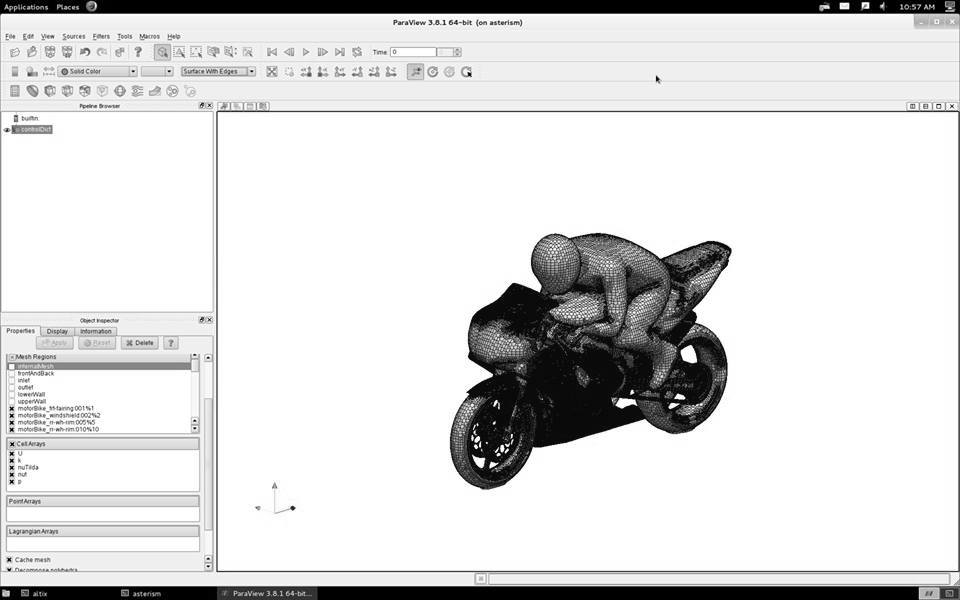
\includegraphics[scale=0.5]{image201604/motorbike_mesh_mono.jpg}

\subsection{解析結果を実行する}
解析を実行してみましょう。
今回のチュートリアルは、非圧縮性の粘性流体を PISO 法で解きます。
このアルゴリズムは、pisoFoam というアプリケーションで利用できます。
移流項の空間離散は 1 次風上差分、拡散項は 2 次精度の中心差分を利用しています。
これらは、\verb|system/fvSchemes| で設定されています。
線形ソルバは AMG 前処理ありの CG 法を使用します。
こちらは、\verb|system/fvSolutions| で設定されています。

\subsection{解析結果を見てみる}
解析は終了しましたが、解析結果はデータファイルとして出力されただけです。
数値ファイルから、数百万点の要素を持つメッシュから空気の流れを読み取ることなどは
ほぼ不可能です。
そのため、解析結果のデータファイルを人間が目で見て理解できるように表示してくれる
可視化ソフトを使用します。
すでにメッシュ作成のところで紹介済みですが、ここでも paraview を使用します。\\
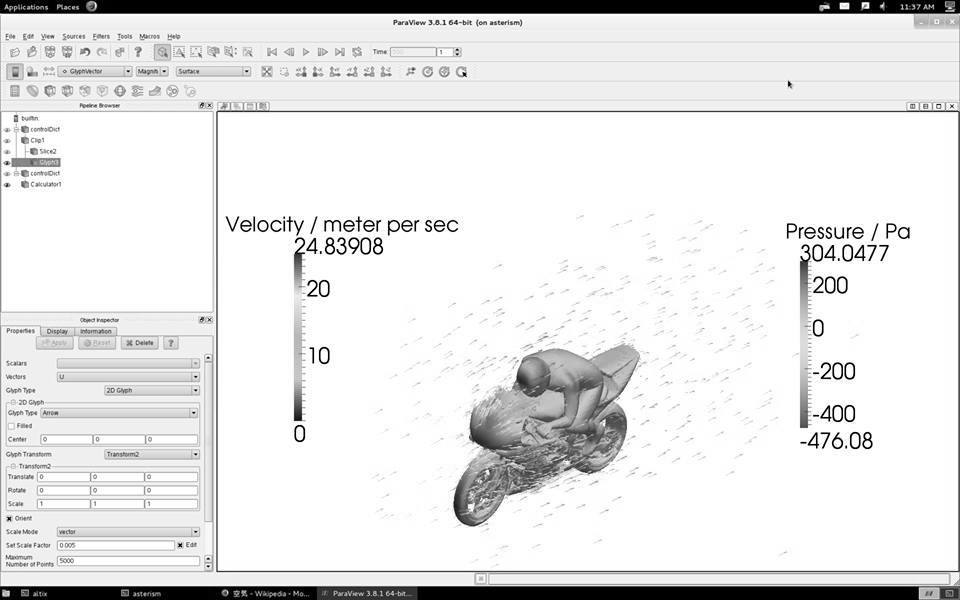
\includegraphics[scale=0.5]{image201604/motorbike_velocity_and_pressure_mono.jpg}

\subsection{まとめ}

\subsubsection{良い点}
OpenFOAMは、商用ソフトと比べて数学的な法則に乗っとてくれているので嬉しいです。商
用のソフトは、数値解析の安定性を確保するために、数学的なトリックを多用しているこ
とが多いです。
1000並列ぐらいまでならば、問題なくスケーリングすることが知られています。ただし、
理論性能比は察してください。
そして、ソースコードさえ読めれば、どんな機能でも自分でカスタマイズなどができるこ
とです。

\subsubsection{悪い点}
数値解析の安定性はあまり良くないです。かなりの数値流体の知識が要求されます。
Unix/Linux に詳しくない技術者にはとっつきにくいかもしれない。

%201606 Debian / Ubuntu ユーザーミートアップ in 札幌
\dancersection{Debianパッケージの “説明文” について} {吉野 与志仁}

\subsection{自己紹介}

吉野 与志仁(よしの よしひと,@yy\_y\_ja\_jp)です。
Debian 公式開発者ではないです。manpages-ja パッケージのメンテナです。Debian JP Project メンバーです。

\subsection{Agenda}
 Debianパッケージの “説明文” について。
\begin{enumerate}
   \item Debian とは?
%   \item Universal
   \item パッケージ
   \item DDTP / DDTSS
   \item まとめ
% XXX
\end{enumerate}

\subsection{Debian とは?}


 \url{https://www.debian.org/}


 \begin{center}
  
\includegraphics[width=\hsize]{image201606/banner_mono.png}
 \end{center}


 Debian -- The Universal Operating System
\begin{itemize}
 \item The  -- 一つしかない
 \item Universal  -- 普遍的な
 \item Operating System  -- オペレーティングシステム (OS)
\end{itemize}

\subsection{Operating System}
 Operating System -- オペレーティングシステム (OS)

 \begin{itemize}
  \item “コンピュータを動作させるために必要な基本プログラムとユーティリティ
	の集合体”
  \item “Debian は、純粋な OS 以上の機能を提供します。あなたのコンピュー
	タに手軽にインストールできるよう 43000 を越すコンパイル済ソフト
	ウェアが パッケージとして付属しています。”
 \end{itemize}

 ざっくり言うと
 \begin{itemize}
  \item コンピュータを動かすもの
  \item あなたの使いたいソフトを手軽にインストールできるもの
 \end{itemize}

\subsection{Universal Operating System}
\begin{itemize}
 \item Universal -- 普遍的な
 \item Operating System -- オペレーティングシステム (OS)
\end{itemize}
 Debian は
 \begin{itemize}
  \item 様々なコンピュータ(ハードウェア)を動かせます\\
	-- アーキテクチャ・移植版(amd64, arm64, ...)
  \item 様々なソフトウェアを手軽にインストールできます\\
	-- 43000 を越すパッケージ
 \end{itemize}

 Debian を
 様々な人々が使えます
 %  \item 誰に
 \begin{itemize}
  \item 人種・民族・言語 -- 翻訳\\
	Debian のインストーラ(d-i)は75 (22)言語に対応
%  \item 性別・ジェンダー -- Debian Women
  \item 年齢 -- Debian Jr., Debian Edu, ...
  \item 障碍\\
	d-i は点字ディスプレイに対応\\
	Debian Accessibility, ...
%  \item …
 \end{itemize}

\subsection{パッケージ}

\begin{itemize}
 \item ソフトウェアを手軽にインストールできるようにしたもの
 \item 各パッケージには基本的に必ず責任者(メンテナ)が存在\\
       -- Debian はコミュニティベースなので、基本ボランティア\\
       そのソフトウェアを多くの人に使ってもらいたいという思いがある人な
       ど(そのソフトウェアの業界の人や、そのソフトウェアの作者自身であることも)
 \item 各パッケージには“control”ファイルが含まれ、それに基づいて管理されている
\end{itemize}

\subsection{control ファイルの例(jessie の nginx パッケージ)}

{\scriptsize{%
\begin{verbatim}
Package: nginx
Version: 1.6.2-5+deb8u2
Architecture: all
Maintainer: Kartik Mistry <kartik@debian.org>
Installed-Size: 99
Depends: nginx-full (>= 1.6.2-5+deb8u2) | nginx-light (>= 1.6.2-5+deb8u2) | nginx-extras (>= 1.6.2-5+deb8u2), \\
nginx-full (<< 1.6.2-5+deb8u2.1~) | nginx-light (<< 1.6.2-5+deb8u2.1~) | nginx-extras (<< 1.6.2-5+deb8u2.1~)
Section: httpd
Priority: optional
Homepage: http://nginx.net
Description: small, powerful, scalable web/proxy server
 Nginx ("engine X") is a high-performance web and reverse proxy server
 created by Igor Sysoev. It can be used both as a standalone web server
 and as a proxy to reduce the load on back-end HTTP or mail servers.
 .
 This is a dependency package to install either nginx-full (by default) or
 nginx-light.
\end{verbatim}
}}

\subsection{パッケージ}
   たくさんあるパッケージからどうやって選びますか?

   パターン1
   \begin{enumerate}
    \item ぐぐる
    \item 誰かのブログ記事を読む「〜という名前のパッケージをインストール
	  しましょう」
    \item それに従うか決める
   \end{enumerate}

   パターン2
   \begin{enumerate}
    \item ぐぐる
    \item Debian のパッケージページに行き着く\\
	  -- 内容は control ファイルの中身とほぼ同じ
    \item 読んでインストールするか決める
   \end{enumerate}

   \begin{center}
  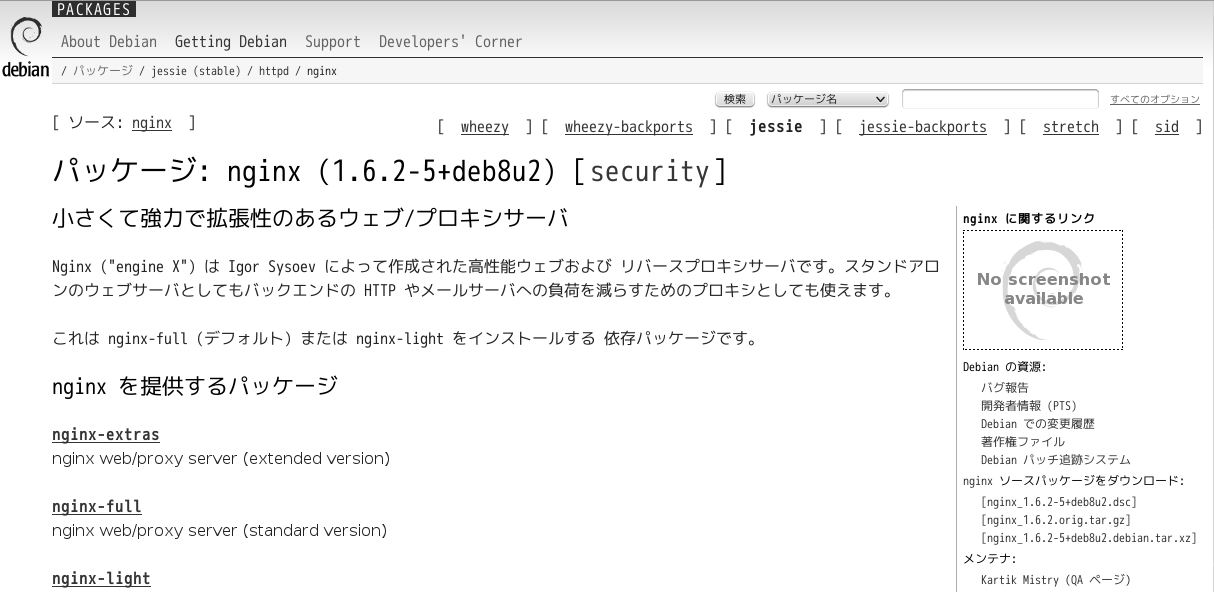
\includegraphics[width=0.9\hsize]{image201606/pdo_mono.png}
   \end{center}


\subsection{control ファイルの中身}
  Package -- パッケージの名前 (例: \verb+Package: nginx+)
\\
  Maintainer -- パッケージのメンテナ
  例: \verb+Maintainer: Kartik Mistry <kartik@debian.org>+
\\
  Section -- パッケージの分類 (例: \verb+Section: httpd+)

%  {\scriptsize{
%admin         (管理ユーティリティ),
%cli-mono      (Mono/CLI),
%comm	      (コミュニケーションプログラム),
%database      (データベース),
%debug	      (デバッグパッケージ),
%devel	      (開発),
%doc	      (ドキュメント),
%editors	      (エディタ),
%education     (教育),
%electronics   (電子工学),
%embedded      (組み込みソフトウェア),
%fonts	      (フォント),
%games	      (ゲーム),
%gnome	      (GNOME),
%gnu-r	      (GNU R),
%gnustep	      (GNUstep),
%graphics      (グラフィック),
%hamradio      (アマチュア無線),
%haskell	      (Haskell),
%httpd	      (ウェブサーバ),
%interpreters  (インタプリタ),
%introspection (Introspection),
%java	      (Java),
%kde	      (KDE),
%kernel	      (カーネル),
%libdevel      (ライブラリ開発),
%libs	      (ライブラリ),
%lisp	      (Lisp),
%localization  (言語パック),
%mail	      (メール),
%math	      (数学),
%metapackages  (メタパッケージ),
%misc	      (その他),
%net	      (ネットワーク),
%news	      (ニュースグループ),
%ocaml	      (OCaml),
%oldlibs	      (旧式ライブラリ),
%otherosfs     (異なるオペレーティングシステムやファイルシステムのもの),
%perl	      (Perl),
%php	      (PHP),
%python	      (Python),
%ruby	      (Ruby),
%science	      (科学),
%shells	      (シェル),
%sound	      (サウンド),
%tasks	      (タスク),
%tex	      (\TeX),
%text	      (テキスト処理),
%utils	      (ユーティリティ),
%vcs	      (バージョン管理システム),
%video	      (映像),
%web	      (ウェブソフトウェア),
%x11	      (X ウィンドウシステムのソフトウェア),
%xfce	      (Xfce),
%zope	      (Zope/Plone フレームワーク),
%}}
%\\
  Description -- パッケージの説明文

  \begin{itemize}

   \item Debian Policy 3.4
	 \begin{itemize}
	  \item 初めて見た人がインストールしたいか判断できるように書くべ
		しとされている
	  \item 重要なことは説明文の出だしに書くことになっている
	 \end{itemize}
   % \item control ファイルのDescriptionは英語
%	 英語の読めない人・苦手な人に翻訳が必要
%   \end{itemize}

% \begin{itemize}
 \item 1行目 -- short description (短い説明文)\\
       例:\\
       {
  \scriptsize
\begin{verbatim}
Description: small, powerful, scalable web/proxy server
\end{verbatim}
}
 \item 2行目以降 -- long description (長い説明文)\\
       例:\\
  \scriptsize
\begin{verbatim}
 Nginx ("engine X") is a high-performance web and reverse proxy server
 created by Igor Sysoev. It can be used both as a standalone web server
 and as a proxy to reduce the load on back-end HTTP or mail servers.
 .
 This is a dependency package to install either nginx-full (by default) or
 nginx-light.
\end{verbatim}
  \end{itemize}

\subsection{Description -- パッケージの説明文}
   control ファイルのDescriptionは英語

   Debian はコミュニティベースなので、誰かボランティアが翻訳する


   \begin{itemize}
    \item パッケージになっているソフトウェアを知らないと正しく翻訳できない
    \item Universal なのでソフトウェアの分野(業界)が幅広く、少人数でやるのは困難
   \end{itemize}
   ⇒ 自分の普段使っているパッケージ・自分の専門分野のパッケージなら翻訳できるはず!

\subsection{DDTP -- Debian Description Translation Project / DDTSS }

 \url{http://ddtp.debian.net/}

  \begin{itemize}
   \item パッケージのDescriptionを翻訳するプロジェクト
   \item Debian 公式開発者でなくても作業できます
   \item 日本語チームの方針: 翻訳の品質を向上させること。量ではない
     {\scriptsize (でも原文の伸びはすごい…)}
  \end{itemize}

  \begin{center}
  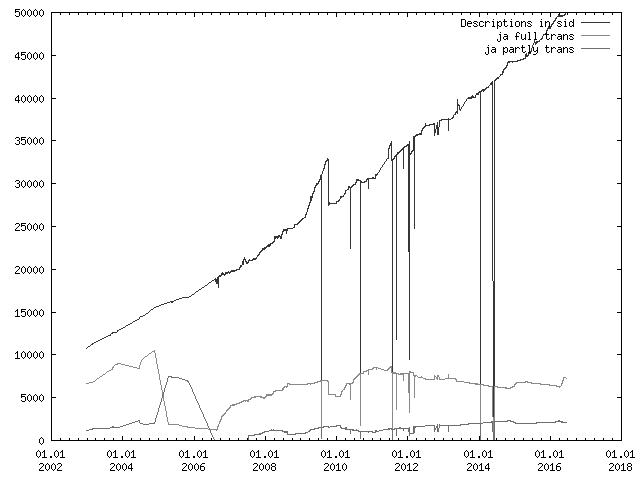
\includegraphics[width=0.65\hsize]{image201606/stat-trans-sid-ja_mono.png}
  \end{center}

\subsection{DDTP -- Debian Description Translation Project}
   言語別統計

   \begin{center}
  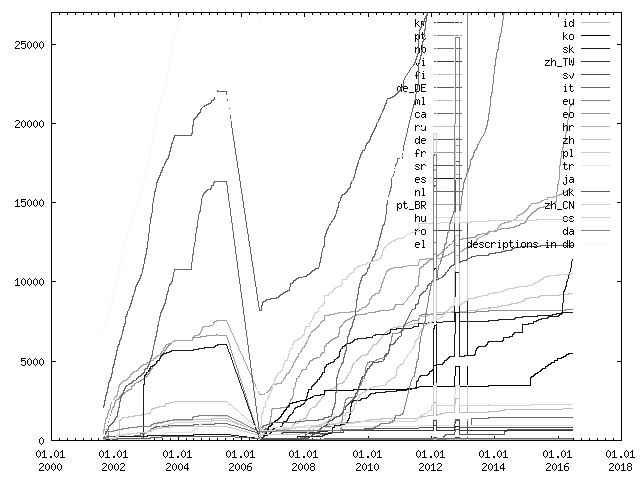
\includegraphics[width=0.65\hsize]{image201606/ddts-stat_mono.png}
   \end{center}

\subsection{DDTP -- Debian Description Translation Project}
   言語別・Priority別統計

   \begin{center}
  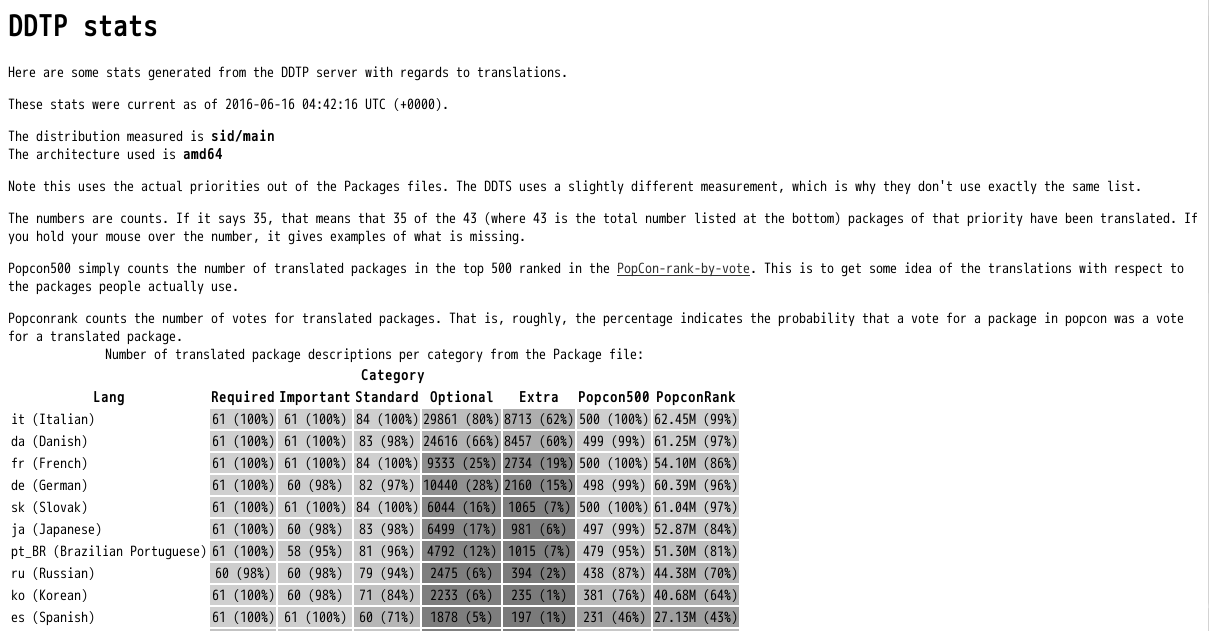
\includegraphics[width=\hsize]{image201606/stats-sid_mono.png}
   \end{center}

\subsection{DDTSS}
   Web でDescriptionの翻訳・レビュー・修正ができるサイト\\
   日本語への翻訳は
   \url{http://ddtp.debian.net/ddtss/index.cgi/ja}

   \begin{center}
  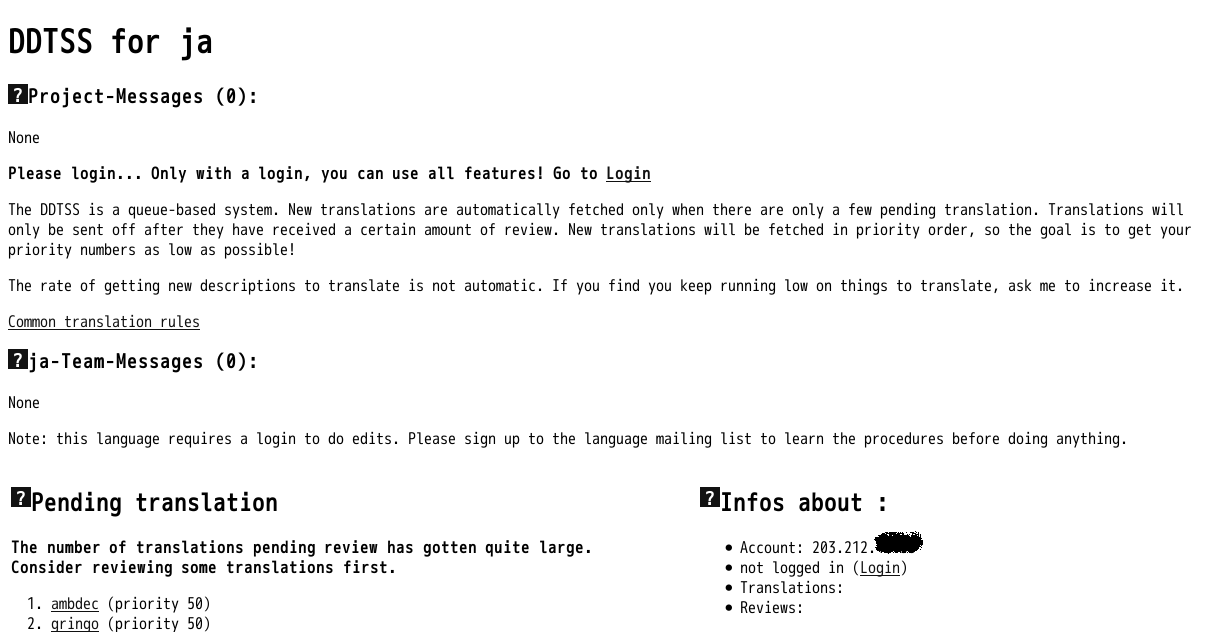
\includegraphics[width=0.9\hsize]{image201606/ddtss-anonymous_mono.png}
   \end{center}

\subsection{DDTSS}
    Debian 公式開発者でなくても作業できます\\
    誰でもアカウントを作成して翻訳・レビュー・修正ができます

   詳しくは 第53回東京エリアDebian勉強会(2009年6月勉強会)の資料など\\
   \url{https://tokyodebian.alioth.debian.org/2009-06.html}

   \begin{center}
  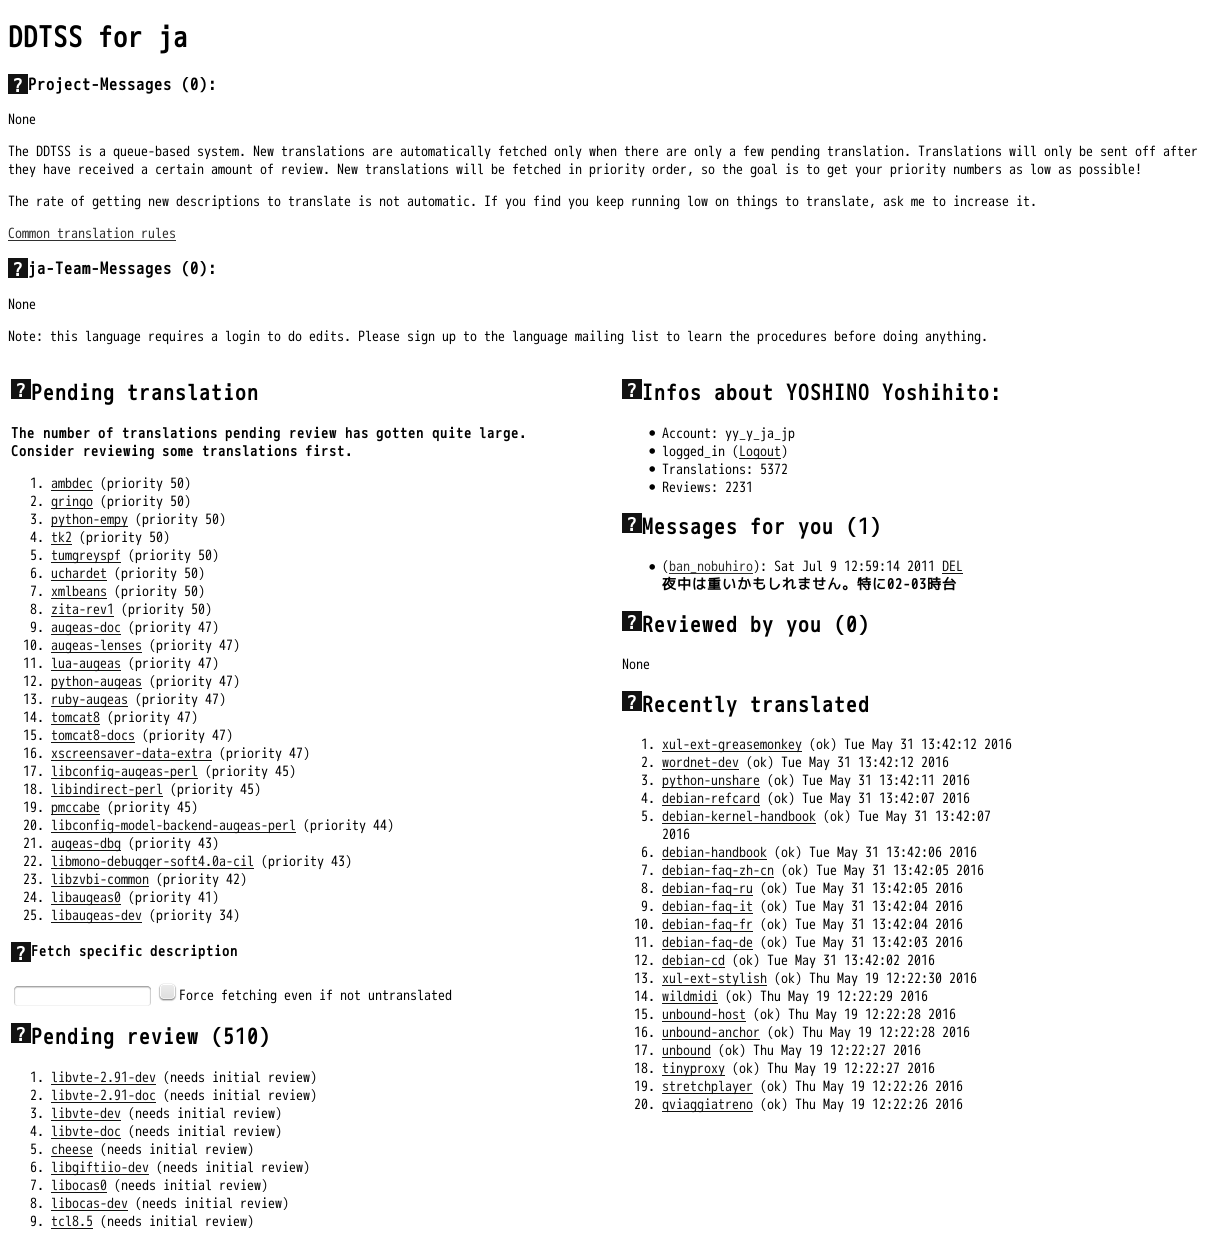
\includegraphics[width=0.9\hsize]{image201606/ddtss_mono.png}
   \end{center}

  3人がレビューすると翻訳済みになり、その説明文が Debianのレポジトリに反映されます

  \begin{center}
  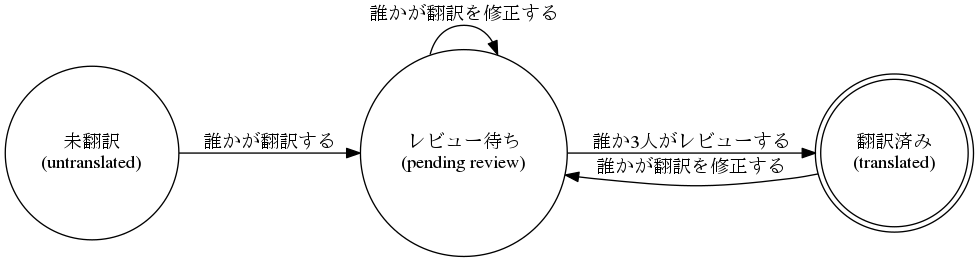
\includegraphics[width=0.9\hsize]{image201606/ddtss-flow_mono.png}
   \end{center}

\subsection{まとめ}

 \begin{itemize}
  \item Debian は Universal な OS なので
	\begin{itemize}
	 \item 幅広い分野のソフトウェアのパッケージが多数ある\\
	   -- その中からインストールしたいものを選ぶきっかけとして、パッケージ名、説明文などがある
	 \item 様々な母国語・言語のユーザーが使う ⇒ 翻訳を提供
	\end{itemize}
      \item Debian はコミュニティベースなので基本ボランティア\\
        -- パッケージのメンテナンス、翻訳、…
  \item 日本語チームとしては、質の高い日本語でパッケージ説明文を日本語ユー
	ザーに提供したい
  \item DDTSS で誰でも説明文の翻訳ができます
  \item パッケージのソフトウェアやその分野(業界)を知らないと翻訳ができない。質の高い翻訳もできない\\
    ⇒ ユーザーのみなさん、お使いのパッケージの翻訳・レビュー・修正にご協力ください!\\
    みなさん、あなたの専門分野のパッケージの翻訳・レビュー・修正にご協力ください!
 \end{itemize}

\subsection{補足1}

質問:DDTSS にアクセスしてみたいのですが、つながりません。\\

  ⇒ はい、5月からつながりません。今のところ /etc/hosts に次の行を追加してください。

  117.121.245.169 ddtp.debian.net
\\
2016年8月末から、 https://ddtp2.debian.net でアクセス出来るようになりました。\footnote{https://lists.debian.org/debian-i18n/2016/08/msg00011.html}

\subsection{補足2}


  \begin{itemize}
  \item 小学生でも英語が必修なのに、翻訳する意味はあるのですか?\\

    ⇒ パッケージのメンテナは英語が苦手な人にも使ってもらいたいと思っているでしょう。

   \item 私の専門分野のパッケージはありますが、日本語はオワコンです。翻
	 訳する意味はあるのですか?\\

	 ⇒ 英語が苦手な人でもパッケージを使ってくれるようになれば、その人があな
	 たの専門分野に興味を持ってくれる可能性が高まると思います。

   \item 私の専門分野にある最近の用語には日本語訳がありません。\\

	 ⇒ その用語の部分はカタカナが業界的に通用しているならカタカナで、そうでないなら無理に訳さず英語のままでいいと思います。
  \end{itemize}

\dancersection{go-apt-cacher/mirror}{湯谷啓明}

サイボウズ株式会社 湯谷啓明です。
作成、公開したgo-apt-cacher/go-apt-mirrorについて説明します。

\subsection{go-apt-cacher/go-apt-mirrorとは}

\begin{itemize}
 \item Aptレポジトリに特化したキャッシュプロキシ/ミラーリングツール
 \item ハッシュの一致をチェックするので壊れない!
 \item Go製
\end{itemize}

GitHubで公開してます。
https://github.com/cybozu-go/aptutil

\subsection{CybozuとDebian}
\begin{itemize}
 \item サーバはUbuntu
 \item サービスに必要なコンポーネントはdebパッケージ化してAptレポジトリ(JFrog Artifactory)で集中管理
\end{itemize}
参考:社内利用のための deb パッケージング入門http://blog.cybozu.io/entry/2016/05/16/111500

\subsection{JFrog Artifactory}
\begin{itemize}
 \item アーティファクト管理ツール
 \item OSS 版は Maven レポジトリ機能のみ
 \item 商用版は apt, yum, npm, PyPI, … と多種
 \item REST API で CI/CD ツールと連携できる
 \item リモートレポジトリのミラーはできない
 \item リバースプロキシ兼キャッシュはできる
\end{itemize}

\subsection{キャッシュ/ミラーが必要な理由}
\begin{itemize}
 \item Artifactoryの負荷を減らしたい
 \item パッケージダウンロードを速くしたい
\end{itemize}

\begin{itemize}
 \item 更新頻度が高く、ファイルが少ない\mbox{}\\
 → 必要なものだけキャッシュ
 \item 更新頻度が低く、ファイルが多い\mbox{}\\
 → (レポジトリの一部を)まるごとミラー
\end{itemize}

\subsection{go-apt-cacherの特徴}
\begin{itemize}
 \item ReleaseやPackagesからチェックサム情報を抽出
\begin{itemize}
 \item ダウンロードしたファイルのチェックサムが合わなければ破棄
 \item Release は定期的にチェックし、チェックサムが更新されたファイルのキャッシュは自動破棄
\end{itemize}
 \item HTTP ヘッダは無視
\begin{itemize}
 \item キャッシュした Release を定期的に自動更新
 \item 他のファイルは上記チェックサム変更の自動破棄で対応
\end{itemize}
 \item Go なので速い
\begin{itemize}
 \item 同時 1,000 クライアントも余裕
 \item キャッシュ済みファイルは 1ms 以下で処理
\end{itemize}
\end{itemize}
\subsection{go-apt-mirrorの特徴}
\begin{itemize}
 \item 部分的ミラー
\begin{itemize}
 \item Suite, Section, Architecture, Source を指定
 \item 必要なものだけミラー
\end{itemize}
 \item rsync より高速な更新
\begin{itemize}
 \item インデックスを先に処理してファイルのチェックサム情報を入手
 \item 以前と変化がなければローカルファイルシステム上で再利用
\end{itemize}
 \item 不完全なミラーは決して作らない
\begin{itemize}
 \item インデックスおよびファイルのチェックサムはすべてチェック
 \item 正しいセットが作れない場合、ロールバック
\end{itemize}
 \item ミラーの更新がアトミック
\begin{itemize}
 \item 更新中の状態は決して見せない
\end{itemize}
\end{itemize}
\subsection{実装で大変だったところ}
Debian Control Fileのパース
\begin{itemize}
 \item 存在しないファイルがRelease/Packagesに記載されている
 \item ファイルはひとつのインデックスだけに書かれているとは限らない
 \item ファイルが存在しないと違うフォーマットのファイルを返してくる
 \item …
\end{itemize}
\subsection{Feedbacks are welcome!!}
リリースしたばかりなのでバグもあると思いますが、よければ使ってみてください\\
※弊社での必要性に応じて作られたツールで、既存のツールを置き換えるものではありません

%201610kansai
\dancersection{sbuild と debci を触ってみた}{佐々木洋平}

\subsection{はじめに}
  Debian パッケージを作成する際に「ビルド時の依存関係を満たしているのか」だけではなく
  「そのパッケージの更新による他のパッケージへの影響/不具合はどうなのか」という懸念があります。
  %
  今回の発表では、pkg-ruby-extra team で導入している
  \texttt{sbuild} + \texttt{debci} という環境を例に、
  それらの懸念をどの様に解消しているのかについて簡単にまとめてみました

%というわけで、先ずは \texttt{sbuild} と \texttt{debci} について簡単にまとめてみます。

\subsection*{sbuild とは?}

\url{https://wiki.debian.org/sbuild} より抜粋:
\begin{quote}
  \texttt{sbuild} is used on the official buildd network to build binary
  packages for all supported architectures.
  %
  It can also be used by individuals to test that their package builds
  in a minimal installation of Debian Unstable.
  %
  In particular, this helps ensure that you haven't missed any build
  dependencies.
  \\[1em]
  The main alternative to sbuild is \texttt{pbuilder} combined with \texttt{cowbuilder}.
\end{quote}
というわけで、\texttt{sbuild} は
「\textbf{公式の buildd network で使用されている}」クリーンルームビルド環境です。
同様のパッケージ作成環境には(上記 Wiki で触れられている通り)
\texttt{pbulider} や \texttt{cowbuilder} があります
\footnote{%
  \texttt{pbulider} や \texttt{cowbuilder} に
  対して、\texttt{sbuild} は何が嬉しいのでしょうか?
  調べてみましたが、どちらかに絶対的な優位性がある、といった話でも無さそうです。
  慣れている方を使ったら良いのではないか、という無難な結論になりそうですね。
  強いて言えば、既に触れた通り
  「公式配布パッケージ群のビルド環境である」という点が優位な所でしょうか?
}。

\subsection*{debci とは?}

\texttt{debci} は Debian パッケージに関する
CI -- Continuous Integration
つまり「ビルドやテストを継続的に実行することで品質改善を行なう」ためのフレームワークです。
%
Debian パッケージの「テスト」に関する枠組みとしては既に
\begin{itemize}
\item %
  \texttt{piuparts} による「パッケージとしての品質」のテスト
\item %
  \texttt{autopkgtest} による「ソフトウェアとしての」テスト
\end{itemize}
があります。これらに加えて
\texttt{debci} では
\begin{center}
  パッケージを更新した際に、依存する他のパッケージが正しく動作するか
\end{center}
を「テスト」しています
(パッケージが正しく動作するか、は\texttt{autopkgtest} を用いています)。
%
実際に debci が動作している状況は
\url{https://ci.debian.net/} で見ることができます。
\begin{figure}[ht!]
  \centering
  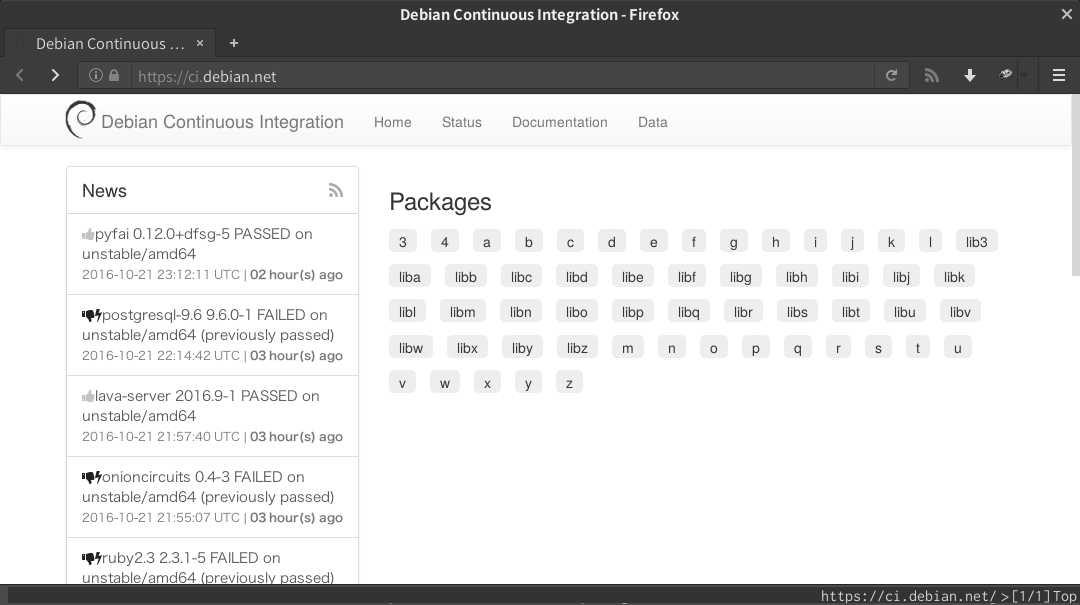
\includegraphics[height=.2\textheight]{image201610/screenshot-debci_mono.png}
  \caption{debci の screenshot: \url{https://ci.debian.net/}}
\end{figure}

\subsection{sbuild, debci の setup}

pkg-ruby-extras team の \texttt{setup} スクリプトは以下の通りです:
\begin{commandline}
#!/bin/sh

set -exu

sudo apt-get install -qy \
  autopkgtest \
  build-essential \
  gem2deb \
  git \
  git-buildpackage \
  myrepos \
  quilt \
  sbuild \
  lxc \
  debci \
  ""

sudo mkdir -p /root/.gnupg # To work around #792100
sudo sbuild-update --keygen
sudo sbuild-adduser $USER

chrootname=unstable-$(dpkg --print-architecture)-sbuild
chroot=/srv/chroots/$chrootname
if schroot --list --all-source-chroots  | grep unstable-amd64-sbuild; then
  :
else
  sudo sbuild-createchroot unstable $chroot http://httpredir.debian.org/debian
fi
for conf in $(grep -l '^union-type=' /etc/schroot/chroot.d/*-sbuild*); do
  if ! grep -q "^union-overlay-directory=" "$conf" ; then
    echo 'union-overlay-directory=/dev/shm' | sudo tee --append "$conf"
  fi
done

if ! grep -q /var/cache/apt/archives /etc/schroot/sbuild/fstab; then
  sudo sh -c 'echo /var/cache/apt/archives /var/cache/apt/archives none rw,bind 0 0 >>/etc/schroot/sbuild/fstab'
fi

# configure lxc networking if needed
if grep -q '^lxc.network.type\s*=\s*empty' /etc/lxc/default.conf; then
  sudo apt-get install -qy libvirt-clients libvirt-daemon-system iptables ebtables dnsmasq-base
  if ! (sudo virsh net-list | grep -q default); then
    sudo virsh net-start default
    sudo virsh net-autostart default
  fi
  sudo sed -i -e '/lxc.network.type/d' /etc/lxc/default.conf
  sudo tee --append /etc/lxc/default.conf <<EOF
lxc.network.type = veth
lxc.network.link = virbr0
lxc.network.flags = up
EOF
  sudo tee /etc/sudoers.d/lxc <<EOF
%sudo       ALL = NOPASSWD:SETENV: /usr/bin/lxc-*, /usr/bin/timeout
EOF

fi

sudo debci setup
\end{commandline}
% $

\subsection{sbuild: 1st step}

前半部分を参考に、先ずは \texttt{sbuild} を設定してみます。
何も考えなければ、
\begin{commandline}
sudo mkdir -p /root/.gnupg # To work around #792100
sudo sbuild-update --keygen
sudo sbuild-adduser $USER
chrootname=unstable-$(dpkg --print-architecture)-sbuild
chroot=/srv/chroots/$chrootname
sudo sbuild-createchroot unstable $chroot http://ftp.jp.debian.org/debian
for conf in $(grep -l '^union-type=' /etc/schroot/chroot.d/*-sbuild*); do
  if ! grep -q "^union-overlay-directory=" "$conf" ; then
    echo 'union-overlay-directory=/dev/shm' | sudo tee --append "$conf"
  fi
done
if ! grep -q /var/cache/apt/archives /etc/schroot/sbuild/fstab; then
  sudo sh -c 'echo /var/cache/apt/archives /var/cache/apt/archives none rw,bind 0 0 >>/etc/schroot/sbuild/fstab'
fi
\end{commandline}
% $
でしょうか?
\footnote{%
  GPG の鍵生成に時間がかかる場合には \texttt{havedged} 等で entropy を増やすと良いでしょう
}
上記によって、
\begin{itemize}
\item %
  union-fs による差分管理
\item %
  \texttt{/var/cache/apt/archives} を親と共有(bind mount)
\end{itemize}
した unstable-\texttt{\$arch} の sbuild 環境ができあがります。
\texttt{eatmydata} や \texttt{ccache} を加えておきたい場合には、
\begin{commandline}
  sudo sbuild-createchroot \
    --include=eatmydata,ccache,gnupg \
    unstable /srv/chroot/unstable-amd64 http://ftp.jp.debian.org/debian
\end{commandline}
の様に \texttt{--include} で含めておくパッケージを指定しておきます。

sbuildの簡単な使い方を簡単にまとめると以下の通りです。
\begin{itemize}
\item %
  環境設定: \texttt{~/.sbuildrc} に以下を書いておきます\footnote{%
    build 後に autopkgtest を走らせる設定もあるんですが、これは後程。
}
  \begin{commandline}
# -*- mode: cperl-mode
## basic
# architecture: all も build する
$build_arch_all = 1;
# デフォルトで source packag も build する
$build_source = 1;
## debsign
# GPG key id
$key_id = 'Your GPG Key ID';
# distribution の指定
$distribution = 'unstable';
## lintinan
# build 後に lintian を走らせる
$run_lintian = 1;
# lintian の option. お好みで。
$lintian_opts = ['-i', '-I'];
## piuparts
# build 後に piuparts を走らせる
$run_piuparts = 1;
# piuparts の option。ここでは schroot で走らせる
$piuparts_opts = ['--schroot', 'unstable-amd64-sbuild'];
  \end{commandline}
%$
\item %
  環境更新
  \begin{commandline}
    % sudo sbuild-update -udcar unstable-$arch
  \end{commandline}
  % $
  \texttt{-udcar} を指定することで
  "apt-get update; dist-upgrade; clean; autoclean; autoremove" が実行されます。
\item %
  パッケージのビルド:
  \texttt{dsc} がある場合
  \begin{commandline}
    % sbuild *.dsc
  \end{commandline}
  パッケージのビルド:パッケージのソースディレクトリで
  \begin{commandline}
    % sbuild
  \end{commandline}
\item %
  偶に schroot の session が残るので、綺麗にしましょう:
  \begin{commandline}
    % sudo schroot --end-session --all-sessions
  \end{commandline}
\end{itemize}
ざっくりとまとめると、こんな感じです。
\texttt{pbuilder} の様に「tar.gz の展開/chroot」という段階が無いため、
体感時間は短いです。また、結果の出力が fancy ですね。

\subsection{debci: 1st step}

次に \texttt{debci} を設定してみます。
スクリプトの該当部分は以下:
\begin{commandline}
# configure lxc networking if needed
if grep -q '^lxc.network.type\s*=\s*empty' /etc/lxc/default.conf; then
  sudo apt-get install -qy libvirt-clients libvirt-daemon-system iptables ebtables dnsmasq-base
  if ! (sudo virsh net-list | grep -q default); then
    sudo virsh net-start default
    sudo virsh net-autostart default
  fi
  sudo sed -i -e '/lxc.network.type/d' /etc/lxc/default.conf
  sudo tee --append /etc/lxc/default.conf <<EOF
lxc.network.type = veth
lxc.network.link = virbr0
lxc.network.flags = up
EOF
  sudo tee /etc/sudoers.d/lxc <<EOF
%sudo       ALL = NOPASSWD:SETENV: /usr/bin/lxc-*, /usr/bin/timeout
EOF

fi

sudo debci setup
\end{commandline}
これは
\begin{itemize}
\item %
  lxc の network は dnsmasq で良きにはからう
\item %
  debci の lxc backend の設定を行なう
\end{itemize}
といった塩梅です。このうち lxc 自体の設定は
\texttt{debci setup} の実態は
\texttt{/usr/share/debci/backends/lxc/create-testbed} です。
この中で lxc の設定が行なわれています。

...といった所で、資料執筆の時間が過ぎてしまいました。
実際に \texttt{debci} を触ってアレコレするのは当日の実演\&次の機会にまとめたいと思います。

%201606 tokyo
%-------------------------------------------------------------------------------
\dancersection{debexpo(mentors.d.n)をハックするには}{林健太郎(kenhys)}
%-------------------------------------------------------------------------------

\subsection{はじめに}

そのへんに生えているDebian使いがDebian公式パッケージを更新するにあたっては、更新したパッケージをDebian開発者にスポンサーしてもらう必要があります。

その際のパッケージのアップロード先には、mentors.debian.netというWebサイトがよく使われています。

今回はmentors.debian.netをハックする機会があったので、その内容を紹介します。\footnote{2016年8月現在の情報で、現在では若干記述が古くなっている箇所があります。該当箇所には注記を入れてあります。}

\subsection{debexpoとは?}

http://mentors.debian.net(以下mentors.d.n)を支えるウェブアプリケーションのことです。リポジトリ名がdebexpoになっています。

\begin{center}
\includegraphics[width=0.5\hsize]{image201606/mentors.d.n.eps}
\end{center}

debexpoの公式サイトは\url{https://alioth.debian.org/projects/debexpo/}です。
以前開発の中心となっていたサイト\url{https://workaround.org/project/debexpo}にはdebexpoの名前の由来が次のように記載されています。

\begin{quotation}
The new project was called "debexpo" because it was supposed to become an {\color{red}expo}sition for {\color{red}Deb}ian packages.
\end{quotation}

パッケージが一同に会する展覧会とでもいったところでしょうか。

\subsubsection{debexpo概要}

debexpoの位置付けがどういうものかなんとなくわかったところで、もうすこし具体的な紹介をしましょう。

debexpoの特徴をいくつか紹介すると以下があげられます。

\begin{itemize}
\item Python製
\item Pylons\footnote{\url{http://www.pylonsproject.org/}}フレームワーク採用
\item テンプレートエンジンはMako\footnote{\url{}}
\end{itemize}

このPylonsというフレームワーク、あまり知らない人がいるかも知れませんので補足しておくと、

\begin{itemize}
\item Railsっぽいフレームワーク
\item 2011年にメンテナンスモード入りした枯れたフレームワークです
\item 後継としてPyramidというフレームワークが開発されています
\end{itemize}

という特徴があります。

\begin{itembox}[l]{コラム:debexpoにもゆるキャラが?}
\includegraphics[width=0.2\hsize]{image201606/debexpo-mascot-zoom.eps}
debexpoには、実はゆるキャラが設定されています。Webサイトの左上隅の赤枠で囲っているところに何かいますよね、それです。
ただし、詳細は不明です。SUUMO\footnote{不動産情報サイト。\url{http://suumo.jp/}}のスーモ\footnote{マスコットキャラクター。スーモの部屋\url{http://suumo.jp/edit/suumo-heya/}という特設ページがある。}には片思いのスモミとの想像上の子供スモルがいるという設定\footnote{\url{http://suumo.jp/edit/suumo-heya/character/suumo_character.pdf}}
があるくらいなので、このキャラにも何かありそうな気もしますが。。。
\end{itembox}

\subsection{なぜdebexpoをハックする必要が?}

パッケージをスポンサーしてもらうときに使うmentors.d.nにはいくつかお薦めな点があります。

\begin{itemize}
  \item パッケージのチェックもしてくれる
  \item RFSのテンプレートも生成してくれる
\end{itemize}

\begin{screen}
  \includegraphics[width=0.8\hsize]{image201606/qa-information.eps}
\end{screen}

スクリーンショットからもわかるように、QA informationの欄にLintianの警告などが表示されるようになっています。

\begin{screen}
  \includegraphics[width=0.5\hsize]{image201606/view-rfs-template.eps}
\end{screen}

また、スクリーンショットの「View RFS template」のリンクをたどると、RFSのテンプレートも生成してくれるというのも嬉しいポイントです。

なので、あとはこのRFSテンプレートをもとにして、メールするだけになっています。\footnote{とはいうものの、嘘ではないが、正確でもない。}

実際のRFS templateを見てみましょう。

\begin{screen}
\includegraphics[width=0.5\hsize]{image201606/rfs-template-pithole.eps}
\end{screen}

[fill in]の文字がちらほらあるのがわかりますね。

\begin{screen}
\includegraphics[width=0.5\hsize]{image201606/rfs-template-pithole2.eps}
\end{screen}

これだけではありません。ほかにも穴埋めが必要です。

\begin{screen}
\includegraphics[width=0.5\hsize]{image201606/rfs-template-fill-in1.eps}
\end{screen}

Subject:に種別を書かないといけません。

\begin{screen}
\includegraphics[width=0.5\hsize]{image201606/rfs-template-fill-in2.eps}
\end{screen}

Severity:を書かないといけません。

\begin{screen}
\includegraphics[width=0.5\hsize]{image201606/rfs-template-fill-in3.eps}
\end{screen}

Upstream,URL,License:を書かないといけません。

\begin{screen}
\includegraphics[width=0.5\hsize]{image201606/rfs-template-fill-in4.eps}
\end{screen}

Changelogを書かないといけません。

これで終わりでしょうか。いいえ違います。

\begin{screen}
\includegraphics[width=0.5\hsize]{image201606/rfs-template-fill-in5.eps}
\end{screen}

さりげなく埋めこまれたhelloとexample.comが残っています。

ようやくあれこれ直し終えました。これでメールが出せると、思うかも知れません。事実私も最初はそう思いました。

ここで問題になるのが、先頭に埋めこまれたスペース2つです。

\begin{screen}
\includegraphics[width=0.5\hsize]{image201606/rfs-template-pithole3.eps}
\end{screen}

ここで、上記はコマンドメールであることを思いださねばなりません。つまり、そのままメールするともちろんエラーになります。

したがって、「なぜdebexpoをハックするのか?」に対する答えは、「RFSテンプレートの残念っぷりをどうにかしたい」から、ということになります。

\begin{screen}
\includegraphics[width=1.0\hsize]{image201606/alioth-debexpo-313593-request.eps}
\end{screen}

Aliothをみてみると、同じ思いの人がいました。それはAliothのtrackerで4年も前に通った道だ、という。

\subsection{どうやってハックしたのか?}

おおむね、以下の流れでdebexpoをハックすることになりました。

\begin{itemize}
  \item upstream探し
  \item ドキュメント探し
  \item まずは動かしてみる
  \item あたりをつけて修正
  \item そしてPRへ
\end{itemize}

特別なことは何もなくて、よくあるフリーソフトウェアの修正です。

\begin{itembox}[l]{コラム:debexpoの歴史について}
debexpoは2003年に最初のコードがPerlで書かれました。しかし、機能拡張の要望に応えたりしていくには支障があったため、Pythonで書き直されたという経緯があります。
debexpoの開発が活発になったのは、2008年のことです。Google SoCに採択されたため、Jonny Lamb氏らにより一気に開発がすすみました。

2009年から2010年はゆるやかな開発が続きました。http://expo.debian.net/が公開されたのもこのころです。現在のmentors.d.nへと切り替えられたのは2011年のことです。
その後も、2012年にはUIの改善(debexpo v2)や再度GSoCへの採択(debexpo v3)などと開発が続いています。

このあたりの変遷について、Nicolas Dandrimont氏による「The State of mentors.debian.net GSOC and Beyond」という発表資料に詳しく書かれているので興味がある人は参照するとよいでしょう。
\footnote{\url{http://fr2012.mini.debconf.org/slides/debexpo.pdf}}
\end{itembox}

\subsubsection{upstream探し}

\begin{screen}
\includegraphics[width=0.5\hsize]{image201606/source-code-and-bugs.eps}
\end{screen}

debexpoの場合には、mentors.d.n下部にリンクがきちんとあるので、Aliothをみればいいとわかりました。

\begin{screen}
\includegraphics[width=0.5\hsize]{image201606/last-change-on-alioth.eps}
\end{screen}

ただ、どうやら最近はコミットがないのが不安になりました。
よく使われているならそこそこメンテされているイメージがあったからです。実際にはそうでもありませんでした。

\begin{screen}
\includegraphics[width=0.7\hsize]{image201606/last-change-on-github.eps}
\end{screen}

あとから、GitHubのほうが実は新しい\footnote{\url{https://github.com/debexpo/debexpo}}ことがわかりました。

実際の運用としては、Aliothがmaster\url{https://alioth.debian.org/projects/debexpo/}で、GitHubのをマージという運用になっているようです。

\subsubsection{ドキュメント探し}

リポジトリのdocs/*にドキュメントが整備されていました。インストール手順はdocs/installing.rstを参照すればよいとわかりました。
ただ、残念なことにその内容の一部はリンク先が404になってしまっていました。

\subsubsection{まずは動かしてみる}

ドキュメントから、セットアップ方法は3種類あることがわかりました。

\begin{itemize}
  \item 既存システムにインストール
  \item virtualenvでインストール
  \item VirtualBoxでインストール
\end{itemize}

まずはVirtualBoxで試してみることにしました。環境を分けたいのがその選択理由です。
ただ、Vagrantfileがアレな状態であることがわかりました。

\begin{screen}
\begin{minted}{sh}
# Every Vagrant virtual environment requires a box to build off of.
config.vm.box = "chef/debian-7.6"
\end{minted}
\end{screen}

Debian 7.6 (2014年7月12日)?になっていました。Debian 7.10がもうすでにでているご時世にも関わらずです。

vagrant upしてみるとまた残念な状態でした。

\begin{commandline}
$ vagrant up
Bringing machine 'default' up with 'virtualbox' provider...
==> default: Box 'chef/debian-7.6' could not be found. Attempting to find and install...
  default: Box Provider: virtualbox
  default: Box Version: >= 0
The box 'chef/debian-7.6' could not be found or
could not be accessed in the remote catalog. If this is a private
box on HashiCorp's Atlas, please verify you're logged in via
`vagrant login`. Also, please double-check the name. The expanded
URL and error message are shown below:

URL: ["https://atlas.hashicorp.com/chef/debian-7.6"]
Error: The requested URL returned error: 404 Not Found
}
\end{commandline}

boxが見つからなくてコケていました。そこで、PR\#32で修正しました。
失敗していたのは、Bento projectに移行していたせいでした。

\begin{screen}
\includegraphics[width=0.7\hsize]{image201606/debexpo-pr32-use-latest-wheezy.eps}
\end{screen}

起動して、ログインするには次のようにします。

\begin{commandline}
$ vagrant up --provision
$ vagrant ssh
\end{commandline}

vagrant sshしてpasterコマンドを実行してサーバーを起動します。

\begin{commandline}
$ cd debexpo
$ . venv/bin/activate
$ paster serve development.ini
\end{commandline}

このようにすると、5000ポートでサーバーを起動することができます。

\begin{screen}
\includegraphics[width=0.5\hsize]{image201606/debexpo-on-localhost.eps}
\end{screen}

これによりブラウザでアクセス可能になります。

次にユーザーの追加をします。方法は2つあって、ブラウザ経由で追加するのと、JSONをもとに追加するやりかたがあります。

\begin{screen}
\includegraphics[width=0.5\hsize]{image201606/debexpo-sign-me-up.eps}
\end{screen}

JSONで追加するなら次のような内容のファイルを用意します。

\begin{screen}
\begin{minted}{javascript}
{
  "realname":"Hayashi Kentaro",
  "password":"password",
  "email":"hayashi@clear-code.com"
}
\end{minted}
\end{screen}

ユーザー追加用のスクリプトが用意されているので、それを利用します。

\begin{commandline}
$ python ./bin/user_importer.py -i development.ini -u user.json
\end{commandline}

次にアカウントの有効化をします。アカウントを有効にするには2つ設定をする必要があります。

\begin{itemize}
\item verification (ログインに必要)
\item dmup (アップロードに必要)
\end{itemize}

verificationの設定は次のようなクエリを実行することで行います。

\begin{screen}

\includegraphics[width=0.7\hsize]{image201606/update-verification.eps}
\end{screen}

verificationを空にすることで、メールによる確認プロセスを迂回することができます。

もう一つ、DMUPとはマシン使用ポリシーのことです。開発で使うだけなので、次のようなクエリを実行することでdmupフィールドを更新して、同意したことにします。

\begin{screen}

\includegraphics[width=0.7\hsize]{image201606/update-dmup.eps}
\end{screen}


ここまでできたら、あとはアップロードするために、.dput.cfの設定をします。

\begin{screen}
\begin{minted}{sh}
[debexpo]
fqdn = localhost:5000
incoming = /upload/kenhys@gmail.com/password
method = http
allow_unsigned_uploads = 0
\end{minted}
\end{screen}

用意できたら、実際にアップロードを試してみましょう。

\begin{commandline}
Uploading to debexpo (via http to localhost:5000):
Uploading groonga_6.0.2-1.dsc:
Upload failed: 500 Internal Server Error
\end{commandline}

と思ったら、あっさり500 Internal Server Errorに遭遇しました。

\begin{screen}
\includegraphics[width=0.7\hsize]{image201606/find-a-debexpo-bug.eps}
\end{screen}

残念なことに、あるべきディレクトリがないというオチでした。

そこで、PR\#34で修正してとりこんでもらいました。

\begin{screen}
\includegraphics[width=0.7\hsize]{image201606/debexpo-pr34-incoming-directory.eps}
\end{screen}

PRを出してみたときに気づいたのですが、最後にテストが通ったの8ヶ月前というオチがついていました。

\begin{screen}
\includegraphics[width=0.7\hsize]{image201606/broken-ci-since-8month-ago.eps}
\end{screen}

これはなぜかというとTravis-CIの環境の変化に誰も気いていない状態だったためです。しばらくコミットがなされていないプロジェクトではありがちです。
そこで、PR\#38でテストが通るように修正しました。

\begin{screen}
\includegraphics[width=0.7\hsize]{image201606/debexpo-pr38-broken-ci.eps}
\end{screen}

また、Python2.6でCIはもう不要なので、PR\#37で修正も行いました。

\begin{screen}
\includegraphics[width=0.7\hsize]{image201606/debexpo-pr37-drop-py26.eps}
\end{screen}

ここまで修正して、ようやくパッケージを取り込むところまでたどりつきました。パッケージの取り込みは次のコマンドを実行します。

\begin{commandline}
$ ./bin/debexpo_importer.py \
  -c /tmp/debexpo/growl-for-linux_0.8.5-1_source.changes -i development.ini --skip-gpg-check --skip-email
\end{commandline}

インポートスクリプトを実行したら、あっさり取り込みできずにトレースを吐きました。

\begin{commandline}
Traceback (most recent call last):
  File "./bin/debexpo_importer.py", line 60, in
  i.main()
  File "/home/vagrant/debexpo/debexpo/importer/importer.py", line 473, in main
  gpg = get_gnupg()
  File "/home/vagrant/debexpo/debexpo/lib/utils.py", line 119, in get_gnupg
  return gnupg.GnuPG(config['debexpo.gpg_path'],
  File "/home/vagrant/debexpo/venv/local/lib/python2.7/site-packages/paste/registry.py", line 146, in getitem
  return self._current_obj()[key]
  KeyError: 'debexpo.gpg_path'
\end{commandline}

gpgの検証をスキップするオプションが期待するように動作していなかったので、オプションを正しく解釈するように PR\#39で修正しました。

\begin{screen}
\includegraphics[width=0.7\hsize]{image201606/debexpo-pr39-skip-gpg.eps}
\end{screen}

これでようやく、取り込んだパッケージをWebの画面から確認することができるようになりました。

\begin{screen}
\includegraphics[width=0.7\hsize]{image201606/debexpo-package-list.eps}
\end{screen}

\subsubsection{あたりをつけて修正}

パッケージをアップロードして、画面から確認できるようになったので、次に本来やりたかったdebexpo自体の改善に取り組みました。
まずはディレクトリ構成からあたりをつけることにしました。

\begin{commandline}
config
controllers
cronjobs
importer
i18n
lib
model
plugins
public
templates
tests
\end{commandline}

手がかりとなるのはURLです。

\begin{screen}
\includegraphics[width=0.7\hsize]{image201606/debexpo-investigate-rfs-template-link.eps}
\end{screen}

知りたいのはView RFS Templateのリンク先です。

\begin{screen}
http://localhost:5000/sponsors/rfs-howto/xxxx
\end{screen}

リンク先がわかったので、対応するルーティングを処理するコントローラの実装を探してみたらcontrollers/sponsor.pyを見ればいいことがわかりました。

\begin{screen}
\begin{minted}{python}
def rfs_howto(self, packagename = None):
    c.package = None
    c.package_dir = None
    if packagename:
        package = meta.session.query(Package)
                    .filter_by(name=packagename).first()
        if package:
            c.package = package
            c.package_dir = get_package_dir(package.name)

    return render('/sponsor/rfs_howto.mako')
\end{minted}
\end{screen}

これに対応するMakoのテンプレートはtemplates/sponsor/rfs\_howto.makoにあることがわかりました。
なんとなく見覚えがありますね。

\begin{screen}
\begin{minted}{sh}
    Package: sponsorship-requests
    Severity: normal [important for RC bugs, wishlist for new packages]

    Dear mentors,

    %if c.package:
      I am looking for a sponsor for my package "${ c.package.name }"
    %else:
      I am looking for a sponsor for my package "hello":
    %endif
\end{minted}
\end{screen}


やりたいことは、RFSテンプレートから[fill in]を撲滅し、mailto:リンクを生成してRFSを出すときの手間を軽減することです。
当初の目論見では、\${ c.package.name }とかあるので、テンプレートを書き換えればいいだけかと思っていました。
しかし、結論からいうとこの案は無理でした。というのも、必要なメタ情報を保持していないことが明らかになったからです。持ってないものは表示できません。そのため、どうにかして情報をかき集めないといけないことになりました。

\subsubsection{収集するにはどうすればいいか}

まずは、インポートの処理の流れを把握する必要があります。そして、どのタイミングで収集すべきかを知らなければなりません。また不足している情報は何かを知る必要もあります。

では、実際のインポート処理はどのようになっているのでしょうか。

インポート処理は、dputでmentors.d.nへアップロードされた時点で始まります。そして、前処理が実行され、パッケージのインポート処理へと続いていきます。
もう少し詳しく説明すると、dputしたファイルは/tmp/debexpo/pubへ保存されます。そして、インポート前処理で/tmp/debexpoヘ移動されます。このとき、orig.tar.gzがなかったりするとrejectメールが送られます。

インポートが完了した時点で、ソースパッケージは/tmp/debexpo/filesへと移動されています。このとき、/tmp/debexpo/files以下にはpoolやdist,gitディレクトリが作成されます。
また、各種パッケージの情報がインポート中にデータベースへと保存されるようになっています。

\subsubsection{収集すべきデータを確認する}

収集するべきデータを確定するには、メタ情報がどのように保持されているのかを把握する必要があります。そこで実際のテーブルを覗いてみることにしました。
debexpoで使用している主なテーブルは以下の3つです。

\begin{itemize}
  \item packages
  \item package\_versions
  \item package\_info
\end{itemize}

packagesテーブルは、パッケージのマスターテーブルです。名前や説明などのメタ情報を保持しています。

\begin{screen}
\begin{minted}{sql}
sqlite> .schema packages
  CREATE TABLE packages (
      id INTEGER NOT NULL,
      name TEXT NOT NULL,
      user_id INTEGER,
      description TEXT,
      watch_counter INTEGER,
      download_counter INTEGER,
      needs_sponsor INTEGER NOT NULL,
      PRIMARY KEY (id),
      FOREIGN KEY(user_id) REFERENCES users (id)
  );
\end{minted}
\end{screen}

package\_versionsテーブルはパッケージの版管理のためのテーブルです。何度もアップロードするとレコードが増えていきます。

\begin{screen}
\begin{minted}{sql}
sqlite> .schema package_versions
  CREATE TABLE package_versions (
      id INTEGER NOT NULL,
      package_id INTEGER,
      version TEXT NOT NULL,
      maintainer TEXT NOT NULL,
      section TEXT NOT NULL,
      distribution TEXT NOT NULL,
      qa_status INTEGER NOT NULL,
      component TEXT NOT NULL,
      priority TEXT,
      closes TEXT,
      uploaded DATETIME NOT NULL,
      PRIMARY KEY (id),
      FOREIGN KEY(package_id) REFERENCES packages (id)
  );
\end{minted}
\end{screen}

package\_infoテーブルは、プラグインの適用結果を管理します。各種メタ情報を保持しています。

\begin{screen}
\begin{minted}{sql}
sqlite> .schema package_info
CREATE TABLE package_info (
      id INTEGER NOT NULL,
      package_version_id INTEGER,
      from_plugin VARCHAR(200) NOT NULL,
      outcome VARCHAR(200) NOT NULL,
      data TEXT,
      severity INTEGER NOT NULL,
      PRIMARY KEY (id),
      FOREIGN KEY(package_version_id) REFERENCES package_versions (id)
);
\end{minted}
\end{screen}

たとえば、from\_plugin にはどのプラグインかという情報を保持しています。outcomeはエラーメッセージなどの説明文を保持しています。dataは汎用的に使えるようにJSONデータを保持しています。

実際にどんなデータが格納されているかをみてみましょう。dataをうまいこと活用するとよさそうだとわかりますね。

\begin{screen}
\begin{minted}{sql}
sqlite> select * from package_info;
1|1|native|Package is not native|{"native": false}|1
2|1|maintaineremail|"Maintainer" email is the same as the uploader|{
  "user-email":   "hayashi@clear-code.com",
  "uploader-emails": [],
  "maintainer-email": "hayashi@clear-code.com",
  "user-is-maintainer": true
}|1
3|1|debianqa|Package is already in Debian|{
  "nmu": false,
  "in-debian": true,
  "is-debian-maintainer": true
}|1
\end{minted}
\end{screen}

ここまでの結果から、プラグインで追加のメタ情報を収集して、メール用のテンプレート追加し、詳細ページでメタ情報を表示しつつmailto:リンク生成する方針としました。

\subsubsection{プラグインの説明}

ここまでの説明で特に断りなくプラグインに言及していました。
補足しておくと、debexpoはプラグインで機能拡張するようになっています。パッケージのチェックもプラグインを組み合わせて実現しています。

プラグインの作り方については、docs/writing\_plugins.rstにサンプルのプラグインの実装方法が紹介されています。
簡単に言うと、BasePluginクラスを継承したXXXPluginとして実装すればOKです。

\begin{screen}
\begin{minted}{python}
class FooPlugin(BasePlugin):

  def test_xxx(self):
    self.passed(outcome, data, severity)
    or
    self.failed(outcome, data, severity)
plugin = FooPlugin
\end{minted}
\end{screen}

そして、debexpo/plugins/foo.pyなどとしてpluginsディレクトリ以下に配置することになっています。

標準で用意されているプラグインには次のようなものがあります。

\begin{commandline}
$ wc -l debexpo/plugins/*.py
 99 debexpo/plugins/buildsystem.py
 67 debexpo/plugins/changeslist.py
141 debexpo/plugins/closedbugs.py
 85 debexpo/plugins/controlfields.py
185 debexpo/plugins/debianqa.py
 85 debexpo/plugins/diffclean.py
 63 debexpo/plugins/distribution.py
123 debexpo/plugins/getorigtarball.py
116 debexpo/plugins/lintian.py
100 debexpo/plugins/maintaineremail.py
 69 debexpo/plugins/native.py
 77 debexpo/plugins/notuploader.py
 86 debexpo/plugins/removepackage.py
 60 debexpo/plugins/ubuntuversion.py
110 debexpo/plugins/watchfile.py
\end{commandline}

\subsubsection{プラグインの適用方法}

プラグインを実際に適用するには、設定ファイル(.ini)に記述を追加します。
プラグインでは次のタイミングで処理を実行することができます。

\begin{itemize}
\item インポート前処理
\item QA処理
\item Debian入りした時
\item インポート処理後
\end{itemize}

インポート前処理で適用するプラグインは、debexpo.plugins.post\_uploadに設定します。getorigtarballプラグインがその例です。
QA処理で適用するプラグインは、debexpo.plugins.qaに設定します。lintianプラグインがその例です。

パッケージがDebian入りしたときに適用するプラグインは、debexpo.plugins.post\_upload\_to\_debianに設定します。removepackageプラグインがその例です。

インポート処理後に適用するプラグインは、debexpo.plugins.post\_successful\_uploadに設定します。changeslistプラグインがその例です。

\subsubsection{プラグインの実装}

だいたいわかってきたところで、実際にプラグインを実装してみました。
debexpo/plugins/rfstemplate.pyとして、実質100行ないくらいで実装できました。やっていることは、debian/changelogやdebian/controlから必要な情報を抽出して、package\_infoテーブルにメタ情報を保持し、テンプレートを表示するときにデータをバインドして表示するというものです。

あとは、設定ファイル(development.ini)に実装したプラグインを指定して有効にします。

\begin{screen}
\begin{minted}{python}
debexpo.plugins.qa = ... rfstemplate ...
\end{minted}
\end{screen}

また、忘れずにmailto用テンプレート(debexpo/templates/sponsor/rfs\_template.mako)も追加しておきます。

\begin{screen}
\begin{minted}{python}
  %if c.rfstemplate:
    Upstream Author : ${ c.rfstemplate['upstream-author'] }
  * URL             : ${ c.rfstemplate['upstream-url'] }
  * License         : ${ c.rfstemplate['upstream-license'] }
  %else:
    Upstream Author : [fill in name and email of upstream]
  * URL             : [fill in URL of upstreams web site]
  * License         : [fill in]
  %endif
\end{minted}
\end{screen}

実際にrfstemplateのデータを表示させる部分はpackage\_infoテーブルからJSONデータを取得してアサインするだけ(debexpo/controllers/sponsor.py)なので、簡単です。

\begin{screen}
\begin{minted}{python}
  if latest:
    rfstemplate = meta.session.query(PackageInfo)
                    .filter_by(package_version_id=latest.id)
                    .filter_by(from_plugin='rfstemplate').first()
    if rfstemplate:
      c.rfstemplate = json.loads(rfstemplate.data)
    c.mailbody = render('/sponsor/rfs_template.mako')
  return render('/sponsor/rfs_howto.mako')
\end{minted}
\end{screen}

ここまでの成果物をPR\#35\footnote{\url{https://github.com/debexpo/debexpo/pull/35}}としてだしました。

\begin{screen}
\includegraphics[width=0.7\hsize]{image201606/debexpo-pr35-take2.eps}
\end{screen}

リンクをクリックすると必要事項が埋められたテンプレートを使ってメーラーが起動するようになっています。

\subsubsection{PR\#35の経過}

さて、PRをだしたあと、その後どうなったかについても紹介しておきます。

\begin{itemize}
  \item May 4 @olasdさんから好意的な反応
  \item May 14 どうなった?とつついてみるも反応なし
  \item May 21 Debian勉強会でまだマージされてない話をする
  \item あれやこれやでしばし放置
  \item June 19 @paulproteusさんをつついてみる
  \item June 19 20日にみれるかもと@paulproteusさんから反応あり
\end{itemize}

\includegraphics[width=0.7\hsize]{image201606/debexpo-pr35-paulproteus.eps}

\begin{itemize}
  \item DebConf16までまってね、ということに
  \item DebConf16終了するも、進展なし
  \item Aug 22 @paulproteusさんにアサインされるも放置プレイを食らう
\end{itemize}


残念ながらいまだにレビューしてもらえていません。

\subsection{まとめ}

今回はdebexpoをハックするに至った経緯と、どんなハックをしたのかを紹介しました。
RFSテンプレートが残念だったのですが、プラグインを作成することでRFSテンプレートを改善することができました。ただし、まだPRはマージされていないですし、実際にデプロイされるまでの道のりは遠そうです。

最近だと、この問題に関して、mentors.d.nではなくクライアントツール側で改善しようという動きがあります。

debrequestというコマンドラインツールでいい感じにRFSテンプレートを生成することを目的にしているようです。
実際に試してみたい人は\url{https://lists.debian.org/debian-mentors/2016/10/msg00206.html}に開発者によるアナウンスが投稿されているので、そちらを参照するとよいでしょう。

%201611 tokyo
%-------------------------------------------------------------------------------
\dancersection{dh\_strip\_nondeterminism について}{吉野 与志仁}
%-------------------------------------------------------------------------------
\subsection{はじめに}

2015 年に debhelper の \verb|dh(1)| シーケンスに組み込まれた
\verb|dh_strip_nondeterminism(1)| ですが、これが
具体的に何をやっているのか調べてみました。調べたバージョンは
dh-strip-nondeterminism パッケージの 0.028-1 です。

なお、このコマンドの目的は reproducible builds(再現可能なビルド)ですが、詳細は
\url{https://wiki.debian.org/ReproducibleBuilds} や
\url{https://reproducible-builds.org/} などを見ると良いでしょう。

再現可能なビルドを実現するため、このコマンドはビルドツールが生成した
データに埋め込まれた時刻などを指定した値に書き換えます。実際に見ていきま
しょう。

\subsection{具体例}
\subsubsection{ar}
*.a のうち \verb|ar archive| のもの

\begin{commandline}
$ file /usr/lib/x86_64-linux-gnu/libglib-2.0.a
/usr/lib/x86_64-linux-gnu/libglib-2.0.a: current ar archive
\end{commandline}

\verb|dh_strip_nondeterminism(1)| は、パッケージの debian/changelog
ファイルの中に書いてある時刻を使うようになっています。
この .a ファイルを含むパッケージの debian/changelog ファイルの時刻を見てみます。
\begin{commandline}
$ dpkg -S /usr/lib/x86_64-linux-gnu/libglib-2.0.a
libglib2.0-dev: /usr/lib/x86_64-linux-gnu/libglib-2.0.a
$ dpkg-parsechangelog -l /usr/share/doc/libglib2.0-dev/changelog.Debian.gz
Source: glib2.0
Version: 2.50.2-1
Distribution: unstable
Urgency: medium
Maintainer: Michael Biebl <biebl@debian.org>
Timestamp: 1478561825
Date: Tue, 08 Nov 2016 00:37:05 +0100
Changes:
 glib2.0 (2.50.2-1) unstable; urgency=medium
 .
   * New upstream release.
   * Track stable releases in debian/watch.
\end{commandline}
この \verb|Date:|で始まる行(もしくは\verb|Timestamp:|で始まる行)の値が使われます。

ファイルの中を見てみます。
\begin{commandline}
$ env TZ=UTC 7z l /usr/lib/x86_64-linux-gnu/libglib-2.0.a | head -n 20

7-Zip [64] 16.02 : Copyright (c) 1999-2016 Igor Pavlov : 2016-05-21
p7zip Version 16.02 (locale=ja_JP.UTF-8,Utf16=on,HugeFiles=on,64 bits,4 CPUs Intel(R) Core(TM) i5-4250U CPU @ 1.30GHz (40651),ASM,AES-NI)

Scanning the drive for archives:
1 file, 1973536 bytes (1928 KiB)

Listing archive: /usr/lib/x86_64-linux-gnu/libglib-2.0.a

--
Path = /usr/lib/x86_64-linux-gnu/libglib-2.0.a
Type = Ar
Physical Size = 1973536
SubType = a

   Date      Time    Attr         Size   Compressed  Name
------------------- ----- ------------ ------------  ------------------------
2016-11-07 23:37:05 .....        84550        84550  1.txt
2016-11-07 23:37:05 .....         4584         4584  libglib_2_0_la-gallocator.o
2016-11-07 23:37:05 .....         6352         6352  libglib_2_0_la-gcache.o
$ env TZ=UTC ar tv /usr/lib/x86_64-linux-gnu/libglib-2.0.a | head -n 4
rw-r--r-- 0/0   4584 Nov  7 23:37 2016 libglib_2_0_la-gallocator.o
rw-r--r-- 0/0   6352 Nov  7 23:37 2016 libglib_2_0_la-gcache.o
rw-r--r-- 0/0   5960 Nov  7 23:37 2016 libglib_2_0_la-gcompletion.o
rw-r--r-- 0/0  11464 Nov  7 23:37 2016 libglib_2_0_la-grel.o
\end{commandline}

固められた各ファイルの
\begin{itemize}
 \item タイムスタンプ (mtime) を指定した時刻に書き換えています。
 \item 所有者 (owner) を 0 に上書きしています。
 \item グループ (group) を 0 に上書きしています。
 \item パーミッション (mode) を 755 か 644 のいずれかに揃えています。
\end{itemize}

\subsubsection{zip}

*.zip, *.pk3, *.epub, *.whl, *.xpi, *.htb, *.zhfst のうち \verb|Zip archive data|
または \verb|EPUB document| のもの

\begin{commandline}
$ file /usr/share/go-1.7/src/archive/zip/testdata/symlink.zip
/usr/share/go-1.7/src/archive/zip/testdata/symlink.zip: Zip archive data, at least v1.0 to extract
$ file /usr/share/debian-reference/debian-reference.ja.epub
/usr/share/debian-reference/debian-reference.ja.epub: Zip archive data, at least v1.0 to extract
\end{commandline}

調べたパッケージの時刻はそれぞれ
\begin{commandline}
$ dpkg -S /usr/share/go-1.7/src/archive/zip/testdata/symlink.zip
golang-1.7-src: /usr/share/go-1.7/src/archive/zip/testdata/symlink.zip
$ dpkg-parsechangelog -l /usr/share/doc/golang-1.7-src/changelog.Debian.gz | grep ^Date:
Date: Thu, 20 Oct 2016 09:10:47 +1300
\end{commandline}

\begin{commandline}
$ dpkg -S /usr/share/debian-reference/debian-reference.ja.epub
debian-reference-ja: /usr/share/debian-reference/debian-reference.ja.epub
$ dpkg-parsechangelog -l /usr/share/doc/debian-reference-ja/changelog.gz | grep ^Date:
Date: Mon, 17 Oct 2016 22:28:00 +0900
\end{commandline}
です。

中身を見てみます。

\begin{commandline}
$ env TZ=UTC 7z l /usr/share/go-1.7/src/archive/zip/testdata/symlink.zip | tail -n 5
   Date      Time    Attr         Size   Compressed  Name
------------------- ----- ------------ ------------  ------------------------
2016-10-19 20:10:47 .....            9            9  symlink
------------------- ----- ------------ ------------  ------------------------
2016-10-19 20:10:47                  9            9  1 files
\end{commandline}

\begin{commandline}
$ zipinfo -v /usr/share/go-1.7/src/archive/zip/testdata/symlink.zip | tail -n 36
Central directory entry #1:
---------------------------

  symlink

  offset of local header from start of archive:   0
                                                  (0000000000000000h) bytes
  file system or operating system of origin:      Unix
  version of encoding software:                   3.0
  minimum file system compatibility required:     MS-DOS, OS/2 or NT FAT
  minimum software version required to extract:   1.0
  compression method:                             none (stored)
  file security status:                           not encrypted
  extended local header:                          no
  file last modified on (DOS date/time):          2016 Oct 19 20:10:46
  file last modified on (UT extra field modtime): 2016 Oct 20 05:10:47 local
  file last modified on (UT extra field modtime): 2016 Oct 19 20:10:47 UTC
  32-bit CRC value (hex):                         8e9efad1
  compressed size:                                9 bytes
  uncompressed size:                              9 bytes
  length of filename:                             7 characters
  length of extra field:                          24 bytes
  length of file comment:                         0 characters
  disk number on which file begins:               disk 1
  apparent file type:                             binary
  Unix file attributes (100755 octal):            -rwxr-xr-x
  MS-DOS file attributes (00 hex):                none

  The central-directory extra field contains:
  - A subfield with ID 0x5455 (universal time) and 5 data bytes.
    The local extra field has UTC/GMT modification/access times.
  - A subfield with ID 0x7875 (Unix UID/GID (any size)) and 11 data bytes:
    01 04 00 00 00 00 04 00 00 00 00.

  There is no file comment.

\end{commandline}

\begin{commandline}
$ env TZ=JST-9 7z l /usr/share/debian-reference/debian-reference.ja.epub | head -n 24 | tail -n 10
   Date      Time    Attr         Size   Compressed  Name
------------------- ----- ------------ ------------  ------------------------
2016-10-17 22:28:00 D....            0            0  META-INF
2016-10-17 22:28:00 .....          255          175  META-INF/container.xml
2016-10-17 22:28:00 D....            0            0  OEBPS
2016-10-17 22:28:00 .....        10451         3596  OEBPS/apa.html
2016-10-17 22:28:00 .....       123568        16458  OEBPS/bk01-toc.html
2016-10-17 22:28:00 .....       279742        45365  OEBPS/ch01.html
2016-10-17 22:28:00 .....       306201        49878  OEBPS/ch02.html
2016-10-17 22:28:00 .....        86922        15031  OEBPS/ch03.html
$ env TZ=JST-9 7z l /usr/share/debian-reference/debian-reference.ja.epub | tail -n 4
2016-10-17 22:28:00 .....        96004        19619  OEBPS/toc.ncx
2016-10-17 22:28:00 .....           20           20  mimetype
------------------- ----- ------------ ------------  ------------------------
2016-10-17 22:28:00            2593315       425235  23 files, 2 folders
\end{commandline}
\begin{commandline}
$ env TZ=UTC zipinfo -v /usr/share/debian-reference/debian-reference.ja.epub OEBPS/ch01.html | tail -n 12
  apparent file type:                             text
  Unix file attributes (100644 octal):            -rw-r--r--
  MS-DOS file attributes (00 hex):                none

  The central-directory extra field contains:
  - A subfield with ID 0x5455 (universal time) and 5 data bytes.
    The local extra field has UTC/GMT modification/access times.
  - A subfield with ID 0x7875 (Unix UID/GID (any size)) and 11 data bytes:
    01 04 00 00 00 00 04 00 00 00 00.

  There is no file comment.

\end{commandline}

固められた各ファイルの
\begin{itemize}
 \item 並びを名前順に直しています。
 \item DOS 時刻のフィールドを指定した時刻に書き換えています。しかし、精
       度が2秒しかないようです。
 \item 属性を 755 か 644 のいずれかに揃えています。
 \item central directory header(と local header)の
       \begin{itemize}
	\item ID 0x5455 (\verb|UT| universal time)のフィールドに時刻が入っているの
	      で、指定した時刻に書き換えています。
	\item ID 0x7875 (\verb|ux| Unix UID/GID)のフィールドにあるUIDとGIDを0
	      に上書きしています。
       \end{itemize}
\end{itemize}

\subsubsection{jar}
*.jar, *.war, *.hpi, *.apk のうち \verb|Java archive| または \verb|Zip archive| のもの

\begin{commandline}
$ file ./usr/share/java/commons-lang3.jar
./usr/share/java/commons-lang3.jar: Zip archive data, at least v1.0 to extract
\end{commandline}

\begin{commandline}
$ dpkg-parsechangelog -l ./usr/share/doc/libcommons-lang3-java/changelog.Debian.gz | grep ^Date:
Date: Thu, 20 Oct 2016 19:08:15 +0200
\end{commandline}

中を見てみます。
\begin{commandline}
$ env TZ=UTC 7z l ./usr/share/java/commons-lang3.jar | head -n 24 | tail -n 10
   Date      Time    Attr         Size   Compressed  Name
------------------- ----- ------------ ------------  ------------------------
2016-10-20 17:08:14 D....            0            0  META-INF
2016-10-20 17:08:14 .....         1844          732  META-INF/MANIFEST.MF
2016-10-20 17:08:14 .....        11358         3949  META-INF/LICENSE.txt
2016-10-20 17:08:14 .....          301          187  META-INF/NOTICE.txt
2016-10-20 17:08:14 D....            0            0  META-INF/maven
2016-10-20 17:08:14 D....            0            0  META-INF/maven/org.apache.commons
2016-10-20 17:08:14 D....            0            0  META-INF/maven/org.apache.commons/commons-lang3
2016-10-20 17:08:14 .....           91           83  META-INF/maven/org.apache.commons/commons-lang3/pom.properties
$ env TZ=UTC 7z l ./usr/share/java/commons-lang3.jar | tail -n 4
2016-10-20 17:08:14 .....         3231         1289  org/apache/commons/lang3/tuple/Pair.class
2016-10-20 17:08:14 .....         3190         1250  org/apache/commons/lang3/tuple/Triple.class
------------------- ----- ------------ ------------  ------------------------
2016-10-20 17:08:14             986869       404745  265 files, 19 folders
\end{commandline}

\begin{commandline}
$ unzip -p ./usr/share/java/commons-lang3-3.5.jar META-INF/MANIFEST.MF
Manifest-Version: 1.0
Bundle-License: http://www.apache.org/licenses/LICENSE-2.0.txt
Bundle-SymbolicName: org.apache.commons.lang3
Archiver-Version: Plexus Archiver
Implementation-Vendor-Id: org.apache
Specification-Title: Apache Commons Lang
Bundle-DocURL: http://commons.apache.org/proper/commons-lang/
Include-Resource: META-INF/LICENSE.txt=LICENSE.txt,META-INF/NOTICE.txt
 =NOTICE.txt
Require-Capability: osgi.ee;filter:="(&(osgi.ee=JavaSE)(version=1.5))"
Export-Package: org.apache.commons.lang3;version="3.5",org.apache.comm
 ons.lang3.builder;version="3.5",org.apache.commons.lang3.concurrent;v
 ersion="3.5",org.apache.commons.lang3.event;version="3.5",org.apache.
 commons.lang3.exception;version="3.5",org.apache.commons.lang3.math;v
 ersion="3.5",org.apache.commons.lang3.mutable;version="3.5",org.apach
 e.commons.lang3.reflect;version="3.5",org.apache.commons.lang3.text;v
 ersion="3.5",org.apache.commons.lang3.text.translate;version="3.5",or
 g.apache.commons.lang3.time;version="3.5",org.apache.commons.lang3.tu
 ple;version="3.5"
Bundle-Name: Apache Commons Lang
Implementation-Title: Apache Commons Lang
Bundle-Description: Apache Commons Lang, a package of Java utility cla
 sses for the  classes that are in java.lang's hierarchy, or are consi
 dered to be so  standard as to justify existence in java.lang.
Implementation-Version: 3.5
Specification-Vendor: The Apache Software Foundation
Bundle-ManifestVersion: 2
Bundle-Vendor: The Apache Software Foundation
Tool: Bnd-2.4.1.201608301338
Implementation-Vendor: The Apache Software Foundation
Bundle-Version: 3.5.0
X-Compile-Target-JDK: 1.5
Implementation-Build: ${scmBranch}@r${buildNumber}; 2016-10-20 17:08:1
 5+0000
X-Compile-Source-JDK: 1.5
Created-By: Apache Maven Bundle Plugin
Build-Jdk: 1.8.0_102
Specification-Version: 3.5

\end{commandline}

jar は zip ファイルなので、*.zip と同じ変更も加えています。

さらに、
\begin{itemize}
 \item 各ファイルの並びを名前順に直しています。ただ \verb|META-INF/| と
       \verb|META-INF/MANIFEST.MF| は先頭にしているようです。
 \item META-INF/MANIFEST.MF から
       \begin{itemize}
	\item \verb|Bnd-LastModified:| で始まる生成時刻が書かれた行を削除しています。
	\item \verb|Built-By:| で始まるビルドしたユーザ名が書かれた行を
	      削除しています。
	\item コンパイラやビルドツールのバージョン番号は残しているようで
	      す。コンパイラのバグ修正等を想定しているのかもしれません。
       \end{itemize}
 \item *.properties も変更しています(後述)。
 \item javadoc な *.html があったら変更するらしいです(後述)。
 \item *.jar があったら再帰的に変更するらしいです。
 \item META-INF/*.SF を含んだ jar ファイルは処理の対象外にしています
       (Bug\#807669)。署名付き jar ファイルに含まれるようですが、普通は
       ビルド時に自動署名しないだろうという想定なのでしょう。
\end{itemize}

\subsubsection{javadoc}
*.html のうち \verb|<!-- Generated by javadoc| があるもの

\begin{commandline}
$ grep \<html ./usr/share/doc/libcommons-lang3-java/api/org/apache/commons/lang3/StringUtils.html
<html>
$ grep '<!-- Generated by javadoc' ./usr/share/doc/libcommons-lang3-java/api/org/apache/commons/lang3/StringUtils.html
<!-- Generated by javadoc -->
\end{commandline}

ファイル内の
\begin{itemize}
 \item 生成時の環境の言語に基づいて書かれたhtml要素のlang属性
       (\verb|<html lang=|) を削除しています。
 \item \verb|<!-- Generated by javadoc| 行から他の文字列(生成時刻や生成ツールのバー
       ジョン番号)をすべて削除しています。ドキュメントの生成ツールは多
       少バージョンが変わっても生成結果は変わらない想定なのでしょう。
\end{itemize}

\subsubsection{javaproperties}
*.properties のうち Java 系のビルドツールで自動生成されたように見える、
\verb|#Generated by Apache Maven| などを含むもの

\begin{commandline}
$ unzip -p ./usr/share/java/commons-lang3-3.5.jar META-INF/maven/org.apache.commons/commons-lang3/pom.properties
#Generated by Apache Maven
version=3.5
groupId=org.apache.commons
artifactId=commons-lang3
\end{commandline}

\verb|#| で始まる自動生成時刻が書かれた行を削除しています。

\subsubsection{png}
*.png のうち \verb|PNG image data| のもの

\begin{commandline}
$ file /usr/share/doc/debian-handbook/html/ja-JP/images/developers-map.png
/usr/share/doc/debian-handbook/html/ja-JP/images/developers-map.png: PNG image data, 750 x 450, 8-bit/color RGB, non-interlaced
$ file /usr/share/emacs/24.5/etc/images/splash.png
/usr/share/emacs/24.5/etc/images/splash.png: PNG image data, 275 x 188, 8-bit/color RGBA, non-interlaced
\end{commandline}

\begin{commandline}
$ dpkg -S /usr/share/doc/debian-handbook/html/ja-JP/images/developers-map.png
debian-handbook: /usr/share/doc/debian-handbook/html/ja-JP/images/developers-map.png
$ dpkg-parsechangelog -l /usr/share/doc/debian-handbook/changelog.gz | grep ^Date:
Date: Thu, 22 Sep 2016 16:09:44 +0200
\end{commandline}

\begin{commandline}
$ dpkg -S /usr/share/emacs/24.5/etc/images/splash.png
emacs24-common: /usr/share/emacs/24.5/etc/images/splash.png
$ dpkg-parsechangelog -l /usr/share/doc/emacs24-common/changelog.Debian.gz | grep ^Date:
Date: Mon, 05 Sep 2016 15:05:00 -0500
\end{commandline}

中を見てみます。
\begin{commandline}
$ hd /usr/share/doc/debian-handbook/html/ja-JP/images/developers-map.png | grep tIME
00000070  00 00 07 74 49 4d 45 07  e0 09 16 0e 09 2c 4b 76  |...tIME......,Kv|
#               ^^
#              長さ
#                              ^^^^^^ ^^ ^^ ^^ ^^ ^^
#                               2016  09 22 14 09 44
$ strings -a /usr/share/doc/debian-handbook/html/ja-JP/images/developers-map.png | grep -A1 '[tiz]EXtdate:'
%tEXtdate:create
2016-09-22T14:09:44-00:00
%tEXtdate:modify
2016-09-22T14:09:44-00:00
$ exiftool /usr/share/doc/debian-handbook/html/ja-JP/images/developers-map.png | tail -n 5
Modify Date                     : 2016:09:22 14:09:44
Datecreate                      : 2016-09-22T14:09:44-00:00
Datemodify                      : 2016-09-22T14:09:44-00:00
Image Size                      : 750x450
Megapixels                      : 0.338
\end{commandline}

変更時刻 (\verb|tIME|)、\verb|date:| の値を指定した時刻に書き換えています。

\begin{commandline}
$ strings -a /usr/share/emacs/24.5/etc/images/splash.png | grep -A1 '[tiz]EXtCreation Time'
'tEXtCreation Time
2016-09-05T20:05:00-00:00
$ exiftool /usr/share/emacs/24.5/etc/images/splash.png | tail -n 4
Description                     : GNU Emacs splash image
Creation Time                   : 2016-09-05T20:05:00-00:00
Image Size                      : 275x188
Megapixels                      : 0.052
\end{commandline}

作成時刻 (\verb|Creation Time|) を指定した時刻に書き換えています。

自動生成しないアートワーク等もあると思いますが、どちらか区別が付かないから全部書き
換えているのでしょうか。

\subsubsection{gettext}
*.mo, *.gmo のうち \verb|GNU message catalog| のもの

\begin{commandline}
$ file /usr/share/locale/ja/LC_MESSAGES/grub.mo
/usr/share/locale/ja/LC_MESSAGES/grub.mo: GNU message catalog (little endian), revision 0.0, 233 messages
$ file /usr/share/locale/ja/LC_MESSAGES/apt.mo
/usr/share/locale/ja/LC_MESSAGES/apt.mo: GNU message catalog (little endian), revision 0.0, 367 messages
\end{commandline}

各パッケージの時刻は
\begin{commandline}
$ dpkg -S /usr/share/locale/ja/LC_MESSAGES/grub.mo
grub-common: /usr/share/locale/ja/LC_MESSAGES/grub.mo
$ dpkg-parsechangelog -l /usr/share/doc/grub-common/changelog.Debian.gz | grep ^Date:
Date: Tue, 01 Nov 2016 11:10:52 +0000
\end{commandline}

\begin{commandline}
$ dpkg -S /usr/share/locale/ja/LC_MESSAGES/apt.mo
apt: /usr/share/locale/ja/LC_MESSAGES/apt.mo
$ dpkg-parsechangelog -l /usr/share/doc/apt/changelog.gz | grep ^Date:
Date: Tue, 04 Oct 2016 19:43:35 +0200
\end{commandline}
です。

中を見てみると
\begin{commandline}
$ grep -a POT-Creation-Date: /usr/share/locale/ja/LC_MESSAGES/grub.mo
POT-Creation-Date: 2016-11-01 11:10+0000
\end{commandline}

\verb|POT-Creation-Date:| で始まる行に生成時刻が入っているので、指定した
時刻に書き換えています。

ただ、指定した時刻より新しい場合のみ上書きしています。

\begin{commandline}
$ grep -a POT-Creation-Date: /usr/share/locale/ja/LC_MESSAGES/apt.mo
POT-Creation-Date: 2016-08-30 22:20+0200
\end{commandline}

指定した時刻より古いので書き換えていません。

\subsubsection{pearregistry}

*.reg のうち先頭が \verb|a:| のもの

\begin{commandline}
$ file ./usr/share/php/.registry/services_weather.reg
./usr/share/php/.registry/services_weather.reg: ASCII text, with very long lines
$ hd ./usr/share/php/.registry/services_weather.reg | head -n 4
00000000  61 3a 32 32 3a 7b 73 3a  37 3a 22 61 74 74 72 69  |a:22:{s:7:"attri|
00000010  62 73 22 3b 61 3a 36 3a  7b 73 3a 31 35 3a 22 70  |bs";a:6:{s:15:"p|
00000020  61 63 6b 61 67 65 72 76  65 72 73 69 6f 6e 22 3b  |ackagerversion";|
00000030  73 3a 35 3a 22 31 2e 39  2e 34 22 3b 73 3a 37 3a  |s:5:"1.9.4";s:7:|
\end{commandline}

\begin{commandline}
$ dpkg-parsechangelog -l ./usr/share/doc/php-services-weather/changelog.Debian.gz | grep -e ^Date: -e ^Timestamp:
Timestamp: 1460011442
Date: Thu, 07 Apr 2016 08:44:02 +0200
\end{commandline}

\begin{commandline}
$ hd ./usr/share/php/.registry/services_weather.reg | tail -n 8
00003580  65 22 3b 73 3a 33 3a 22  65 72 75 22 3b 73 3a 34  |e";s:3:"eru";s:4|
00003590  3a 22 72 6f 6c 65 22 3b  73 3a 34 3a 22 6c 65 61  |:"role";s:4:"lea|
000035a0  64 22 3b 7d 7d 7d 73 3a  31 30 3a 22 78 73 64 76  |d";}}}s:10:"xsdv|
000035b0  65 72 73 69 6f 6e 22 3b  73 3a 33 3a 22 32 2e 30  |ersion";s:3:"2.0|
000035c0  22 3b 73 3a 31 33 3a 22  5f 6c 61 73 74 6d 6f 64  |";s:13:"_lastmod|
000035d0  69 66 69 65 64 22 3b 69  3a 31 34 36 30 30 31 31  |ified";i:1460011|
000035e0  34 34 32 3b 7d                                    |442;}|
000035e5
\end{commandline}

\verb|_lastmodified| に生成時刻が書かれているので、指定した時刻に書き換えています。

\subsubsection{gzip}

*.gz, *.dz のうち \verb|gzip compressed data| のもの


\begin{itemize}
 \item ファイル名 (FNAME) の削除
 \item ヘッダCRC (FHCRC) の削除
 \item ヘッダ内の時刻 (mtime) が空でなく新しい場合は書き換え
\end{itemize}
をするらしいんですが、現物を探せませんでした。というのも、Debianパッケージ
内によくある*.gzファイル(今までたくさん見てきたchangelogファイルやmanペー
ジなど)
は\verb|dh_compress(1)|がファイル名や時刻を保存しないオプションで圧縮し
ています。しかも\verb|dh(1)|シーケンスでは
\verb|dh_strip_nondeterminism(1)| の後が \verb|dh_compress(1)|なので書き
換え対象になっていません。

\begin{commandline}
$ grep -C2 dh_strip_nondeterminism /usr/bin/dh
	dh_installwm
	dh_installxfonts
	dh_strip_nondeterminism
	dh_compress
	dh_fixperms
\end{commandline}

\subsection{まとめ}

\verb|dh_strip_nondeterminism(1)| は、再現可能なビルドにしていくに当たり、
ビルド結果(バイナリなど)を使う際には通常不要な生成時刻などの情報を決まった
値に書き換えています。

ビルドツール等を開発している方は、これに頼らず、そもそもビルド時にこういっ
た情報を埋め込まないようにしたほうがよいでしょう。

普通のパッケージメンテナの方は、このコマンドはこのような書き換えをしているので
(manページには\verb|good guesses|していると書いてありますが)バグっている
ものがあったら報告しましょう。

reproducible builds に興味がある方は、もっと書き換えたほうがいいかもしれ
ないものがあったらバグ報告したほうがよいかもしれません。

\subsection{参考文献}

dh-strip-nondeterminism 0.028-1, p7zip-full, unzip, zip, libarchive-zip-perl,
libimage-exiftool-perl 各パッケージ

%201609 tokyo
%-------------------------------------------------------------------------------
\dancersection{DEP5/Machine-readable debian/copyright 再考}{岩松 信洋}
%-------------------------------------------------------------------------------

\subsection{はじめに}

Debian ソースパッケージには debian/copyright ファイルがあり、このファイルには
対象ソフトウェアのライセンス、コピーライトが書かれています。
2009年以前は特にフォーマットもなく、ライセンスも包括的な書き方でした。
例えば gcc-defaults ソースパッケージの debian/copyright ファイルは図
\ref{fig:non-dep5-copyright}のようになっています。

\begin{figure}[htbp]
\begin{center}
\begin{commandline}
gcc-defaults is Copyright (C) 2000, 2001, 2006, 2009 Debian.

These scripts are free software; you can redistribute it and/or modify it
under the terms of the GNU General Public License as published by the
Free Software Foundation; either version 2, or (at your option) any
later version.

On Debian GNU/Linux systems, the complete text of the GNU General
Public License can be found in `/usr/share/common-licenses/GPL'.

The c89 and c99 man pages are taken from netbsd:

Copyright (c) 1999 The NetBSD Foundation, Inc.
All rights reserved.
(省略)
\end{commandline}
\end{center}
\caption{DEP5 非準拠な debian/copyright}
\label{fig:non-dep5-copyright}
\end{figure}


2010年頃 Debian開発者であるSteve Langasek らによって debian/copyright ファイルを
機械処理できるフォーマットに切り替え、自動チェックなどができるようにするため、
DEP5 / Machine-readable debian/copyright (以下、DEP5)が策定されました(\url{http://dep.debian.net/deps/dep5/})。
策定後 BTS 609160 によって Debian Policy に取り込まれ、Debian Policy の一部(Debian Policy 12.5、オプショナル扱い)
となっています。最新バージョンは 1.0 であり、最新版は
\url{https://www.debian.org/doc/packaging-manuals/copyright-format/1.0/}
から参照できます。

策定から6年近く経ち、多くのパッケージがDEP5 準拠の debian/copyright
になっています。しかしこのファイル、Debian Policy でもオプショナル扱いという
こともあり、一度作ってしまうとあまり更新しないということもあり、内容が変更され
ずそのまま続けるという問題もあります。
今回は DEP5 についてのフォーマットの紹介と、debian/copyright ファイルの更新方法について
紹介します。

\subsection{DEP5 フォーマットについて}

DEP5のフォーマットはヘッダー部とファイル部で分けられます。
ヘッダー部にはソフトウェア全体に関わる情報、例えば頒布元や連絡先、
ファイル部にはファイル毎のコピーライトとライセンスを記述します。

ヘッダー部で利用できるフィールドは以下の通りです。
\begin{itemize}

  \item Format:

        フォーマット内容が書かれたファイルのURIを指定します。
        実際には\url{https://www.debian.org/doc/packaging-manuals/copyright-format/1.0/}を指定します。
        昔はpackaging-manualsに含まれていなかったため、議論の場であった wikiのURI
        (\url{http://wiki.debian.org/Proposals/CopyrightFormat})や\texttt{http://} が指定されている
        パッケージもあります。

  \item Upstream-Name:

        アップストリームのソフトウェアパッケージ名を指定します。Debianの場合は実際のソフトウェア名とDebianソース
        パッケージ名が異なる場合があります。このフィールドはオプション扱いです。

  \item Upstream-Contact:

        アップストリームの連絡先を指定します。このフィールドはオプション扱いです。

  \item Source:

        ソース頒布先を指定します。このフィールドはオプション扱いです。

  \item  Disclaimer:

        ソフトウェアの免責事項を記載します。contrib や non-freeのパッケージの場合に利用します。このフィールドはオプション扱いです。

  \item  Comment:

        コメントを記載します。ソフトウェアのライセンスが複雑な経緯を持っている場合などに利用される
        ようです。このフィールドはオプション扱いです。

  \item  License:

         ライセンスを記載します。最初の行ではライセンスのショートバージョンを指定し、
         次の行からはローカルファイルシステムにあるライセンスファイルへのパス(
         例:/usr/share/common-licenses/GPL-2)と、ソフトウェア保証の放棄や問題が
         あった場合の通知方法などを含めた文章を記載します。
         もしライセンスファイルがローカルファイルシステムにない場合は全文記載す
         る必要があります。
         ショートバージョンのライセンスの記載方法ですが、GNU GPL version2 or later の場合は\texttt{GPL-2+}、
         Creative Commons Attribution Share Alike license 3.0の場合は\texttt{CC-BY-SA-3.0}と指定する
         ことができます。
         詳細は\url{https://www.debian.org/doc/packaging-manuals/copyright-format/1.0/#license-short-name}を参照してください。
         このフィールドはオプション扱いです。

  \item  Copyright:

         コピーライトホルダーを記載します。このフィールドはオプション扱いです。

\end{itemize}

上記のフォーマットだけでは、ファイル毎にライセンスが異なる場合、記載することが難
しくなります。なので、本フォーマットでは、上記に加え、ファイル毎のライセンスとコ
ピーライトホルダーを記載するファイル部のフォーマットがあります。
ファイル部で利用できるフィールドは以下の通りです。
\begin{itemize}
  \item  Files:

         ファイルを記載します。同じライセンス、コピーライトホルダーをもつファイ
         ルをまとめて記載することができます。
  \item  Copyright:

         コピーライトホルダーを記載します。
  \item  License:

         ライセンスを記載します。記載方法は上記の方法と同じです。ライセンスは同
         じだが、ファイル毎にコピーライトホルダーが異なる場合、ラインセンスのシ
         ョートバージョンのみを記載し、本文をまとめて記載することもできます。
         例を図\ref{fig:repeat-license}に示します。

\begin{figure}[htbp]
\begin{center}
\begin{commandline}
Files: *
Copyright: foo bar <foo@example.org>
License: GPL-2+

Files: debian/*
Copyright: Nobuhiro Iwamatsu <iwamatsu@debian.org>
License: GPL-2+
 This program is free software; you can redistribute it
 and/or modify it under the terms of the GNU General Public
 License as published by the Free Software Foundation; either
 version 2 of the License, or (at your option) any later
 version.
 .
 This program is distributed in the hope that it will be
 useful, but WITHOUT ANY WARRANTY; without even the implied
 warranty of MERCHANTABILITY or FITNESS FOR A PARTICULAR
 PURPOSE.  See the GNU General Public License for more
 details.
 .
 You should have received a copy of the GNU General Public
 License along with this package; if not, write to the Free
 Software Foundation, Inc., 51 Franklin St, Fifth Floor,
 Boston, MA  02110-1301 USA
 .
 On Debian systems, the full text of the GNU General Public
 License version 2 can be found in the file
 `/usr/share/common-licenses/GPL-2'.
\end{commandline}
\end{center}
\caption{ライセンスの繰り返し例}
\label{fig:repeat-license}
\end{figure}


  \item  Comment:

         コメントを記載します。このフィールドはオプション扱いです。
\end{itemize}

上記を組み合わせることによって debian/copyright ファイルを DEP5 準拠に
します。

その他、擬似フィールドとして ライセンスの許諾情報を記載する License-Grant フィールド、
ラインセスファイルへのパスを記載する License-Reference フィールドを使っている
場合もあります(\debianbug{786450})。

\subsection{DEP5 の問題点と対策}

上記で説明したフォーマットを定義した DEP5 ですが、ファイルが多くなるほど記載する
ことが難しくなり、あまり更新されないという問題があります。また DEP5 はポリシーで
もオプショナルなので、移行があまり進んでいないという問題もあります。

ここでは debian/copyright の DEP5 化と更新方法について紹介します。

\subsubsection{licensecheck を使ったDEP5 フォーマット化}

指定したディレクトリにあるファイルのライセンスとコピーライトホルダーを出力する
licensecheck というツールがあります(図\ref{fig:licensecheck})。
これは昔は devscripts で提供されていましたが、分離され(\debianbug{828872})、licensecheck パッケージで
提供されるようになりました。
\texttt{-r} オプションで指定したディレクトリを再帰的に検索、\texttt{--copyright} オプショ
ンでコピーライトホルダーを出力するようにします。
実行例を図\ref{fig:licensecheck}に示します。

\begin{figure}[htbp]
\begin{center}
\begin{commandline}
$ licensecheck -r --copyright .
ell/io.h: LGPL (v2.1 or later)
  [Copyright: 2011-2014 Intel Corporation. All rights reserved]

ell/dbus.c: LGPL (v2.1 or later)
  [Copyright: 2011-2014 Intel Corporation. All rights reserved]
(省略)
\end{commandline}
\end{center}
\caption{licensecheckコマンド実行例}
\label{fig:licensecheck}
\end{figure}

これだけでは DEP5 フォーマットにならないため、cdbsで提供されている
/usr/lib/cdbs/licensecheck2dep5 を使って整形します(図
\ref{fig:update-copyright-by-cdbs})。

\begin{figure}[htbp]
\begin{center}
\begin{commandline}
$ licensecheck -r --copyright .  | /usr/lib/cdbs/licensecheck2dep5

Format: http://www.debian.org/doc/packaging-manuals/copyright-format/1.0/
Upstream-Name: FIXME
Upstream-Contact: FIXME
Source: FIXME
Disclaimer: Autogenerated by CDBS

Files: ./ell/base64.c
 ./ell/base64.h
 ./ell/checksum.c
 (中略)
 ./unit/test-uuid.c
Copyright: 2011-2014, Intel Corporation.
  2011-2015, Intel Corporation.
  2011-2016, Intel Corporation.
  2015, Intel Corporation.
  2016, Intel Corporation.
License: LGPL (v2.1 or later)
 FIXME
(省略)
\end{commandline}
\end{center}
\caption{licensecheck2dep5 による debian/copyright 更新方法}
\label{fig:update-copyright-by-cdbs}
\end{figure}

DEP5フォーマットにして出力してくれますが、License フィールドが\texttt{FIXME}
になっていたり、ASCII 以外の文字は文字化けするなど、完璧な出力はしてくれないため、
生成されたテキストを修正する必要があります。

\subsubsection{cme を使った DEP5 フォーマット化と debian/copyright の更新}

licensecheck2dep5 より少し賢い出力をしてくれるツールとして cme があります。
これは汎用的な設定ファイル編集ツールなのですが、libconfig-model-dpkg-perl パッケ
ージ をインストールすることにより、debian パッケージ用のモデルが使えるようになります。
debian/copyright を更新したい場合には \texttt{dpkg-copyright} オプションを使います。
実行するとDEP5 フォーマットで debian/copyright に出力します(図\ref{fig:update-copyright})。
\footnote{cme は "cme check dpkg-control" といった debian/control に対するチェックなども
行えます。この話はまた今度。}

\begin{figure}[htbp]
\begin{center}
\begin{commandline}
$ sudo apt-get install cme libconfig-model-dpkg-perl
$ cme update dpkg-copyright
cme: using Dpkg::Copyright model
updating data
(省略)
\end{commandline}
\end{center}
\caption{CME による debian/copyright 更新方法}
\label{fig:update-copyright}
\end{figure}

またlibconfig-model-tkui-perl パッケージをインストールするとGUIで編集できるようなり
ます(図\ref{fig:edit-copyright}、図\ref{fig:cme-gui})。

\begin{figure}[htbp]
 \begin{minipage}{0.5\hsize}
\begin{center}
\begin{commandline}
$ sudo apt-get install libconfig-model-tkui-perl
debian/copyright を編集したい場合
$ cme edit dpkg-copyright
debian/copyright を更新した後、編集したい場合
$ cme update dpkg-copyright --edit
エディタで直接編集でも大丈夫です。
$ cme update dpkg-copyright
$ vi debian/copyright
\end{commandline}
\end{center}
\caption{debian/copyright 編集方法}
\label{fig:edit-copyright}
 \end{minipage}
 \begin{minipage}{0.5\hsize}
\begin{center}
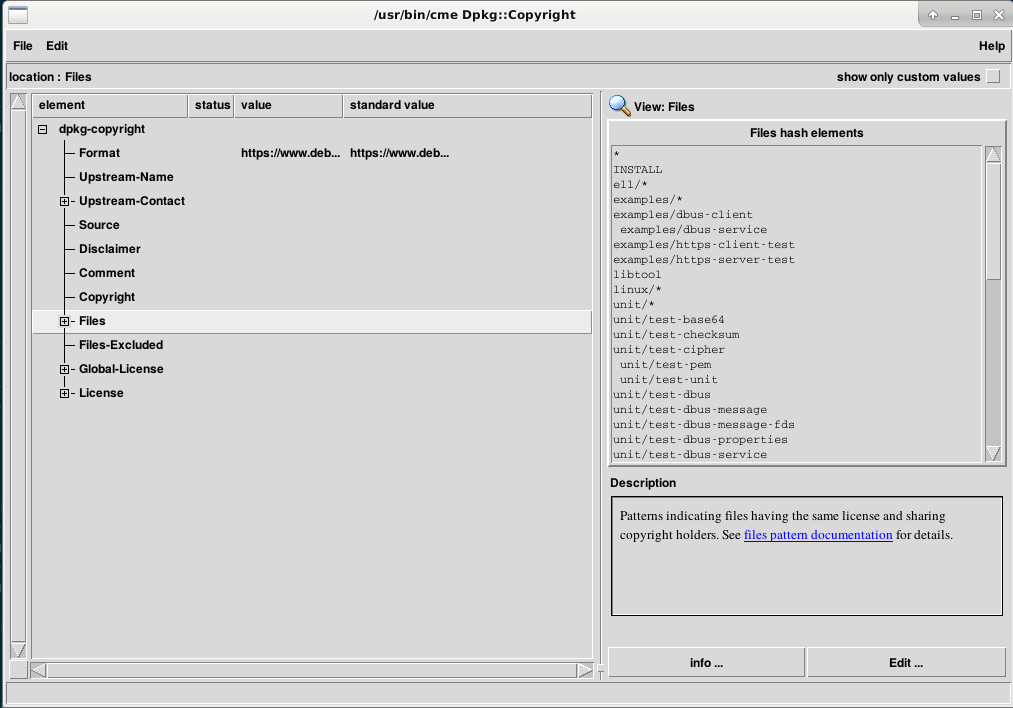
\includegraphics[width=0.7\hsize]{image201609/cme-gui.png}
\end{center}
\caption{cme GUI起動画面}
\label{fig:cme-gui}
 \end{minipage}
\end{figure}

これもlicensecheck2dep5と同様、完璧な出力はしてくれないため、出力
された debian/copyright ファイルを確認して修正する必要があります。
またUTF-8に対応しているため、ASCII文字以外でも正しく処理してくれます。

\subsubsection{debmake を使った debian/copyright の DEP5フォーマット化}

debmake コマンドの \texttt{-cc} オプションを使ってDEP5フォーマット化された
debian/copyright を作成することもできます。

\begin{commandline}
$ debmake -cc > debian/copyright
\end{commandline}

cme との違いは ファイルを列挙する点(cmeはワイルドカード($\ast$)でまとめる)
と 不要なファイル(例 debian/copyright)の内容まで確認してしまうなどがあります。
debmake は ソースパッケージ作成サポートツールなので、更新機能がまだないのだと
思います。個人的には今のところ debian ディレクトリ以下のファイルチェックにも
使える cme をお薦めします。

\subsubsection{license-reconcile による debian/copyright チェックサポート}


license-reconcile を使うことによって、
cme などで捕捉できないファイルのライセンスやコピーライトが debian/copyright が書かれているか、チェック
できるようにするツールとして\texttt{license-reconcile} があります。
これは\texttt{license-reconcile}パッケージによって提供されています。
例えば、今まで全てのファイルが\texttt{GPL-3+}でライセンスされていたプログラム
(図\ref{fig:example-copyright})に
\texttt{GPL-2+}でライセンスされている\texttt{hoge.png} ファイルが取り込まれた
とします。バイナリファイルなので cme などでは検知できません。

\begin{figure}[htbp]
\begin{center}
\begin{commandline}
Files: *
Copyright: 2016 foo bar <foo@example.org>
License: GPL-3+
\end{commandline}
\end{center}
\caption{debian/copyright 例}
\label{fig:example-copyright}
\end{figure}

debian/copyright に記載されているかチェックできるようにするため、
\texttt{debian/license-reconcile.yml} ファイルを用意し、図
\ref{fig:example-license-reconcile}のような内容を記述します。

\begin{figure}[htbp]
\begin{center}
\begin{commandline}
Rules:
 rules:
  -
   Glob: hoge.png
   License: GPL-2+
   Copyright: 2016 foo bar <foo@example.org>
\end{commandline}
\end{center}
\caption{debian/license-reconcile.yml 例}
\label{fig:example-license-reconcile}
\end{figure}

\texttt{license-reconcile}コマンド を実行すると以下のようなコピーライトミスマッチエラー
が出力されます(図\ref{fig:example-license-reconcile})。

\begin{figure}[htbp]
\begin{center}
\begin{commandline}
$ license-reconcile
License mismatch: File hoge.png has license GPL-2+ which does not match GPL-3+.\
at /usr/share/perl5/Debian/LicenseReconcile/App.pm line 222, <GEN0> line 3.
\end{commandline}
\end{center}
\caption{license-reconcile 実行例}
\label{fig:example-license-reconcile}
\end{figure}

debian/copyright に \texttt{hoge.png} に関するフィールド(図
\ref{fig:example-update-copyright})を追加し、再度
\texttt{license-reconcile} コマンドを実行するとラインセンスフィールドチェックエラーが
出力されなくなります。

\begin{figure}[htbp]
\begin{center}
\begin{commandline}
Files: hoge.png
Copyright: foo bar <foo@example.org>
License: GPL-2+
 This program is free software: you can redistribute it and/or modify
 it under the terms of the GNU General Public License as published by
 the Free Software Foundation, either version 2 of the License, or
 (at your option) any later version.
(省略)
\end{commandline}
\end{center}
\caption{debian/copyright 追記例}
\label{fig:example-update-copyright}
\end{figure}

\subsubsection{debian パッケージ側の対応}

上記では licensecheck や cme といった ツールを使うことによって debian/copyright ファイルを
DEP5 フォーマットに切り替えることができることを説明しましたが、debian/rules にチ
ェック用のターゲットを追加することのよって、パッケージのメンテナンス性が向上しま
す。図\ref{fig:example-update-rules} のように debian/rules へ追記し
\texttt{debian/rules update-debian-copyright}を実行することにより、DEP 5 フォー
マット の debian/copyright を debian/copyright.auto に出力します。

\begin{figure}[htbp]
\begin{center}
\begin{commandline}
# cme を使う場合
update-debian-copyright:
	cme update dpkg-copyright -file debian/copyright.auto
# licensecheck + licensecheck2dep5 を使う場合
update-debian-copyright:
        licensecheck --copyright -r `find * -type f` | \
                /usr/lib/cdbs/licensecheck2dep5 > debian/copyright.auto
\end{commandline}
\end{center}
\caption{debian/rules 追記例}
\label{fig:example-update-rules}
\end{figure}

\subsection{まとめ}

DEP5 フォーマットの簡単な内容紹介と、debian/copyright の DEP5 フォーマットするた
めのツールの使い方、debian パッケージでの利用方法について説明しました。
以下、まとめです。
\begin{itemize}
\item DEP 5 は Debian ポリシーの一部。しかしオプショナル扱い。
フォーマット詳細は
\url{https://www.debian.org/doc/packaging-manuals/copyright-format/1.0/}または
\url{/usr/share/doc/debian-policy/copyright-format-1.0.txt.gz}にある。

\item licensecheck ツールによって ソースからのライセンスとコピーライトホルダーを
抽出可能。そのままではDEP5フォーマットにならないため、licensecheck2dep5を使う。
\item cme と libconfig-model-dpkg-perl を使うことによって licensecheck +
licensecheck2dep5 同様のことが可能。岩松のお勧めはこちら。
\item license-reconcile を使うことによって cme などで補完できないファイルのチェ
ックができる。
\item 毎回 cme や licencecheck などのコマンドを実行するのではなく、debian/rules
に書いておくとメンテナンスが楽になる。
\end{itemize}

%201607 tokyo
%-------------------------------------------------------------------------------
%\dancersection{Debian Installer Screen対応 配布資料参照}{Roger}
%-------------------------------------------------------------------------------

%-------------------------------------------------------------------------------
\dancersection{Debian Trivia Quiz}{}
%-------------------------------------------------------------------------------

ところで、みなさん Debian 関連の話題においついていますか?Debian関連の話
題はメーリングリストをよんでいると追跡できます。ただよんでいるだけではは
りあいがないので、理解度のテストをします。特に一人だけでは意味がわからな
いところもあるかも知れません。みんなで一緒に読んでみましょう。

今回の出題範囲は\url{debian-devel-announce@lists.debian.org} や \url{debian-devel@lists.debian.org}に投稿された
内容とDebian Project Newsからです。

\small
\begin{multicols}{2}
%; whizzy-master ../debianmeetingresume201311.tex
% $B0J>e$N@_Dj$r$7$F$$$k$?$a!"$3$N%U%!%$%k$G(B M-x whizzytex $B$9$k$H!"(Bwhizzytex$B$,MxMQ$G$-$^$9!#(B
%

\santaku
{stable$BHG$N(Bjessie$B$G$bDs6!$,3+;O$5$l$?(Biceweasel$B$N%"%C%W%G!<%H!#%Q%C%1!<%8L>$,JQ$o$C$F$$$^$9!#2?$K$J$C$?$G$7$g$&$+(B}
{iceweasel-esr}
{firefox}
{firefox-esr}
{firefox-esr}
{$B%j!<%,%kLdBj$,$R$HCJMn$7!"(Bdebian$B$G$b(Bfirefox$B$H$7$FDs6!$G$-$k$3$H$K$J$j$^$7$?!#=>Mh$N(Bjessie$B$G$O(Biceweasel ver38esr$B$,Ds6!$5$l$F$$$^$7$?!#:#2s$O(Bfirefox-esr$B%Q%C%1!<%8$H$7$F(Bver45esr$B$NDs6!$,3+;O$5$l$^$7$?!#(B}

\santaku
{Debian Administrator$B!G(Bs Hanbook(Debian$B4IM}<T%O%s%I%V%C%/(B)$B$H$$$&%I%-%e%a%s%H$,$"$j$^$9!#KDBg$JNL$N%I%-%e%a%s%H$G$"$j$^$9$,!"$D$$$KF|K\8lHG$,%j%j!<%9$5$l$^$7$?!#K]Lu:n6H$KB?Bg$J9W8%$r$7$F$$$?$@$$$?J}$OC/$G$7$g$&$+!#(B}
{Ryuunosuke Ayanokouzi}
{Norimitsu Sugimoto}
{Hideki Yamane}
{Ryuunosuke Ayanokouzi}
{Debian$B4IM}<T%O%s%I%V%C%/$OL5NA$N(Bweb$BHG5Z$SEE;R=q@RHG!"M-NA$N=q@RHG$,$"$j$^$9!#:#8e$NK]Lu:n6H7QB3$N$?$a$K4sIU$rJg$C$F$$$^$9!#$J$*!"%j%j!<%9%"%J%&%s%9$N%Z!<%8$O<!$N(BURL$B$O<!$NDL$j$G$9!#(B\url{https://debian-handbook.info/2016/get-the-japanese-version-of-the-debian-administrators-handbook/}}

%; whizzy-master ../debianmeetingresume201311.tex
% $B0J>e$N@_Dj$r$7$F$$$k$?$a!"$3$N%U%!%$%k$G(B M-x whizzytex $B$9$k$H!"(Bwhizzytex$B$,MxMQ$G$-$^$9!#(B
%

\santaku
{quiz1}
{a}
{b}
{c}
{C}
{desc}

%; whizzy-master ../debianmeetingresume201311.tex
% $B0J>e$N@_Dj$r$7$F$$$k$?$a!"$3$N%U%!%$%k$G(B M-x whizzytex $B$9$k$H!"(Bwhizzytex$B$,MxMQ$G$-$^$9!#(B
%

\santaku
{unstable$B$K$F(BGCC$B$,(BTransition$B$5$l$^$7$?!#$5$F!"%P!<%8%g%s$O2?$K(BTransition$B$5$l$?$G$7$g$&$+(B}
{5.4}
{6.1}
{7.0}
{B}
{debian-devel-announce$B$K$F(BGCC-6$B$X(BTransition$B$5$l$^$7$?!#(BGCC-6$B$G$O(BC++14$B$,<BAu$5$l$F$$$^$9!#(BGNU Web$B%5%$%H$N!V(BPorting to GCC 6$B!W$N5-;v$r3NG'$7$F?7(BGCC$B$X0\9T$7$F$/$@$5$$!#%a!<%k!'!V(BTransition news: GCC 6 enabled by default$B!W(B\url{https://lists.debian.org/debian-devel-announce/2016/08/msg00001.html}}

\santaku
{unstalbe$B$K$F(Bperl$B$,(BTransition$B$5$l$^$7$?!#$5$F!"%P!<%8%g%s$O2?$K(BTransition$B$5$l$?$G$7$g$&$+(B}
{5.22}
{5.24}
{6.0}
{B}
{2016$BG/(B5$B7n$K%j%j!<%9$5$l$?(Bperl-5.24$B$X(BTransition$B$5$l$^$7$?!#(B2015$BG/%/%j%9%^%9$K$O(BPerl-6$B%j%j!<%9$NBg%K%e!<%9$,$"$j$^$7$?$,!"(BDebian$B$G:NMQ$5$l$k$K$O@h$,D9$=$&$G$9!#%a!<%k!'!V(Btransition: perl$B!W(B\url{https://bugs.debian.org/cgi-bin/bugreport.cgi?bug=830200}}

\santaku
{Linux Kernel$B$K$*$$$F<!$N(BLTS(=LongTermSupport)$B$H$9$k%P!<%8%g%s$N8uJd$,>e$,$C$F$-$^$7$?!#$5$F%P!<%8%g%s$O2?$G$7$g$&$+(B}
{4.8}
{4.9}
{4.10}
{B}
{stretch$B$N%j%j!<%97W2h$G$O(Blinux-4.10$B$r:NMQ$9$kM=Dj$H$7$?$?$a%U%j!<%:;~4|$rCY$i$;$k$3$H$K$7$F$$$^$7$?!#(BLTS$B$J%+!<%M%k$N%j%j!<%9$,Aa$$$+$i$H$$$C$F$9$G$K%"%J%&%s%9:Q$N%U%j!<%:;~4|$,Aa$^$k$3$H$O$J$$$H;W$$$^$9$,!"Cm;k$7$F$*$$$?$[$&$,$$$$$+$b$7$l$^$;$s!#%a!<%k!'!V(BLinux 4.9 will be next LTS$B!W(B\url{https://lists.debian.org/debian-release/2016/08/msg00147.html}}

%; whizzy-master ../debianmeetingresume201311.tex
% $B0J>e$N@_Dj$r$7$F$$$k$?$a!"$3$N%U%!%$%k$G(B M-x whizzytex $B$9$k$H!"(Bwhizzytex$B$,MxMQ$G$-$^$9!#(B
%

\santaku
{debain$B%Q%C%1!<%8$N%=!<%9%3!<%I$r%@%&%s%m!<%I$9$kJ}K!$O$"$k$+<ALd$,$"$j$^$7$?!#(BDD$B$NJ}$?$A$,0FFb$7$?%5!<%S%9$O$I$l$G$7$g$&$+!#(B}
{srcs.debian.org}
{srcs.debian.net}
{sources.debian.net}
{C}
{$B4Z9q$G>pJs9)3X$r3X$s$G$$$kBg3X1!@8$NJ}$+$i%;%-%e%j%F%#$N8&5f$N0l4D$GA4%=!<%9%3!<%I$,$[$7$$$H$N$3$H$G$7$?!#$=$N$[$+$K(Bdebmirror$B%3%^%s%I$r;H$&$H$h$$$H$$$&%"%I%P%$%9$b$"$j$^$7$?!#>pJs85(B:\url{https://lists.debian.org/debian-devel/2016/09/msg00118.html}}

%; whizzy-master ../debianmeetingresume201311.tex
% $B0J>e$N@_Dj$r$7$F$$$k$?$a!"$3$N%U%!%$%k$G(B M-x whizzytex $B$9$k$H!"(Bwhizzytex$B$,MxMQ$G$-$^$9!#(B
%

\santaku
{HP$B%(%s%?!<%W%i%$%:<R$+$i(BDebian Project$B$X%5!<%P$r4sIU$7$F$$$@$-$^$7$?!#$3$N%5!<%P$r;H$C$F(Bdebian.org$B$N%5!<%S%9$N:\$;BX$($,<B;\$5$l$^$9!#$5$F!"$I$NAH$_9g$o$;$,@5$7$$$G$7$g$&$+(B}
{ftp-master.debian.org$B$H(Bwww.debian.org}
{ftp-master.debian.org$B$H(Bsecurity.debian.org}
{www.debian.org$B$H(Bsecurity.debian.org}
{B}
{$B4sIU$$$?$@$$$?%5!<%P$O%+%J%@!"%"%a%j%+!"%*!<%9%H%i%j%"$K$"$k%5!<%P$N99?7$KMxMQ$9$kM=Dj$G$9!#6qBNE*$K$O(BDebian$B$N<gMW%5!<%S%9$G$"$k(Bftp-master.debian.org$B$H(Bsecurity.debian.org$B$K3d$jEv$F$7!"$=$NB>$N%3%"%5!<%S%9$N8~>e$K$bLrN)$F$kM=Dj$G$9!#(B\url{https://www.debian.org/News/2016/20161003}}

\end{multicols}
\normalsize

%for less page
%\printindex

\newpage

\begin{center}
本資料のライセンスについて
\end{center}

\begin{fontsize}{6}{6}

本資料はフリー・ソフトウェアです。あなたは、Free Software
Foundation が公表したGNU GENERAL PUBLIC LICENSEの "バージョン2"もしくはそれ以降
が定める条項に従って本プログラムを再頒布または変更することができ
ます。

本プログラムは有用とは思いますが、頒布にあたっては、市場性及び特
定目的適合性についての暗黙の保証を含めて、いかなる保証も行ないま
せん。詳細についてはGNU GENERAL PUBLIC LICENSE をお読みください。

\end{fontsize}

\begin{center}
ソースコードについて
\end{center}

本資料のソースコードは Git を使って\url{git://anonscm.debian.org/tokyodebian/monthly-report.git}
からダウンロードできます。以下に方法を示します。

\begin{commandline}
$ git clone git://anonscm.debian.org/tokyodebian/monthly-report.git
\end{commandline}
%$

\begin{multicols}{2}
 \begin{fontsize}{6}{6}
 \begin{verbatim}
            GNU GENERAL PUBLIC LICENSE
               Version 2, June 1991

 Copyright (C) 1989, 1991 Free Software Foundation, Inc.
    51 Franklin St, Fifth Floor, Boston, MA  02110-1301  USA
 Everyone is permitted to copy and distribute verbatim copies
 of this license document, but changing it is not allowed.

                Preamble

  The licenses for most software are designed to take away your
freedom to share and change it.  By contrast, the GNU General Public
License is intended to guarantee your freedom to share and change free
software--to make sure the software is free for all its users.  This
General Public License applies to most of the Free Software
Foundation's software and to any other program whose authors commit to
using it.  (Some other Free Software Foundation software is covered by
the GNU Library General Public License instead.)  You can apply it to
your programs, too.

  When we speak of free software, we are referring to freedom, not
price.  Our General Public Licenses are designed to make sure that you
have the freedom to distribute copies of free software (and charge for
this service if you wish), that you receive source code or can get it
if you want it, that you can change the software or use pieces of it
in new free programs; and that you know you can do these things.

  To protect your rights, we need to make restrictions that forbid
anyone to deny you these rights or to ask you to surrender the rights.
These restrictions translate to certain responsibilities for you if you
distribute copies of the software, or if you modify it.

  For example, if you distribute copies of such a program, whether
gratis or for a fee, you must give the recipients all the rights that
you have.  You must make sure that they, too, receive or can get the
source code.  And you must show them these terms so they know their
rights.

  We protect your rights with two steps: (1) copyright the software, and
(2) offer you this license which gives you legal permission to copy,
distribute and/or modify the software.

  Also, for each author's protection and ours, we want to make certain
that everyone understands that there is no warranty for this free
software.  If the software is modified by someone else and passed on, we
want its recipients to know that what they have is not the original, so
that any problems introduced by others will not reflect on the original
authors' reputations.

  Finally, any free program is threatened constantly by software
patents.  We wish to avoid the danger that redistributors of a free
program will individually obtain patent licenses, in effect making the
program proprietary.  To prevent this, we have made it clear that any
patent must be licensed for everyone's free use or not licensed at all.

  The precise terms and conditions for copying, distribution and
modification follow.

            GNU GENERAL PUBLIC LICENSE
   TERMS AND CONDITIONS FOR COPYING, DISTRIBUTION AND MODIFICATION

  0. This License applies to any program or other work which contains
a notice placed by the copyright holder saying it may be distributed
under the terms of this General Public License.  The "Program", below,
refers to any such program or work, and a "work based on the Program"
means either the Program or any derivative work under copyright law:
that is to say, a work containing the Program or a portion of it,
either verbatim or with modifications and/or translated into another
language.  (Hereinafter, translation is included without limitation in
the term "modification".)  Each licensee is addressed as "you".

Activities other than copying, distribution and modification are not
covered by this License; they are outside its scope.  The act of
running the Program is not restricted, and the output from the Program
is covered only if its contents constitute a work based on the
Program (independent of having been made by running the Program).
Whether that is true depends on what the Program does.

  1. You may copy and distribute verbatim copies of the Program's
source code as you receive it, in any medium, provided that you
conspicuously and appropriately publish on each copy an appropriate
copyright notice and disclaimer of warranty; keep intact all the
notices that refer to this License and to the absence of any warranty;
and give any other recipients of the Program a copy of this License
along with the Program.

You may charge a fee for the physical act of transferring a copy, and
you may at your option offer warranty protection in exchange for a fee.

  2. You may modify your copy or copies of the Program or any portion
of it, thus forming a work based on the Program, and copy and
distribute such modifications or work under the terms of Section 1
above, provided that you also meet all of these conditions:

    a) You must cause the modified files to carry prominent notices
    stating that you changed the files and the date of any change.

    b) You must cause any work that you distribute or publish, that in
    whole or in part contains or is derived from the Program or any
    part thereof, to be licensed as a whole at no charge to all third
    parties under the terms of this License.

    c) If the modified program normally reads commands interactively
    when run, you must cause it, when started running for such
    interactive use in the most ordinary way, to print or display an
    announcement including an appropriate copyright notice and a
    notice that there is no warranty (or else, saying that you provide
    a warranty) and that users may redistribute the program under
    these conditions, and telling the user how to view a copy of this
    License.  (Exception: if the Program itself is interactive but
    does not normally print such an announcement, your work based on
    the Program is not required to print an announcement.)

These requirements apply to the modified work as a whole.  If
identifiable sections of that work are not derived from the Program,
and can be reasonably considered independent and separate works in
themselves, then this License, and its terms, do not apply to those
sections when you distribute them as separate works.  But when you
distribute the same sections as part of a whole which is a work based
on the Program, the distribution of the whole must be on the terms of
this License, whose permissions for other licensees extend to the
entire whole, and thus to each and every part regardless of who wrote it.

Thus, it is not the intent of this section to claim rights or contest
your rights to work written entirely by you; rather, the intent is to
exercise the right to control the distribution of derivative or
collective works based on the Program.

In addition, mere aggregation of another work not based on the Program
with the Program (or with a work based on the Program) on a volume of
a storage or distribution medium does not bring the other work under
the scope of this License.

  3. You may copy and distribute the Program (or a work based on it,
under Section 2) in object code or executable form under the terms of
Sections 1 and 2 above provided that you also do one of the following:

    a) Accompany it with the complete corresponding machine-readable
    source code, which must be distributed under the terms of Sections
    1 and 2 above on a medium customarily used for software interchange; or,

    b) Accompany it with a written offer, valid for at least three
    years, to give any third party, for a charge no more than your
    cost of physically performing source distribution, a complete
    machine-readable copy of the corresponding source code, to be
    distributed under the terms of Sections 1 and 2 above on a medium
    customarily used for software interchange; or,

    c) Accompany it with the information you received as to the offer
    to distribute corresponding source code.  (This alternative is
    allowed only for noncommercial distribution and only if you
    received the program in object code or executable form with such
    an offer, in accord with Subsection b above.)

The source code for a work means the preferred form of the work for
making modifications to it.  For an executable work, complete source
code means all the source code for all modules it contains, plus any
associated interface definition files, plus the scripts used to
control compilation and installation of the executable.  However, as a
special exception, the source code distributed need not include
anything that is normally distributed (in either source or binary
form) with the major components (compiler, kernel, and so on) of the
operating system on which the executable runs, unless that component
itself accompanies the executable.

If distribution of executable or object code is made by offering
access to copy from a designated place, then offering equivalent
access to copy the source code from the same place counts as
distribution of the source code, even though third parties are not
compelled to copy the source along with the object code.

  4. You may not copy, modify, sublicense, or distribute the Program
except as expressly provided under this License.  Any attempt
otherwise to copy, modify, sublicense or distribute the Program is
void, and will automatically terminate your rights under this License.
However, parties who have received copies, or rights, from you under
this License will not have their licenses terminated so long as such
parties remain in full compliance.

  5. You are not required to accept this License, since you have not
signed it.  However, nothing else grants you permission to modify or
distribute the Program or its derivative works.  These actions are
prohibited by law if you do not accept this License.  Therefore, by
modifying or distributing the Program (or any work based on the
Program), you indicate your acceptance of this License to do so, and
all its terms and conditions for copying, distributing or modifying
the Program or works based on it.

  6. Each time you redistribute the Program (or any work based on the
Program), the recipient automatically receives a license from the
original licensor to copy, distribute or modify the Program subject to
these terms and conditions.  You may not impose any further
restrictions on the recipients' exercise of the rights granted herein.
You are not responsible for enforcing compliance by third parties to
this License.

  7. If, as a consequence of a court judgment or allegation of patent
infringement or for any other reason (not limited to patent issues),
conditions are imposed on you (whether by court order, agreement or
otherwise) that contradict the conditions of this License, they do not
excuse you from the conditions of this License.  If you cannot
distribute so as to satisfy simultaneously your obligations under this
License and any other pertinent obligations, then as a consequence you
may not distribute the Program at all.  For example, if a patent
license would not permit royalty-free redistribution of the Program by
all those who receive copies directly or indirectly through you, then
the only way you could satisfy both it and this License would be to
refrain entirely from distribution of the Program.

If any portion of this section is held invalid or unenforceable under
any particular circumstance, the balance of the section is intended to
apply and the section as a whole is intended to apply in other
circumstances.

It is not the purpose of this section to induce you to infringe any
patents or other property right claims or to contest validity of any
such claims; this section has the sole purpose of protecting the
integrity of the free software distribution system, which is
implemented by public license practices.  Many people have made
generous contributions to the wide range of software distributed
through that system in reliance on consistent application of that
system; it is up to the author/donor to decide if he or she is willing
to distribute software through any other system and a licensee cannot
impose that choice.

This section is intended to make thoroughly clear what is believed to
be a consequence of the rest of this License.

  8. If the distribution and/or use of the Program is restricted in
certain countries either by patents or by copyrighted interfaces, the
original copyright holder who places the Program under this License
may add an explicit geographical distribution limitation excluding
those countries, so that distribution is permitted only in or among
countries not thus excluded.  In such case, this License incorporates
the limitation as if written in the body of this License.

  9. The Free Software Foundation may publish revised and/or new versions
of the General Public License from time to time.  Such new versions will
be similar in spirit to the present version, but may differ in detail to
address new problems or concerns.

Each version is given a distinguishing version number.  If the Program
specifies a version number of this License which applies to it and "any
later version", you have the option of following the terms and conditions
either of that version or of any later version published by the Free
Software Foundation.  If the Program does not specify a version number of
this License, you may choose any version ever published by the Free Software
Foundation.

  10. If you wish to incorporate parts of the Program into other free
programs whose distribution conditions are different, write to the author
to ask for permission.  For software which is copyrighted by the Free
Software Foundation, write to the Free Software Foundation; we sometimes
make exceptions for this.  Our decision will be guided by the two goals
of preserving the free status of all derivatives of our free software and
of promoting the sharing and reuse of software generally.

                NO WARRANTY

  11. BECAUSE THE PROGRAM IS LICENSED FREE OF CHARGE, THERE IS NO WARRANTY
FOR THE PROGRAM, TO THE EXTENT PERMITTED BY APPLICABLE LAW.  EXCEPT WHEN
OTHERWISE STATED IN WRITING THE COPYRIGHT HOLDERS AND/OR OTHER PARTIES
PROVIDE THE PROGRAM "AS IS" WITHOUT WARRANTY OF ANY KIND, EITHER EXPRESSED
OR IMPLIED, INCLUDING, BUT NOT LIMITED TO, THE IMPLIED WARRANTIES OF
MERCHANTABILITY AND FITNESS FOR A PARTICULAR PURPOSE.  THE ENTIRE RISK AS
TO THE QUALITY AND PERFORMANCE OF THE PROGRAM IS WITH YOU.  SHOULD THE
PROGRAM PROVE DEFECTIVE, YOU ASSUME THE COST OF ALL NECESSARY SERVICING,
REPAIR OR CORRECTION.

  12. IN NO EVENT UNLESS REQUIRED BY APPLICABLE LAW OR AGREED TO IN WRITING
WILL ANY COPYRIGHT HOLDER, OR ANY OTHER PARTY WHO MAY MODIFY AND/OR
REDISTRIBUTE THE PROGRAM AS PERMITTED ABOVE, BE LIABLE TO YOU FOR DAMAGES,
INCLUDING ANY GENERAL, SPECIAL, INCIDENTAL OR CONSEQUENTIAL DAMAGES ARISING
OUT OF THE USE OR INABILITY TO USE THE PROGRAM (INCLUDING BUT NOT LIMITED
TO LOSS OF DATA OR DATA BEING RENDERED INACCURATE OR LOSSES SUSTAINED BY
YOU OR THIRD PARTIES OR A FAILURE OF THE PROGRAM TO OPERATE WITH ANY OTHER
PROGRAMS), EVEN IF SUCH HOLDER OR OTHER PARTY HAS BEEN ADVISED OF THE
POSSIBILITY OF SUCH DAMAGES.

             END OF TERMS AND CONDITIONS

        How to Apply These Terms to Your New Programs

  If you develop a new program, and you want it to be of the greatest
possible use to the public, the best way to achieve this is to make it
free software which everyone can redistribute and change under these terms.

  To do so, attach the following notices to the program.  It is safest
to attach them to the start of each source file to most effectively
convey the exclusion of warranty; and each file should have at least
the "copyright" line and a pointer to where the full notice is found.

    <one line to give the program's name and a brief idea of what it does.>
    Copyright (C) <year>  <name of author>

    This program is free software; you can redistribute it and/or modify
    it under the terms of the GNU General Public License as published by
    the Free Software Foundation; either version 2 of the License, or
    (at your option) any later version.

    This program is distributed in the hope that it will be useful,
    but WITHOUT ANY WARRANTY; without even the implied warranty of
    MERCHANTABILITY or FITNESS FOR A PARTICULAR PURPOSE.  See the
    GNU General Public License for more details.

    You should have received a copy of the GNU General Public License
    along with this program; if not, write to the Free Software
    Foundation, Inc., 51 Franklin St, Fifth Floor, Boston, MA  02110-1301 USA


Also add information on how to contact you by electronic and paper mail.

If the program is interactive, make it output a short notice like this
when it starts in an interactive mode:

    Gnomovision version 69, Copyright (C) year  name of author
    Gnomovision comes with ABSOLUTELY NO WARRANTY; for details type `show w'.
    This is free software, and you are welcome to redistribute it
    under certain conditions; type `show c' for details.

The hypothetical commands `show w' and `show c' should show the appropriate
parts of the General Public License.  Of course, the commands you use may
be called something other than `show w' and `show c'; they could even be
mouse-clicks or menu items--whatever suits your program.

You should also get your employer (if you work as a programmer) or your
school, if any, to sign a "copyright disclaimer" for the program, if
necessary.  Here is a sample; alter the names:

  Yoyodyne, Inc., hereby disclaims all copyright interest in the program
  `Gnomovision' (which makes passes at compilers) written by James Hacker.

  <signature of Ty Coon>, 1 April 1989
  Ty Coon, President of Vice

This General Public License does not permit incorporating your program into
proprietary programs.  If your program is a subroutine library, you may
consider it more useful to permit linking proprietary applications with the
library.  If this is what you want to do, use the GNU Library General
Public License instead of this License.
 \end{verbatim}
 \end{fontsize}
\end{multicols}

\begin{center}
Debian オープンユーズロゴ ライセンス
\end{center}

\begin{multicols}{2}
 \begin{fontsize}{6}{6}
 \begin{verbatim}

Copyright (c) 1999 Software in the Public Interest
Permission is hereby granted, free of charge, to any person
obtaining a copy of this software and associated documentation
files (the "Software"), to deal in the Software without restriction,
including without limitation the rights to use, copy, modify, merge,
publish, distribute, sublicense, and/or sell copies of the Software,
and to permit persons to whom the Software is furnished to do so,
subject to the following conditions:

The above copyright notice and this permission notice shall be
included in all copies or substantial portions of the Software.

THE SOFTWARE IS PROVIDED "AS IS", WITHOUT WARRANTY OF ANY
KIND, EXPRESS OR IMPLIED, INCLUDING BUT NOT LIMITED TO THE
WARRANTIES OF MERCHANTABILITY, FITNESS FOR A PARTICULAR PURPOSE AND
NONINFRINGEMENT. IN NO EVENT SHALL THE AUTHORS OR COPYRIGHT HOLDERS
BE LIABLE FOR ANY CLAIM, DAMAGES OR OTHER LIABILITY, WHETHER IN
AN ACTION OF CONTRACT, TORT OR OTHERWISE, ARISING FROM, OUT OF OR
IN CONNECTION WITH THE SOFTWARE OR THE USE OR OTHER DEALINGS IN
THE SOFTWARE.
 \end{verbatim}
 \end{fontsize}
\end{multicols}

% 問題と回答が同じみひらきにならないようにする
%\cleartoevenpage
%-------------------------------------------------------------------------------
\dancersection{Debian Trivia Quiz 問題回答}{}
%-------------------------------------------------------------------------------

 Debian Trivia Quiz の問題回答です。
 あなたは何問わかりましたか? \\
 %回答はdebianmeetingresume2014-fuyu.jqzというファイルに生成されるので、
 %それを手動でコピペして使う。
 % ここからコピペ
 % FIXME 問題が全部はいったらコピペすること
 %(progn (next-line 1)(insert-file "debianmeetingresume2013-fuyu.jqz") )
 \begin{enumerate}
 \item C リーガル問題がひと段落し、debianでもfirefoxとして提供できることになりました。従来のjessieではiceweasel ver38esrが提供されていました。今回はfirefox-esrパッケージとしてver45esrの提供が開始されました。\\
 \item A Debian管理者ハンドブックは無料のweb版及び電子書籍版、有料の書籍版があります。今後の翻訳作業継続のために寄付を募っています。なお、リリースアナウンスのページは次のURLは次の通りです。\url {https://debian-handbook.info/2016/get-the-japanese-version-of-the-debian-administrators-handbook/}\\
\item  B \url {https://debconf16.debconf.org/}の案内にあるとおり、南アフリカのケープタウンで行われました。日本から参加した人がいますので、後でどんな感じだったか聞いてみましょう。例年通りであれば、セッションのビデオが後日公開されると思います。\\
\item  A Transition freezeが2016-11-05、Mandatory 10-day migrationsが2016-12-05、Soft freezeが2017-01-05、Full freezeが2017-02-05の予定となっています。新しいパッケージをStretchに含めたい場合はお早めに。\\
\item  B debian-devel-announceにてGCC-6へTransitionされました。GCC-6ではC++14が実装されています。GNU Webサイトの「Porting to GCC 6」の記事を確認して新GCCへ移行してください。メール:「Transition news: GCC 6 enabled by default」\url {https://lists.debian.org/debian-devel-announce/2016/08/msg00001.html}\\
\item  B 2016年5月にリリースされたperl-5.24へTransitionされました。2015年クリスマスにはPerl-6リリースの大ニュースがありましたが、Debianで採用されるには先が長そうです。メール:「transition: perl」\url {https://bugs.debian.org/cgi-bin/bugreport.cgi?bug=830200}\\
\item  B stretchのリリース計画ではlinux-4.10を採用する予定としたためフリーズ時期を遅らせることにしていました。LTSなカーネルのリリースが早いからといってすでにアナウンス済のフリーズ時期が早まることはないと思いますが、注視しておいたほうがいいかもしれません。メール:「Linux 4.9 will be next LTS」\url {https://lists.debian.org/debian-release/2016/08/msg00147.html}\\
\item  C 韓国で情報工学を学んでいる大学院生の方からセキュリティの研究の一環で全ソースコードがほしいとのことでした。そのほかにdebmirrorコマンドを使うとよいというアドバイスもありました。情報元:\url {https://lists.debian.org/debian-devel/2016/09/msg00118.html}\\
\item  B 寄付いただいたサーバはカナダ、アメリカ、オーストラリアにあるサーバの更新に利用する予定です。具体的にはDebianの主要サービスであるftp-master.debian.orgとsecurity.debian.orgに割り当てし、その他のコアサービスの向上にも役立てる予定です。\url {https://www.debian.org/News/2016/20161003}\\

\end{enumerate}

% add page to even number
%\newpage
%\cleartoevenpage

\newpage
\thispagestyle{empty}\mbox{}
\newpage

\thispagestyle{empty}
{
\large
\begin{itembox}{\bf 『あんどきゅめんてっど でびあん』について}
本書は、東京および関西周辺で毎月行なわれている『東京エリア Debian 勉強会』および
『関西 Debian 勉強会』で
使用された資料・小ネタ・必殺技などを一冊にまとめたものです。
% FIXME: 範囲を修正すること。
収録範囲は2016/06〜2016/11まで+2016/04関西の収録漏れ分。
内容は無保証、つっこみなどがあれば勉強会にて。
\end{itembox}
}

\vspace*{13cm}
{\color{dancerlightblue}\rule{\hsize}{1mm}}
\vspace{2mm}

\includegraphics[width=2cm]{image200502/openlogo-nd.eps}
\noindent \Large \bf あんどきゅめんてっど でびあん 2016年冬号\\
\noindent \normalfont 2016年12月29日 \hspace{5mm}  初版第1刷発行\\
\noindent \normalfont 東京エリア Debian 勉強会/関西Debian 勉強会 (編集・印刷・発行)\\
{\color{dancerdarkblue}\rule{\hsize}{1mm}}

\end{document}
